\documentclass[14pt]{extarticle}

\usepackage[table]{xcolor} % colored lines for tables
%\usepackage[normalem]{ulem} % strike through text
\usepackage{amsmath,mathtools,amsfonts,amsthm,amssymb,hyperref}
\usepackage{parskip,geometry,latexsym,bookmark,mathtools,float,cancel}
\usepackage{tcolorbox,bm,minted}

\newtheorem{defn}{Definition}
\newtheorem{thm}{Theorem}
\newtheorem{claim}{Claim}
\newtheorem{lemma}{Lemma}

\newcommand{\dps}{\displaystyle}
\newcommand{\es}{\varnothing}
\newcommand{\fbl}{\underline{\hspace{1cm}}\,\,}
\newcommand{\R}{\mathbb{R}}
\newcommand{\Q}{\mathbb{Q}}
\newcommand{\Z}{\mathbb{Z}}
\newcommand{\from}{\leftarrow}
\newcommand{\true}{{\bf t}}
\newcommand{\false}{{\bf c}}
\newcommand{\bic}{\leftrightarrow}
\newcommand{\da}{\downarrow}
\newcommand{\cyda}{{\cy \(\downarrow\)}}
\newcommand{\fa}{\forall}
\newcommand{\te}{\exists}
\newcommand{\cy}{\color{cyan}}

\newcommand{\colsq}[1]{{\color{#1} $\blacksquare$}}

\newcommand{\base}[1]{{\cy #1}} % for log bases
\newcommand{\floor}[1]{{\left\lfloor#1\right\rfloor}}
\newcommand{\ceil}[1]{{\left\lceil#1\right\rceil}}
\newcommand\Ccancel[2][black]{\renewcommand\CancelColor{\color{#1}}\cancel{#2}}
\newcommand\Cbcancel[2][black]{\renewcommand\CancelColor{\color{#1}}\bcancel{#2}}

\renewcommand{\arraystretch}{1.2}

\hypersetup{colorlinks,allcolors=blue,linktoc=all}
\geometry{a4paper}
\geometry{margin=0.42in}

\title{Solutions to Chapter 9, Susanna Epp Discrete Math 5th Edition}

\author{https://github.com/spamegg1}

\begin{document}
\maketitle
\tableofcontents

\section{Exercise Set 9.1}

\subsection{Exercise 1}
Toss two coins 30 times and make a table showing the relative frequencies of 0, 1, and 2 heads. How do your 
values compare with those shown in Table 9.1.1?

\begin{proof}
\begin{center}
\arrayrulecolor{cyan}
\begin{tabular}{|c|c|c|}
\hline
{\bf\cy Event} & {\bf\cy Freq.} & {\bf\cy Rel. freq.} \\
\hline
2 heads obtained & 7 & 23.33\% \\
\hline
1 head obtained & 16 & 53.33\% \\
\hline
0 heads obtained & 7 & 23.33\% \\
\hline
\end{tabular}
\arrayrulecolor{black} % change it back!
\end{center}
\end{proof}

\subsection{Exercise 2}
In the example of tossing two quarters, what is the probability that at least one head is obtained? that coin 
$A$ is a head? that coins $A$ and $B$ are either both
heads or both tails?

\begin{proof}
3/4, 1/2, 1/2
\end{proof}

{\bf \cy In $3-6$ use the sample space given in example 9.1.1. Write each event as a set and compute its 
probability.}

\subsection{Exercise 3}
The event that the chosen card is red and is not a face card.

\begin{proof}
\(\{1\diamondsuit, 2\diamondsuit, 3\diamondsuit, 4\diamondsuit, 5\diamondsuit, 6\diamondsuit, 7\diamondsuit, 
8\diamondsuit, 9\diamondsuit, 10\diamondsuit, 1\heartsuit, 2\heartsuit, 3\heartsuit, 4\heartsuit, 5\heartsuit\), 

\(6\heartsuit, 7\heartsuit, 8\heartsuit, 9\heartsuit, 10\heartsuit\}\), probability \(= 20/52 \approx 38.5\%\)
\end{proof}

\subsection{Exercise 4}
The event that the chosen card is black and has an even number on it.

\begin{proof}
\(\{2\spadesuit, 4\spadesuit, 6\spadesuit, 8\spadesuit, 10\spadesuit, 2\clubsuit, 4\clubsuit, 6\clubsuit, 
8\clubsuit, 10\clubsuit\}\), probability \(= 10/52 \approx 19.2\%\)
\end{proof}

\subsection{Exercise 5}
The event that the denomination of the chosen card is at least 10 (counting aces high).

\begin{proof}
\(\{10\spadesuit, J\spadesuit, Q\spadesuit, K\spadesuit, A\spadesuit, 10\diamondsuit, J\diamondsuit, Q\diamondsuit, 
K\diamondsuit, A\diamondsuit, 10\heartsuit, J\heartsuit, Q\heartsuit, K\heartsuit, A\heartsuit\), 

\(10\clubsuit, J\clubsuit, Q\clubsuit, K\clubsuit, A\clubsuit\}\), probability \(= 20/52=5/13 \approx 38.5\%\)
\end{proof}

\subsection{Exercise 6}
The event that the denomination of the chosen card is at most 4 (counting aces high).

\begin{proof}
\(\{2\clubsuit, 2\heartsuit, 2\spadesuit, 2\diamondsuit, 3\clubsuit, 3\heartsuit, 3\spadesuit, 3\diamondsuit, 
4\clubsuit, 4\heartsuit, 4\spadesuit, 4\diamondsuit\}\), probability \(= 12/52 \approx 23.0\%\)
\end{proof}

{\bf \cy In $7-10$, use the sample space given in example 9.1.2. Write each of the following events as a set and 
compute its probability.}

\subsection{Exercise 7}
The event that the sum of the numbers showing face up is 8.

\begin{proof}
\(\{26, 35, 44, 53, 62\}\), probability \(= 5/36 \approx 13.9\%\)
\end{proof}

\subsection{Exercise 8}
The event that the numbers showing face up are the same.

\begin{proof}
\(\{11, 22, 33, 44, 55, 66\}\), probability \(= 6/36 \approx 16.6\%\)
\end{proof}

\subsection{Exercise 9}
The event that the sum of the numbers showing face up is at most 6.

\begin{proof}
\(\{11, 12, 13, 14, 15, 21, 22, 23, 24, 31, 32, 33, 41, 42, 51\}\), prob. \(= 15/36 \approx 41.6\%\)
\end{proof}

\subsection{Exercise 10}
The event that the sum of the numbers showing face up is at least 9.

\begin{proof}
\(\{36, 45, 46, 54, 55, 56, 63, 64, 65, 66\}\), probability \(= 10/36 \approx 27.7\%\)
\end{proof}

\subsection{Exercise 11}
Suppose that a coin is tossed three times and the side showing face up on each toss is noted. Suppose also that on 
each toss heads and tails are equally likely. Let \(HHT\) indicate the outcome heads on the first two tosses and 
tails on the third, \(THT\) the outcome tails on the first and third tosses and heads on the second, and so forth.

\subsubsection{(a)}
List the eight elements in the sample space whose outcomes are all the possible head-tail sequences obtained in the 
three tosses.

\begin{proof}
\(\{HHH, HHT, HTH, HTT, THH, THT, TTH, TTT\}\)
\end{proof}

\subsubsection{(b)}
Write each of the following events as a set and find its probability:

(i) The event that exactly one toss results in a head.

(ii) The event that at least two tosses result in a head.

(iii) The event that no head is obtained.

\begin{proof}
(i) \(\{HTT, THT, TTH\}\), probability \(= 3/8 = 37.5\%\)

(ii) \(\{HHT, HTH, THH, HHH\}\), probability \(= 4/8 = 50.0\%\)

(iii) \(\{TTT\}\), probability \(= 1/8 = 12.5\%\)
\end{proof}

\subsection{Exercise 12}
Suppose that each child born is equally likely to be a boy or a girl. Consider a family with exactly three children. 
Let \(BBG\) indicate that the first two children born are boys and the third child is a girl, let \(GBG\) indicate 
that the first and third children born are girls and the second is a boy, and so forth.

\subsubsection{(a)}
List the eight elements in the sample space whose outcomes are all possible genders of the three children.

\begin{proof}
\(\{BBB, BBG, BGB, BGG, GBB, GBG, GGB, GGG\}\)
\end{proof}

\subsubsection{(b)}
Write each of the events in the next column as a set and find its probability.

(i) The event that exactly one child is a girl.

(ii) The event that at least two children are girls.

(iii) The event that no child is a girl.

\begin{proof}
(i) \(\{GBB, BGB, BBG\}\), probability \(= 3/8 = 37.5\%\)

(ii) \(\{GGB, GBG, BGG, GGG\}\), probability \(= 4/8 = 50\%\)

(iii) \(\{BBB\}\), probability \(= 1/8 = 12.5\%\)
\end{proof}

\subsection{Exercise 13}
Suppose that on a true/false exam you have no idea at all about the answers to three questions. You choose answers 
randomly and therefore have a 50–50 chance of being correct on any one question. Let \(CCW\) indicate that you were 
correct on the first two questions and wrong on the third, let \(WCW\) indicate that you were wrong on the first and 
third questions and correct on the second, and so forth.

\subsubsection{(a)}
List the elements in the sample space whose outcomes are all possible sequences of correct and incorrect responses 
on your part.

\begin{proof}
\(\{CCC, CCW, CWC, CWW, WCC, WCW, WWC, WWW\}\)
\end{proof}

\subsubsection{(b)}
Write each of the following events as a set and find its probability:

(i) The event that exactly one answer is correct.

(ii) The event that at least two answers are correct.

(iii) The event that no answer is correct.

\begin{proof}
(i) \(\{CWW, WCW, WWC\}\), probability \(= 3/8 = 37.5\%\)

(ii) \(\{CCW, CWC, WCC, CCC\}\), probability \(= 4/8 = 50\%\)

(iii) \(\{WWW\}\), probability \(= 1/8 = 12.5\%\)
\end{proof}

\subsection{Exercise 14}
Three people have been exposed to a certain illness. Once exposed, a person has a 50-50 chance of actually becoming ill.

\subsubsection{(a)}
What is the probability that exactly one of the people becomes ill?

\begin{proof}
probability \(= 3/8 = 37.5\%\)
\end{proof}

\subsubsection{(b)}
What is the probability that at least two of the people become ill?

\begin{proof}
probability \(= 4/8 = 50\%\)
\end{proof}

\subsubsection{(c)}
What is the probability that none of the three people becomes ill?

\begin{proof}
probability \(= 1/8 = 12.5\%\)
\end{proof}

\subsection{Exercise 15}
When discussing counting and probability, we often consider situations that may appear frivolous or of little practical 
value, such as tossing coins, choosing cards, or rolling dice. The reason is that these relatively simple examples 
serve as models for a wide variety of more complex situations in the real world. In light of this remark, 
comment on the relationship between your answer to exercise 11 and your answers to exercises $12-14$.

\begin{proof}
The answers to exercises 11, 12, 13, 14 are the same, because all 4 situations are modeled exactly the same way.
They each consist of 3 instances of the same event, each of which has 2 possible outcomes with 50\% probability (heads 
or tails, boy or girl, correct or incorrect, ill or not ill). They each have a sample space with 8 elements 
following the same pattern.
\end{proof}

\subsection{Exercise 16}
Two faces of a six-sided die are painted red, two are painted blue, and two are painted yellow. The die is rolled 
three times, and the colors that appear face up on the first, second, and third rolls are recorded.


\subsubsection{(a)}
Let \(BBR\) denote the outcome where the color appearing face up on the first and second rolls is blue and the color 
appearing face up on the third roll is red. Because there are as many faces of one color as of any other, the 
outcomes of this experiment are equally likely. List all 27 possible outcomes.

\begin{proof}
\(\{RRR, RRB, RRY, RBR, RBB, RBY, RYR, RYB, RYY,\) 

\(BRR, BRB, BRY, BBR, BBB, BBY, BYR, BYB, BYY,\)

\(YRR, YRB, YRY, YBR, YBB, YBY, YYR, YYB, YYY\}\)
\end{proof}

\subsubsection{(b)}
Consider the event that all three rolls produce different colors. One outcome in this event is \(RBY\) and another 
\(RYB\). List all outcomes in the event. What is the probability of the event?

\begin{proof}
\(\{RBY, RYB, YBR, BRY, BYR, YRB\}\), probability \(= 6/27 = 2/9 \approx 22.2\%\)
\end{proof}

\subsubsection{(c)}
Consider the event that two of the colors that appear face up are the same. One outcome in this event is \(RRB\) and 
another is \(RBR\). List all outcomes in the event. What is the probability of the event?

\begin{proof}
\(\{RRB, RBR, BRR, RRY, RYR, YRR, BBR, BRB, RBB, BBY, BYB, YBB,\)

\(YYR, YRY, RYY, YYB, YBY, BYY\}\), probability \(= 18/27 = 2/3 \approx 66.6\%\)
\end{proof}

\subsection{Exercise 17}
Consider the situation described in exercise 16.

\subsubsection{(a)}
Find the probability of the event that exactly one of the colors that appears face up is red.

\begin{proof}
\(\{RBB, RBY, RYB, RYY, BRB, BRY, BBR, BYR, YRB, YRY, YBR, YYR\}\), 

probability \(= 12/27 = 4/9 \approx 44.4\%\)
\end{proof}

\subsubsection{(b)}
Find the probability of the event that at least one of the colors that appears face up is red.

\begin{proof}
\(\{RRR, RRB, RRY, RBR, RBB, RBY, RYR, RYB, RYY, BRR, BRB, BRY,\) 

\(BBR, BYR, YRR, YRB, YRY, YBR, YYR\}\), probability \(= 20/27 \approx 74\%\)
\end{proof}

\subsection{Exercise 18}
An urn contains two blue balls (denoted \(B_1\) and \(B_2\)) and one white ball (denoted \(W\)). One ball is 
drawn, its color is recorded, and it is replaced in the urn. Then another ball is drawn, and its color is recorded.

\subsubsection{(a)}
Let \(B_1 W\) denote the outcome that the first ball drawn is \(B_1\) and the second ball drawn is \(W\). Because the 
first ball is replaced before the second ball is drawn, the outcomes of the experiment are equally likely. List all 
nine possible outcomes of the experiment.

\begin{proof}
\(\{B_1B_1, B_1B_2, B_1W, B_2B_1, B_2B_2, B_2W, WB_1, WB_2, WW\}\)
\end{proof}

\subsubsection{(b)}
Consider the event that the two balls that are drawn are both blue. List all outcomes in the event. 
What is the probability of the event?

\begin{proof}
\(\{B_1B_1, B_1B_2, B_2B_1, B_2B_2\}\), probability \(= 4/9 \approx 44.4\%\)
\end{proof}

\subsubsection{(c)}
Consider the event that the two balls that are drawn are of different colors. List all outcomes in the event. 
What is the probability of the event?

\begin{proof}
\(\{B_1W, B_2W, WB_1, WB_2\}\), probability \(= 4/9 \approx 44.4\%\)
\end{proof}

\subsection{Exercise 19}
An urn contains two blue balls (denoted \(B_1\) and \(B_2\)) and three white balls (denoted \(W_1, W_2\), and 
\(W_3\)). One ball is drawn, its color is recorded, and it is replaced in the urn. Then another ball is drawn and its 
color is recorded.

\subsubsection{(a)}
Let \(B_1 W_2\) denote the outcome that the first ball drawn is \(B_1\) and the second ball drawn is \(W_2\). 
Because the first ball is replaced before the second ball is drawn, the outcomes of the experiment are equally 
likely. List all 25 possible outcomes of the experiment.

\begin{proof}
\(\{B_1B_1, B_1B_2, B_1W_1, B_1W_2, B_1W_3\), 

\(B_2B_1, B_2B_2, B_2W_1, B_2W_2, B_2W_3\), 

\(W_1B_1, W_1B_2, W_1W_1, W_1W_2, W_1W_3\), 

\(W_2B_1, W_2B_2, W_2W_1, W_2W_2, W_2W_3\), 

\(W_3B_1, W_3B_2, W_3W_1, W_3W_2, W_3W_3\}\)
\end{proof}

\subsubsection{(b)}
Consider the event that the first ball that is drawn is blue. List all outcomes in the event. 
What is the probability of the event?

\begin{proof}
\(\{B_1B_1, B_1B_2, B_1W_1, B_1W_2, B_1W_3, B_2B_1, B_2B_2, B_2W_1, B_2W_2, B_2W_3\}\), 

probability \(= 10/25 = 40\%\)
\end{proof}

\subsubsection{(c)}
Consider the event that only white balls are drawn. List all outcomes in the event. 
What is the probability of the event?

\begin{proof}
\(\{W_1W_1, W_1W_2, W_1W_3, W_2W_1, W_2W_2, W_2W_3, W_3W_1, W_3W_2, W_3W_3\}\)

probability \(= 9/25 = 36\%\)
\end{proof}

\subsection{Exercise 20}
Refer to Example 9.1.3. Suppose you are appearing on a game show with a prize behind one of five closed doors: A, B, C, 
D, and E. If you pick the correct door, you win the prize. You pick door A. The game show host then opens one of the 
other doors and reveals that there is no prize behind it. Then the host gives you the option of staying with your 
original choice of door A or switching to one of the other doors that is still closed.

\subsubsection{(a)}
If you stick with your original choice, what is the probability that you will win the prize?

\begin{proof}
There are 5 cases. 

In Case 1, the prize is behind door A. In this case if I stick with door A, I would win.

In the remaining 4 cases, the prize is behind one of the doors B,C,D,E. In these cases if I stick with door A, I 
would lose. 

Each case has 20\% probability. If I stick with door A, I can only win in Case 1. Therefore the probability that I 
win the prize is 20\%.
\end{proof}

\subsubsection{(b)}
If you switch to another door, what is the probability that you will win the prize?

\begin{proof}
Like above, if I switch to another door, I lose in Case 1, and I have a 1/4 chance of winning in each of the other 4 
cases. Therefore the probability that I win the prize is 25\%.
\end{proof}

\subsection{Exercise 21}
\subsubsection{(a)}
How many positive two-digit integers are multiples of 3?

\begin{proof}
Between 10 and 99 (inclusive), the multiples of 3 are: \(12, 15, 18, \ldots, 93, 96, 99\). Notice that
\(12 = 3 \cdot {\cy 4}\) and \(99 = 3 \cdot {\cy 33}\). So there are as many positive two-digit integers that are 
multiples of 3 as there are integers from 4 to 33 inclusive. By Theorem 9.1.1 there are 33 - 4 + 1 = 30 such
integers.
\end{proof}

\subsubsection{(b)}
What is the probability that a randomly chosen positive two-digit integer is a multiple of 3?

\begin{proof}
There are \(99 - 10 + 1 = 90\) positive two-digit integers in all, and by part (a), 30 of these are multiples of 3. So 
the probability that a randomly chosen positive two-digit integer is a multiple of 3 is \(30/90=1/3 \approx 33.3\%\).
\end{proof}

\subsubsection{(c)}
What is the probability that a randomly chosen positive two-digit integer is a multiple of 4?

\begin{proof}
Of the integers from 10 through 99 that are multiples of 4, the smallest is 12 \((= 4 \cdot 3)\) and the largest is 96 
\((= 4 \cdot 24)\). Thus there are \(24 - 3 + 1 = 22\) two-digit integers that are multiples of 4. Hence the 
probability that a randomly chosen two-digit integer is a multiple of 4 is \(22/90 \approx 36.6\%\).
\end{proof}

\subsection{Exercise 22}
\subsubsection{(a)}
How many positive three-digit integers are multiples of 6?

\begin{proof}
They are \(102, 108, 114, \ldots, 984, 990, 996\). Notice \(102 = 6 \cdot 17\) and \(996 = 6 \cdot 166\). So there 
are \(166 - 17 + 1 = 150\) such integers.
\end{proof}

\subsubsection{(b)}
What is the probability that a randomly chosen positive three-digit integer is a multiple of 6?

\begin{proof}
There are \(999 - 100 + 1 = 900\) positive three-digit integers. So the probability is, by part (a), 
\(150/900 = 1/6 \approx 16.6\%\).
\end{proof}

\subsubsection{(c)}
What is the probability that a randomly chosen positive three-digit integer is a multiple of 7?

\begin{proof}
Multiples of 7 are \(7 \cdot 15 = 105, 7 \cdot 16 = 112, \ldots, 7 \cdot 141 = 987, 7 \cdot 142 = 994\). So there
are \(142 - 15 + 1 = 128\) such integers, then the probability is \(128/900 = 32/225 \approx 14.22\%\).
\end{proof}

\subsection{Exercise 23}
Suppose \(A[1], A[2], A[3], \ldots, A[n]\) is a one-dimensional array and \(n > 50\).

\subsubsection{(a)}
How many elements are in the array?

\begin{proof}
$n$ elements.
\end{proof}

\subsubsection{(b)}
How many elements are in the subarray \(A[4], A[5], \ldots, A[39]\)?

\begin{proof}
\(39 - 4 + 1 = 36\) elements.
\end{proof}

\subsubsection{(c)}
If \(3 \leq m \leq n\), what is the probability that a randomly chosen array element is in the subarray 
\(A[3], A[4], \ldots, A[m]\)?

\begin{proof}
There are \(m - 3 + 1 = m-2\) elements in the subarray. There are $n$ elements in the array. So the probability is 
\(\frac{m-2}{n}\).
\end{proof}

\subsubsection{(d)}
What is the probability that a randomly chosen array element is in the subarray shown below if \(n = 39\)?
\[A[\floor{n/2}], A[\floor{n/2}+1], \ldots, A[n]\]
\begin{proof}
\(\floor{39/2} = \floor{19.5} = 19\), therefore there are \(39 - 19 + 1 = 21\) elements in the subarray, and there 
are 39 elements in the array, so the probability is \(21/39 \approx 53.84\%\).
\end{proof}

\subsection{Exercise 24}
Suppose \(A[1], A[2], \ldots, A[n]\) is a one-dimensional array and \(n \geq 2\). Consider the sub-array 
\(A[1], A[2], \ldots, A[\floor{n/2}]\).

\subsubsection{(a)}
How many elements are in the sub-array (i) if $n$ is even? and (ii) if $n$ is odd?

\begin{proof}
(i) There are \(\floor{\frac{n}{2}} = \frac{n}{2}\) elements in the sub-array.

(ii) There are \(\floor{\frac{n}{2}} = \frac{n-1}{2}\) elements in the sub-array.
\end{proof}

\subsubsection{(b)}
What is the probability that a randomly chosen array element is in the sub-array (i) if $n$ is even? and 
(ii) if $n$ is odd?

\begin{proof}
There are $n$ elements in the array, so

(i) The probability that an element is in the given sub-array is \(\frac{n/2}{n} = \frac{1}{2}\),

(i) The probability that an element is in the given sub-array is \(\frac{(n-1)/2}{n} = \frac{n-1}{2n}\).
\end{proof}

\subsection{Exercise 25}
Suppose \(A[1], A[2], \ldots, A[n]\) is a one-dimensional array and \(n \geq 2\). Consider the sub-array 
\(A[\floor{n/2}], A[\floor{n/2}+1], \ldots, A[n]\).

\subsubsection{(a)}
How many elements are in the sub-array (i) if $n$ is even? and (ii) if $n$ is odd?

\begin{proof}
(i) There are \(n - \floor{\frac{n}{2}} + 1 = n - \frac{n}{2} + 1 = \frac{n+2}{2}\) elements in the sub-array.

(ii) There are \(n-\floor{\frac{n}{2}}+1 = n-\frac{n-1}{2} + 1 = \frac{n+3}{2}\) elements in the sub-array.
\end{proof}

\subsubsection{(b)}
What is the probability that a randomly chosen array element is in the sub-array (i) if $n$ is even? and 
(ii) if $n$ is odd?

\begin{proof}
There are $n$ elements in the array, so

(i) The probability that an element is in the given sub-array is \(\frac{(n+2)/2}{n} = \frac{n+2}{2n}\),

(i) The probability that an element is in the given sub-array is \(\frac{(n+3)/2}{n} = \frac{n+3}{2n}\).
\end{proof}

\subsection{Exercise 26}
What is the 27th element in the one-dimensional array \(A[42], A[43], \ldots, A[100]\)?

\begin{proof}
Let $k$ be the 27th element in the array. By Theorem 9.1.1, \(k - 42 + 1 = 27\), and so \(k = 42 + 27 - 1 = 68\). 
Thus the 27th element in the array is \(A[68]\).
\end{proof}

\subsection{Exercise 27}
What is the 62nd element in the one-dimensional array \(B[29], B[30], \ldots, B[100]\)?

\begin{proof}
Let $k$ be the 62nd element in the array. By Theorem 9.1.1, \(k - 29 + 1 = 62\), and so \(k = 29 + 62 - 1 = 90\). 
Thus the 62th element in the array is \(A[90]\).
\end{proof}

\subsection{Exercise 28}
If the largest of 56 consecutive integers is 279, what is the smallest?

\begin{proof}
Let $m$ be the smallest of the integers. By Theorem 9.1.1, \(279 - m + 1 = 56\), and so \(m = 279 - 56 + 1 = 224\). 
Thus the smallest of the integers is 224.
\end{proof}

\subsection{Exercise 29}
If the largest of 87 consecutive integers is 326, what is the smallest?

\begin{proof}
Let $m$ be the smallest of the integers. By Theorem 9.1.1, \(326 - m + 1 = 87\), and so \(m = 326 - 87 + 1 = 240\). 
Thus the smallest of the integers is 240.
\end{proof}

\subsection{Exercise 30}
How many even integers are between 1 and 1,001?

\begin{proof}
They are \(2 = 2 \cdot 1, 4 = 2 \cdot 2, \ldots, 998 = 2 \cdot 499, 1000 = 2 \cdot 500\). So there are 500 of them.
\end{proof}

\subsection{Exercise 31}
How many integers that are multiples of 3 are between 1 and 1,001?

\begin{proof}
They are \(3 = 3 \cdot 1, 6 = 3 \cdot 2, \ldots, 996 = 3 \cdot 332, 999 = 3 \cdot 333\). So there are 333 of them.
\end{proof}

\subsection{Exercise 32}
A certain non-leap year has 365 days, and January 1 occurs on a Monday.

\subsubsection{(a)}
How many Sundays are in the year?

\begin{proof}
Sundays occur on days 7, 14, 21, \(\ldots\), 364 of the year. Since \(7 = 7 \cdot 1\) and \(364 = 7 \cdot 52\),
there are 52 Sundays in the year.
\end{proof}

\subsubsection{(b)}
How many Mondays are in the year?

\begin{proof}
For each Sunday, there is a Monday in the same week. However there is also the 365th day, which comes directly
after the last Sunday, which is the 364th day. Therefore there are \(52 + 1 = 53\) Mondays in the year.
\end{proof}

\subsection{Exercise 33}
Prove Theorem 9.1.1. (Let $m$ be any integer and prove the theorem by mathematical induction on $n$.)

\begin{proof}
Let $m$ be any integer and let \(P(n)\) be the statement ``if \(m \leq n\), then there are \(n - m + 1\) integers 
from $m$ to $n$ inclusive.'' The base case is \(n=m\).

{\bf Show $P(m)$ is true:} There is only one integer from $m$ to $m$ inclusive, namely $m$ itself. And \(n - m + 1
 = m - m + 1 = 1\), so $P(m)$ is true.

{\bf Show that for any integer \(k \geq m\) if \(P(k)\) is true then \(P(k+1)\) is true:} Assume \(k \geq m\) and
assume there are \(k-m+1\) integers from $m$ to $k$ inclusive. Then there is one more integer, namely \(k+1\),
from $m$ to $k+1$ inclusive, thus there are \((k-m+1)+1 = (k+1)-m+1\) integers from $m$ to $k+1$ inclusive. So 
\(P(k+1)\) is true.
\end{proof}

\section{Exercise Set 9.2}
{\bf \cy In $1-4$, use the fact that in baseball’s World Series, the first team to win four games wins the series.}

\subsection{Exercise 1}
Suppose team $A$ wins the first three games. How many ways can the World Series be completed? (Draw a tree.)

\begin{proof}
\begin{figure}[ht!]
\centering
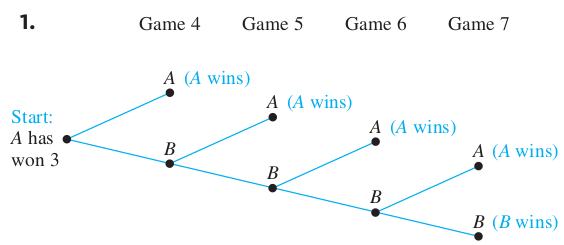
\includegraphics[scale=0.6]{../images/9.2.1.png}
\end{figure}

There are five ways to complete the series: $A$, \(B-A\), \(B-B-A\), \(B-B-B-A\), and \(B-B-B-B\).
\end{proof}

\subsection{Exercise 2}
Suppose team $A$ wins the first two games. How many ways can the World Series be completed? (Draw a tree.)

\begin{proof}
\begin{figure}[ht!]
\centering
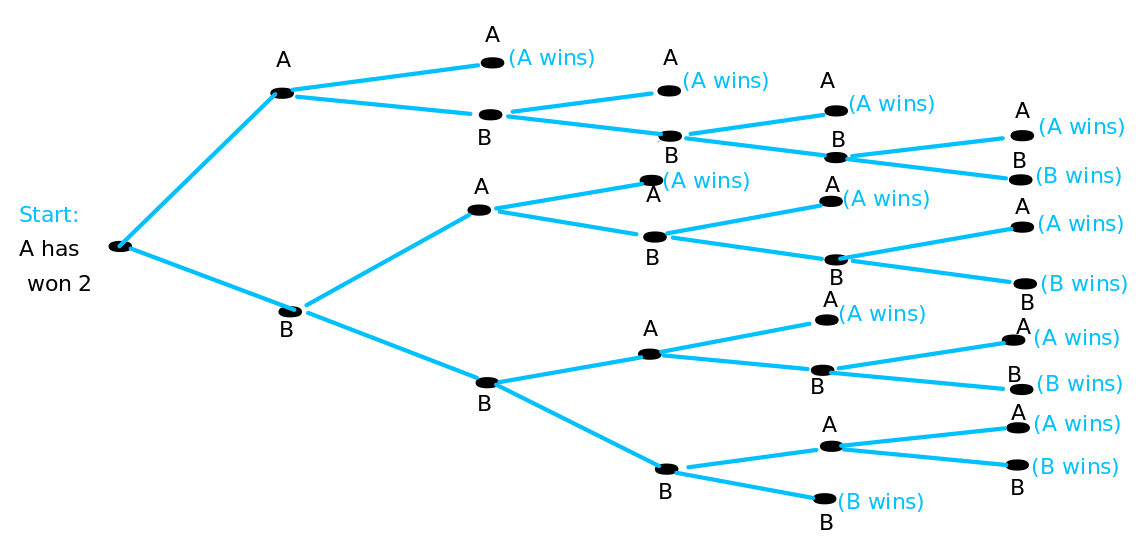
\includegraphics[scale=0.3]{../images/9.2.2.png}
\end{figure}

There are 15 ways: AA, ABA, ABBA, ABBBA, ABBBB, BAA, BABA, BABBA, BABBB, BBAA, BBABA, BBABB, BBBAA, BBBAB, BBBB.
\end{proof}

\subsection{Exercise 3}
How many ways can a World Series be played if team $A$ wins four games in a row?

\begin{proof}
Four ways: \(A-A-A-A, B-A-A-A-A, B-B-A-A-A-A\), and \(B-B-B-A-A-A-A\)
\end{proof}

\subsection{Exercise 4}
How many ways can a World Series be played if no team wins two games in a row?

\begin{proof}
Two ways: \(A-B-A-B-A-B-A\) and \(B-A-B-A-B-A-B\)
\end{proof}

\subsection{Exercise 5}
In a competition between players $X$ and $Y$, the first player to win three games in a row or a total of four games 
wins. How many ways can the competition be played if $X$ wins the first game and $Y$ wins the second and third 
games? (Draw a tree.)

\begin{proof}
\begin{figure}[ht!]
\centering
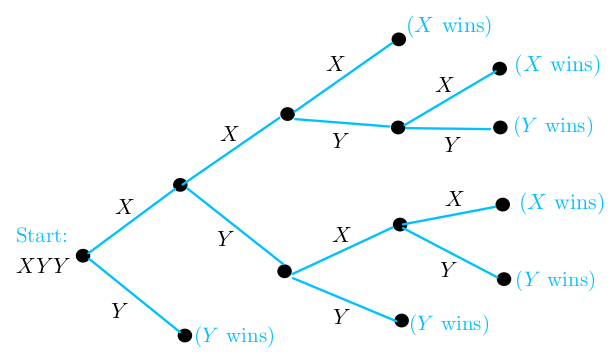
\includegraphics[scale=0.4]{../images/9.2.5.png}
\end{figure}

There are seven ways: \(XXX, XXYX, XXYY, XYXX, XYXY, XYY, Y\).
\end{proof}

\subsection{Exercise 6}
One urn contains two black balls (labeled \(B_1\) and \(B_2\)) and one white ball. A second urn contains one black 
ball and two white balls (labeled \(W_1\) and \(W_2\)). Suppose the following experiment is performed: One of the 
two urns is chosen at random. Next a ball is randomly chosen from the urn. Then a second ball is chosen at random 
from the same urn without replacing the first ball.

\subsubsection{(a)}
Construct the possibility tree showing all possible outcomes of this experiment.

\begin{proof}
\begin{figure}[ht!]
\centering
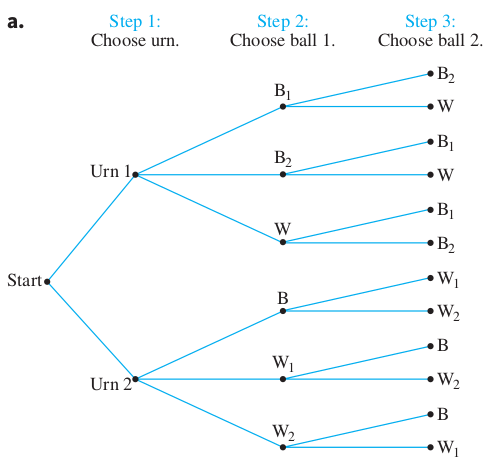
\includegraphics[scale=0.5]{../images/9.2.6.a.png}
\end{figure}
\end{proof}

\subsubsection{(b)}
What is the total number of outcomes of this experiment?

\begin{proof}
12
\end{proof}

\subsubsection{(c)}
What is the probability that two black balls are chosen?

\begin{proof}
\(2/12 = 1/6 \approx 16.6\%\)
\end{proof}

\subsubsection{(d)}
What is the probability that two balls of opposite color are chosen?

\begin{proof}
\(8/12 = 2/3 \approx 66.6\%\)
\end{proof}

\subsection{Exercise 7}
One urn contains one blue ball (labeled \(B_1\)) and three red balls (labeled \(R_1, R_2\), and \(R_3\)). A second urn 
contains two red balls (\(R_4\) and \(R_5\)) and two blue balls (\(B_2\) and \(B_3\)). An experiment is performed in 
which one of the two urns is chosen at random and then two balls are randomly chosen from it, one after the other 
without replacement.

\subsubsection{(a)}
Construct the possibility tree showing all possible outcomes of this experiment.

\begin{proof}
\begin{figure}[ht!]
\centering
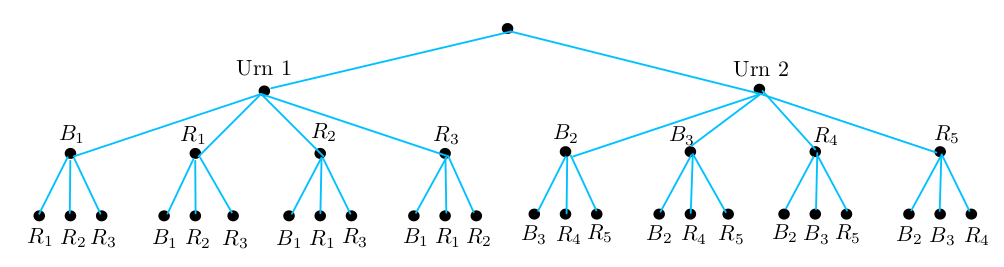
\includegraphics[scale=0.5]{../images/9.2.7.a.png}
\end{figure}
\end{proof}

\subsubsection{(b)}
What is the total number of outcomes of this experiment?

\begin{proof}
24
\end{proof}

\subsubsection{(c)}
What is the probability that two red balls are chosen?

\begin{proof}
\(8/24 = 1/3 \approx 33.3\%\)
\end{proof}

\subsection{Exercise 8}
A person buying a personal computer system is offered a choice of three models of the basic unit, two models of 
keyboard, and two models of printer. How many distinct systems can be purchased?

\begin{proof}
By the multiplication rule, the answer is \(3 \cdot 2 \cdot 2 = 12\).
\end{proof}

\subsection{Exercise 9}
Suppose there are three roads from city $A$ to city $B$ and five roads from city $B$ to city $C$. 

\subsubsection{(a)}
How many ways is it possible to travel from city $A$ to city $C$ via city $B$?

\begin{proof}
In going from city $A$ to city $B$, one may take any of the 3 roads. In going from city $B$ to city $C$, one may take 
any of the 5 roads. So, by the multiplication rule, there are \(3 \cdot 5 = 15\) ways to travel from city $A$ to city 
$C$ via city $B$.
\end{proof}

\subsubsection{(b)}
How many different round-trip routes are there from city $A$ to $B$ to $C$ to $B$ and back to $A$?

\begin{proof}
A round-trip journey can be thought of as a four-step operation: {\cy Step 1:} Go from $A$ to $B$. {\cy Step 2:} 
Go from $B$ to $C$. {\cy Step 3:} Go from $C$ to $B$. {\cy Step 4:} Go from $B$ to $A$.

Since there are 3 ways to perform step 1, 5 ways to perform step 2, 5 ways to perform step 3, and 3 ways to perform 
step 4, by the multiplication rule, there are \(3 \cdot 5 \cdot 5 \cdot 3 = 225\) round-trip routes.
\end{proof}

\subsubsection{(c)}
How many different routes are there from cities $A$ to $B$ to $C$ to $B$ and back to $A$ in which no road is traversed twice?

\begin{proof}
In this case the steps for making a round-trip journey are the same as in part (b), but since no route segment may be 
repeated, there are only 4 ways to perform step 3 and only 2 ways to perform step 4. So, by the multiplication rule, 
there are \(3 \cdot 5 \cdot 4 \cdot 2 = 120\) round-trip routes in which no road is traversed twice.
\end{proof}

\subsection{Exercise 10}
Suppose there are three routes from North Point to Boulder Creek, two routes from Boulder Creek to Beaver Dam, two 
routes from Beaver Dam to Star Lake, and four routes directly from Boulder Creek to Star Lake. (Draw a sketch.)

\subsubsection{(a)}
How many routes from North Point to Star Lake pass through Beaver Dam?

\begin{proof}
By the multiplication rule \(3 \cdot 2 \cdot 2 = 12\) routes.
\end{proof}

\subsubsection{(b)}
How many routes from North Point to Star Lake bypass Beaver Dam?

\begin{proof}
By the multiplication rule \(3 \cdot 4 = 12\) routes.
\end{proof}

\subsection{Exercise 11}
\subsubsection{(a)}
A bit string is a finite sequence of 0’s and 1’s. How many bit strings have length 8?

\begin{proof}
Imagine constructing a bit string of length 8 as an eight-step process:

{\cy Step 1:} Choose either a 0 or a 1 for the left-most position,

{\cy Step 2:} Choose either a 0 or a 1 for the next position to the right.

\(\vdots\)

{\cy Step 8:} Choose either a 0 or a 1 for the right-most position.

Since there are 2 ways to perform each step, the total number of ways to accomplish the entire operation, which is 
the number of different bit strings of length 8, is \(2 \cdot 2 \cdot 2 \cdot 2 \cdot 2 \cdot 2 \cdot 2 \cdot 2 = 
2^8 = 256\).
\end{proof}

\subsubsection{(b)}
How many bit strings of length 8 begin with three 0’s?

\begin{proof}
Imagine that there are three 0’s in the three left-most positions, and imagine filling in the remaining 5 positions 
as a five-step process, where step $i$ is to fill in the \((i + 3)\)rd position. Since there are 2 ways to perform 
each of the 5 steps, there are \(2^5\) ways to perform the entire operation. So there are \(2^5\), or 32, 8-bit 
strings that begin with three 0’s.
\end{proof}

\subsubsection{(c)}
How many bit strings of length 8 begin and end with a 1?

\begin{proof}
\(2^6 = 64\)
\end{proof}

\subsection{Exercise 12}
Hexadecimal numbers are made using the sixteen hexadecimal digits 0, 1, 2, 3, 4, 5, 6, 7, 8, 9, A, B, C, D, E, F and 
are denoted using the subscript 16. For example, 9A2D16 and BC5416 are hexadecimal numbers.

\subsubsection{(a)}
How many hexadecimal numbers begin with one of the digits 3 through B, end with one of the digits 5 through F, and are 
5 digits long?

\begin{proof}
Think of creating a hexadecimal number that satisfies the given requirements as a five-step process. 

{\cy Step 1:} Choose the left-most hexadecimal digits. It can be any of the 9 hexadecimal digits from 3 through B.

{\cy Steps 2-4:} Choose the three hexadecimal digits for the middle three positions. Each can be any of the 16 
hexadecimal digits.

{\cy Step 5:} Choose the right-most hexadecimal digit. It can be any of the 11 hexadecimal digits from 5 through F.

There are 9 ways to perform step 1, 16 ways to perform each of steps 2 through 4, and 11 ways to perform step 5. Thus, 
the total number of specified hexadecimal numbers is \(9 \cdot 16 \cdot 16 \cdot 16 \cdot 11 = 405,504\).
\end{proof}

\subsubsection{(b)}
How many hexadecimal numbers begin with one of the digits 4 through D, end with one of the digits 2 through E, and are 
6 digits long?

\begin{proof}
There are 10 choices for the first digit: 4, 5, 6, 7, 8, 9, A, B, C, D.

There are 14 choices for the first digit: 2, 3, 4, 5, 6, 7, 8, 9, A, B, C, D, E.

There are 16 choices for each one of the 4 middle digits.

So: \(10 \cdot 16 \cdot 16 \cdot 16 \cdot 16 \cdot 14 = 9175040\)
\end{proof}

\subsection{Exercise 13}
A coin is tossed four times. Each time the result H for heads or T for tails is recorded. An outcome of HHTT means that heads were obtained on the first two tosses and tails on the second two. Assume that heads and tails are equally likely on each toss.

\subsubsection{(a)}
How many distinct outcomes are possible?

\begin{proof}
In each of the four tosses there are two possible results: Either a head (H) or a tail (T) is obtained. Thus, by the 
multiplication rule, the number of outcomes is \(2 \cdot 2 \cdot 2 \cdot 2 = 2^4 = 16\).
\end{proof}

\subsubsection{(b)}
What is the probability that exactly two heads occur?

\begin{proof}
There are six outcomes with two heads: HHTT, HTHT, HTTH, THHT, THTH, TTHH. Thus the probability of obtaining exactly 
two heads is \(6/16 = 3/8\).
\end{proof}

\subsubsection{(c)}
What is the probability that exactly one head occurs?

\begin{proof}
There are four outcomes with exactly one head: HTTT, THTT, TTHT, TTTH. Thus the probability of obtaining exactly two 
heads is \(4/16 = 1/4\).
\end{proof}

\subsection{Exercise 14}
Suppose that in a certain state, all automobile license plates have four uppercase letters followed by three 
digits.

\subsubsection{(a)}
How many different license plates are possible?

\begin{proof}
Think of creating license plates that satisfy the given conditions as the following seven-step process: In steps 
1–4 choose the letters to put in positions 1–4, and in steps 5–7, choose the digits to put in positions 5–7. Since 
there are 26 letters and 10 digits and since repetition is allowed, there are 26 ways to perform each of steps 1–4 and 
10 ways to perform each of steps 5–7. Thus the number of license plates is \(26 \cdot 26 \cdot 26 \cdot 26 \cdot 10 
\cdot 10 \cdot 10 = 456,976,000\).
\end{proof}

\subsubsection{(b)}
How many license plates could begin with A and end in 0?
\begin{proof}
In this case there is only one way to perform step 1 (because the first letter must be an A) and only one way to 
perform step 7 (because the last digit must be a 0). Therefore, the number of license plates is 
\(26 \cdot 26 \cdot 26 \cdot 10 \cdot 10 = 1,757,600\).
\end{proof}

\subsubsection{(c)}
How many license plates could begin with TGIF?

\begin{proof}
There are 3 digits left to be chosen. Each has 10 possibilities. So by the multiplication rule \(10^3=1000\)
can begin with TGIF.
\end{proof}

\subsubsection{(d)}
How many license plates are possible in which all the letters and digits are distinct?

\begin{proof}
In this case there are 26 ways to perform step 1, 25 ways to perform step 2, 24 ways to perform step 3, 23 ways to 
perform step 4, 10 ways to perform step 5, 9 ways to perform step 6, and 8 ways to perform step 7, so the number 
of license plates is \(26 \cdot 25 \cdot 24 \cdot 23 \cdot 10 \cdot 9 \cdot 8 = 258,336,000\).
\end{proof}

\subsubsection{(e)}
How many license plates could begin with AB and have all letters and digits distinct?

\begin{proof}
24 choices for the third letter, 23 for the fourth letter. Then 10, 9, 8 choices for the 1st, 2nd, 3rd digits. So:
\(24 \cdot 23 \cdot 10 \cdot 9 \cdot 8 = 397440\).
\end{proof}

\subsection{Exercise 15}
A combination lock requires three selections of numbers, each from 1 through 30.

\subsubsection{(a)}
How many different combinations are possible?

\begin{proof}
\(30^3 = 27000\)
\end{proof}

\subsubsection{(b)}
Suppose the locks are constructed in such a way that no number may be used twice. How many different combinations 
are possible?

\begin{proof}
\(30 \cdot 29 \cdot 28 = 24360\)
\end{proof}

\subsection{Exercise 16}
\subsubsection{(a)}
How many integers are there from 10 through 99?

\begin{proof}
Two solutions:

(i) By the multiplication rule, the number of integers from 10 through 99 = (the number of ways to pick the first 
digit) \(\times\) (the number of ways to pick the second digit) = \(9 \cdot 10 = 90\).

(ii) By Theorem 9.1.1, the number of integers from 10 through 99 = \(90 - 10 + 1 = 90\).
\end{proof}

\subsubsection{(b)}
How many odd integers are there from 10 through 99?

\begin{proof}
Because odd integers end in 1, 3, 5, 7, or 9, the number of odd integers from 10 through 99 = (the number of ways to 
pick the first digit) \(\times\) (the number of ways to pick the second digit) = \(9 \cdot 5 = 45\).

An alternative solution uses the listing method shown in the solution for Example 9.1.4.
\end{proof}

\subsubsection{(c)}
How many integers from 10 through 99 have distinct digits?

\begin{proof}
(the number of ways to pick the first digit) \(\times\) (the number of ways to pick the second digit) = 
\(9 \cdot 9 = 81\).

Another solution is to start with the solution to part (a), which is 90, and subtract the number of integers that have 
the same digit repeated, of which there are 9: 11, 22, 33, 44, 55, 66, 77, 88, 99.
\end{proof}

\subsubsection{(d)}
How many odd integers from 10 through 99 have distinct digits?

\begin{proof}
(the number of ways to pick the second digit) \(\times\) (the number of ways to pick the first digit) = \(5 \cdot 8 
= 40\). Here the second digit can be 1,3,5,7,9; and the first digit cannot be 0 or the same as the first digit.
\end{proof}

\subsubsection{(e)}
What is the probability that a randomly chosen two-digit integer has distinct digits? has distinct digits and is odd?

\begin{proof}
81/90 = 9/10, 40/90 = 4/9
\end{proof}

\subsection{Exercise 17}
\subsubsection{(a)}
How many integers are there from 1000 through 9999?

\begin{proof}
By Theorem 9.1.1, \(9999-1000+1 = 9000\). Another solution: there are 9 choices for the first digit (cannot be 0), and
10 choices for the other 3 digits, so \(9 \cdot 10 \cdot 10 \cdot 10 = 9000\).
\end{proof}

\subsubsection{(b)}
How many odd integers are there from 1000 through 9999?

\begin{proof}
4500.

One solution is that it's half of the answer to part (a), since half the integers are even, and the other odd. 

Another solution: there are 9 choices for the first digit (cannot be 0), 10 choices for the second and third digits,
and 5 choices for the last (1,3,5,7,9), therefore \(9 \cdot 10 \cdot 10 \cdot 5 = 4500\).
\end{proof}

\subsubsection{(c)}
How many integers from 1000 through 9999 have distinct digits?

\begin{proof}
There are 9 choices for the first digit (cannot be 0). There are 9 choices for the second digit (cannot be the same as the first digit, but can be 0). Then 8 and 7 choices for the third and fourth digits. So there are  
\(9 \cdot 9 \cdot 8 \cdot 7 = 4536\) such integers.
\end{proof}

\subsubsection{(d)}
How many odd integers from 1000 through 9999 have distinct digits?

\begin{proof}
There are 5 choices for the last digit (1, 3, 5, 7, 9). There are 8 choices for the first digit (cannot be the 
same as the last digit, and cannot be 0). Then 8 choices for the second digit (cannot be the same as the first or 
the last, but can be 0) and 7 choices for the third digit. So there are \(5 \cdot 8 \cdot 8 \cdot 7 = 2240\) such 
integers.
\end{proof}

\subsubsection{(e)}
What is the probability that a randomly chosen four-digit integer has distinct digits? has distinct digits and is odd?

\begin{proof}
4536/9000, 2240/9000
\end{proof}

\subsection{Exercise 18}
The following diagram shows the keypad for an automatic teller machine. As you can see, the same sequence of keys 
represents a variety of different PINs. For instance, 2133, AZDE, and BQ3F are all keyed in exactly the same way.

\begin{figure}[ht!]
\centering
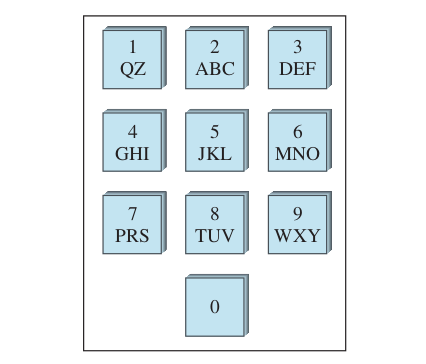
\includegraphics[scale=0.5]{../images/9.2.18.png}
\end{figure}

\subsubsection{(a)}
How many different PINs are represented by the same sequence of keys as 2133?

\begin{proof}
Let step 1 be to choose either the number 2 or one of the letters corresponding to the number 2 on the keypad, let 
step 2 be to choose either the number 1 or one of the letters corresponding to the number 1 on the keypad, and 
let steps 3 and 4 be to choose either the number 3 or one of the letters corresponding to the number 3 on the keypad. 
There are 4 ways to perform step 1, 3 ways to perform step 2, and 4 ways to perform each of steps 3 and 4. So by the 
multiplication rule, there are \(4 \cdot 3 \cdot 4 \cdot 4 = 192\) ways to perform the entire operation. Thus there 
are 192 different PINs that are keyed the same as 2133. Note that on a computer keyboard, these PINs would not be 
keyed the same way.
\end{proof}

\subsubsection{(b)}
How many different PINs are represented by the same sequence of keys as 5031?

\begin{proof}
\(4 \cdot 1 \cdot 4 \cdot 3 = 48\)
\end{proof}

\subsubsection{(c)}
How many different numeric sequences on the machine contain no repeated digit?

\begin{proof}
\(10 \cdot 9 \cdot 8 \cdot 7 = 5040\)
\end{proof}

\subsection{Exercise 19}
Three officers - a president, a treasurer, and a secretary - are to be chosen from among four people: Ann, Bob, Cyd, 
and Dan. Suppose that Bob is not qualified to be treasurer and Cyd’s other commitments make it impossible for her to 
be secretary. How many ways can the officers be chosen? Can the multiplication rule be used to solve this problem?

\begin{proof}
There are 14 different paths from “root” to “leaf” of this possibility tree, and so there are 14 ways the officers can 
be chosen. Because \(14 = 2\cdot7\), reordering the steps will not make it possible to use the multiplication rule 
alone to solve this problem.

\begin{figure}[ht!]
\centering
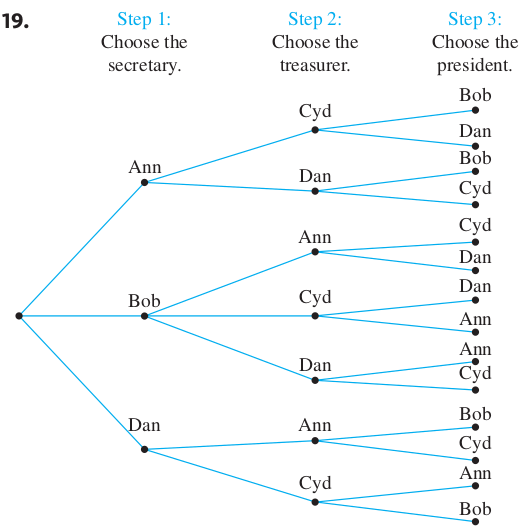
\includegraphics[scale=0.45]{../images/9.2.19.png}
\end{figure}
\end{proof}

\subsection{Exercise 20}
Modify Example 9.2.2 by supposing that a PIN must not begin with any of the letters A-M and must end with a digit. Continue to assume that no symbol may be used more than once and that the total number of PINs is to be determined.

\subsubsection{(a)}
Find the error in the following “solution.” “Constructing a PIN is a four-step process. 

Step 1: Choose the left-most symbol.

Step 2: Choose the second symbol from the left.

Step 3: Choose the third symbol from the left.

Step 4: Choose the right-most symbol.

Because none of the thirteen letters from A through M may be chosen in step 1, there are \(36 - 13 = 23\) ways to 
perform step 1. There are 35 ways to perform step 2 and 34 ways to perform step 3 because previously used symbols may 
not be used. Since the symbol chosen in step 4 must be a previously unused digit, there are \(10 - 3 = 7\) ways to 
perform step 4. Thus there are \(23 \cdot 35 \cdot 34 \cdot 7 = 191,590\) different PINs that satisfy the given 
conditions.”

\begin{proof}
The number of ways to perform step 4 is not constant; it depends on how the previous steps were performed. For 
instance, if 3 digits had been chosen in steps 1-3, then there would be \(10 - 3 = 7\) ways to perform step 4, but 
if 3 letters had been chosen in steps 1-3, then there would be 10 ways to perform step 4.
\end{proof}

\subsubsection{(b)}
Reorder steps 1-4 in part (a) as follows: {\cy Step 1:} Choose the right-most symbol. {\cy Step 2:} Choose the 
left-most symbol. {\cy Step 3:} Choose the second symbol from the left. {\cy Step 4:} Choose the third symbol from 
the left. Use the multiplication rule to find the number of PINs that satisfy the given conditions.

\begin{proof}
\(10 \cdot 22 \cdot 34 \cdot 33 = 246840\)
\end{proof}

\subsection{Exercise 21}
Suppose $A$ is a set with $m$ elements and $B$ is a set with $n$ elements.

\subsubsection{(a)}
How many relations are there from $A$ to $B$? Explain.

\begin{proof}
\(2^{mn}\). There are $mn$ pairs in \(A \times B\). A relation is simply any subset of \(A \times B\). So the
number of relations from $A$ to $B$ is the same as the size of the power set of \(A \times B\), which is \(2^{mn}\).
\end{proof}

\subsubsection{(b)}
How many functions are there from $A$ to $B$? Explain.

\begin{proof}
\(n^m\). For each input \(a \in A\) there are $n$ possible outputs \(b \in B\). Since there are $m$ inputs, by the
multiplication rule there are \(n \cdot n \cdots n = n^m\) functions.
\end{proof}

\subsubsection{(c)}
What fraction of the relations from $A$ to $B$ are functions?

\begin{proof}
\(n^m / 2^{mn}\)
\end{proof}

\subsection{Exercise 22}
\subsubsection{(a)}
How many functions are there from a set with three elements to a set with four elements?

\begin{proof}
The answer is \(4 \cdot 4 \cdot 4 = 4^3 = 64\). Imagine creating a function from a 3-element set to a 4-element set 
as a three-step process: Step 1 is to send the first element of the 3-element set to an element of the 4-element 
set (there are four ways to perform this step); step 2 is to send the second element of the 3-element set to an 
element of the 4-element set (there are also four ways to perform this step); and step 3 is to send the third element 
of the 3-element set to an element of the 4-element set (there are four ways to perform this step). Thus the entire 
process can be performed in \(4 \cdot 4 \cdot 4\) different ways.
\end{proof}

\subsubsection{(b)}
How many functions are there from a set with five elements to a set with two elements?

\begin{proof}
\(2^5 = 32\)
\end{proof}

\subsubsection{(c)}
How many functions are there from a set with $m$ elements to a set with $n$ elements, where $m$ and $n$ are positive 
integers?

\begin{proof}
\(n^m\).
\end{proof}

\subsection{Exercise 23}
In Section 2.5 we showed how integers can be represented by strings of 0’s and 1’s inside a digital computer. In fact, 
through various coding schemes, strings of 0’s and 1’s can be used to represent all kinds of symbols. One commonly 
used code is the Extended Binary-Coded Decimal Interchange Code (EBCDIC) in which each symbol has an 8-bit 
representation. How many distinct symbols can be represented by this code?

\begin{proof}
\(2^8 = 256\)
\end{proof}

{\bf \cy In each of $24-28$, determine how many times the innermost loop will be iterated when the algorithm segment 
is implemented and run. (assume that \(m, n, p, a, b, c\), and $d$ are all positive integers.)}

\subsection{Exercise 24}
\begin{tabbing}
{\bf for} \= \(i \coloneqq 1\) {\bf to} 30 \\
          \> {\bf for} \= \(j \coloneqq 1\) {\bf to} 15 \\
          \>           \> {\it [Statements in body of inner loop.]} \\
          \>           \> {\it [None contain branching statements that lead outside the loop.]} \\
          \> {\bf next j} \\
{\bf next i}
\end{tabbing}

\begin{proof}
The outer loop is iterated 30 times, and during each iteration of the outer loop there are 15 iterations of the 
inner loop. Hence, by the multiplication rule, the total number of iterations of the inner loop is 
\(30 \cdot 15 = 450\).
\end{proof}

\subsection{Exercise 25}
\begin{tabbing}
{\bf for} \= \(j \coloneqq 1\) {\bf to} $m$ \\
          \> {\bf for} \= \(k \coloneqq 1\) {\bf to} $n$ \\
          \>           \> {\it [Statements in body of inner loop.]} \\
          \>           \> {\it [None contain branching statements that lead outside the loop.]} \\
          \> {\bf next k} \\
{\bf next j}
\end{tabbing}

\begin{proof}
\(mn\)
\end{proof}

\subsection{Exercise 26}
\begin{tabbing}
{\bf for} \= \(i \coloneqq 1\) {\bf to} $m$ \\
          \> {\bf for} \= \(j \coloneqq 1\) {\bf to} $n$ \\
          \>           \> {\bf for} \= \(k \coloneqq 1\) {\bf to} $p$ \\
          \>           \>           \> {\it [Statements in body of inner loop.]} \\
          \>           \>           \> {\it [None contain branching statements that lead outside the loop.]} \\
          \>           \> {\bf next k} \\
          \> {\bf next j} \\
{\bf next i}
\end{tabbing}

\begin{proof}
\(mnp\)
\end{proof}

\subsection{Exercise 27}
\begin{tabbing}
{\bf for} \= \(i \coloneqq 5\) {\bf to} 50 \\
          \> {\bf for} \= \(j \coloneqq 10\) {\bf to} 20 \\
          \>           \> {\it [Statements in body of inner loop.]} \\
          \>           \> {\it [None contain branching statements that lead outside the loop.]} \\
          \> {\bf next j} \\
{\bf next i}
\end{tabbing}

\begin{proof}
The outer loop is iterated \(50 - 5 + 1 = 46\) times, and during each iteration of the outer loop there are 
\(20 - 10 + 1 = 11\) iterations of the inner loop. Hence, by the multiplication rule, the total number of iterations 
of the inner loop is \(46 \cdot 11 = 506\).
\end{proof}

\subsection{Exercise 28}
Assume \(a \leq b\) and \(c \leq d\).
\begin{tabbing}
{\bf for} \= \(i \coloneqq a\) {\bf to} $b$ \\
          \> {\bf for} \= \(j \coloneqq c\) {\bf to} $d$ \\
          \>           \> {\it [Statements in body of inner loop.]} \\
          \>           \> {\it [None contain branching statements that lead outside the loop.]} \\
          \> {\bf next j} \\
{\bf next i}
\end{tabbing}

\begin{proof}
\((b-a+1)(d-c+1)\)
\end{proof}

\subsection{Exercise 29}
Consider the numbers 1 through 99,999 in their ordinary decimal representations. How many contain exactly one of 
each of the digits 2, 3, 4, and 5?

{\it Hint:} An efficient solution is to add leading zeros as needed to make each number five digits long. For 
instance, write 1 as 00001. Then, instead of choosing digits for the positions, choose positions for the digits. 
The answer is 720.

\begin{proof}
Following the Hint, there are 5 possible positions to place 2, then 4 positions to place 3, 3 positions to place 4, 2
positions to place 5, and 6 choices for the last position (1, 6, 7, 8, 9, 0). Therefore \(5 \cdot 4 \cdot 3 \cdot 2
\cdot 6 = 720\). (Notice that there is no issue with the digit 0, since it can be placed in the first position.)
\end{proof}

\subsection{Exercise 30}
Let \(n = p_1^{k_1} p_2^{k_2} \cdots p_m^{k_m}\) where \(p_1, p_2, \ldots, p_m\) are distinct prime numbers and 
\(k_1, k_2, \ldots, k_m\) are positive integers. How many ways can $n$ be written as a product of two positive 
integers that have no common factors, assuming the following?

\subsubsection{(a)}
Order matters (that is, \(8 \cdot 15\) and \(15 \cdot 8\) are regarded as different).

\begin{proof}
To split $n$ into two positive integers $a, b$ that have no common factors, we need to split the set of all the prime 
powers \(\{p_1^{k_1}, \cdots, p_m^{k_m}\) into two disjoint subsets $A, B$. Then $a$ is the product of the prime powers in $A$, and $b$ is the product of those in $B$.

When one of the subsets is chosen, the other is automatically forced to be what's left. For example, if the
set is \(p_1^{k_1}, p_2^{k_2}, p_3^{k_3}\) and we choose $A$ to be \(\{p_1^{k_1}, p_3^{k_3}\}\) then $B$ has to be
\(\{p_2^{k_2}\}\).

However, since order matters, choosing $A$ to be \(\{p_1^{k_1}, p_3^{k_3}\}\) and $B$ to be \(\{p_2^{k_2}\}\) 
is considered different than choosing $A$ to be \(\{p_2^{k_2}\}\) and $B$ to be \(\{p_1^{k_1}, p_3^{k_3}\}\).

This means that the number of ways to write $n$ as the product of two positive integers with no common prime 
factors is equal to the number of ways we can choose $A$ to be a subset of \(\{p_1^{k_1}, \ldots, p_m^{k_m}\}\). This 
is a set with $m$ elements, so it has $2^m$ subsets. So there are $2^m$ ways to choose $A$, which is the answer.
\end{proof}

\subsubsection{(b)}
Order does not matter (that is, \(8 \cdot 15\) and \(15 \cdot 8\) are regarded as the same).

\begin{proof}
The solution is the same as in part (a) except the choices where $A$ and $B$ are swapped do not count. For example, 
choosing $A$ to be \(\{p_1^{k_1}, p_3^{k_3}\}\) and $B$ to be \(\{p_2^{k_2}\}\) is considered the same as choosing $A$ 
to be \(\{p_2^{k_2}\}\) and $B$ to be \(\{p_1^{k_1}, p_3^{k_3}\}\).

So, in this case the answer is half the answer to part (a), namely, \(2^m / 2 = 2^{m-1}\).
\end{proof}

\subsection{Exercise 31}
\subsubsection{(a)}
If $p$ is a prime number and $a$ is a positive integer, how many distinct positive divisors does $p^a$ have?

\begin{proof}
There are \(a + 1\) divisors: \(1, p, p^2, \ldots, p^a\).
\end{proof}

\subsubsection{(b)}
If $p$ and $q$ are distinct prime numbers and $a$ and $b$ are positive integers, how many distinct positive divisors 
does $p^a q^b$ have?

\begin{proof}
A divisor is a product of any one of the \(a + 1\) numbers listed in part (a) times any one of the \(b + 1\) numbers 
\(1, q, q^2, \ldots, q^b\). So, by the multiplication rule, there are \((a + 1)(b + 1)\) divisors in all.
\end{proof}

\subsubsection{(c)}
If $p, q$, and $r$ are distinct prime numbers and $a, b$, and $c$ are positive integers, how many distinct positive 
divisors does $p^a q^b r^c$ have?

\begin{proof}
\((a+1)(b+1)(c+1)\)
\end{proof}

\subsubsection{(d)}
If \(p_1, p_2, \ldots, p_m\) are distinct prime numbers and \(a_1, a_2, \ldots, a_m\) are positive integers, how many 
distinct positive divisors does \(p_1^{a_1} p_2^{a_2} \cdots p_m^{a_m}\) have?

\begin{proof}
\((a_1+1)(a_2+1) \cdots (a_m+1)\)
\end{proof}

\subsubsection{(e)}
What is the smallest positive integer with exactly 12 divisors?

\begin{proof}
Assume \(p_1, p_2, \ldots, p_m\) are distinct prime numbers and \(a_1, a_2, \ldots, a_m\) are positive integers, and 
\(n = p_1^{a_1} p_2^{a_2} \cdots p_m^{a_m}\) is the integer we are looking for. Assume $n$ has exactly 12 divisors.

By part (d), \(12 = 2 \cdot 2 \cdot 3\) so $m=3$ and \(2 \cdot 2 \cdot 3 = (a_1+1)(a_2+1)(a_3+1)\) so it follows 
\(a_1 = 1, a_2 = 1, a_3 = 2\). 

To make $n$ as small as possible, we can choose the smallest first three primes 2, 3, 5, and since \(a_3 = 2\) 
we can let \(p_1 = 3, p_2 = 5, p_3 = 2\). (This way the highest power 2 goes on top of the smallest base prime, 2.)

Therefore \(n = p_1^{a_1} p_2^{a_2} p_3^{a_3} = 3^1 \cdot 5^1 \cdot 2^2 = 60\) is the smallest positive integer with 
exactly 12 divisors: 1, 2, 3, 4, 5, 6, 10, 12, 15, 20, 30, 60.
\end{proof}

\subsection{Exercise 32}
\subsubsection{(a)}
How many ways can the letters of the word ALGORITHM be arranged in a row?

\begin{proof}
Since the nine letters of the word ALGORITHM are all distinct, there are as many arrangements of these letters 
in a row as there are permutations of a set with nine elements: \(9! = 362,880\).
\end{proof}

\subsubsection{(b)}
How many ways can the letters of the word ALGORITHM be arranged in a row if A and L must remain together (in 
order) as a unit?

\begin{proof}
In this case there are effectively eight symbols to be permuted (because AL may be regarded as a single symbol). 
So the number of arrangements is \(8! = 40,320\).
\end{proof}

\subsubsection{(c)}
How many ways can the letters of the word ALGORITHM be arranged in a row if the letters GOR must remain together 
(in order) as a unit?

\begin{proof}
In this case there are effectively seven symbols to be permuted (because GOR may be regarded as a single symbol). 
So the number of arrangements is \(7! = 5040\).
\end{proof}

\subsection{Exercise 33}
Six people attend the theater together and sit in a row with exactly six seats.

\subsubsection{(a)}
How many ways can they be seated together in the row?

\begin{proof}
\(6! = 720\)
\end{proof}

\subsubsection{(b)}
Suppose one of the six is a doctor who must sit on the aisle in case she is paged. How many ways can the people be 
seated together in the row with the doctor in an aisle seat?

\begin{proof}
Excluding the doctor who must sit on the aisle seat, \(5! = 120\) ways. (However the question is a bit ambiguous, are 
there 2 aisle seats, one on each side of the row? In that case the answer would be 240.)
\end{proof}

\subsubsection{(c)}
Suppose the six people consist of three married couples and each couple wants to sit together with the older partner on 
the left. How many ways can the six be seated together in the row?

\begin{proof}
The couples can be treated as one person, so \(3! = 6\).
\end{proof}

\subsection{Exercise 34}
Five people are to be seated around a circular table. Two seatings are considered the same if one is a rotation of 
the other. How many different seatings are possible?

\begin{proof}
The same reasoning as in Example 9.2.9 gives an answer of \(4! = 24\).
\end{proof}

\subsection{Exercise 35}
Write all the 2-permutations of \(\{W, X, Y, Z\}\).

\begin{proof}
\(WX, WY, WZ, XW, XY, XZ, YW, YX, YZ, ZW, ZX, ZY\)
\end{proof}

\subsection{Exercise 36}
Write all the 3-permutations of \(\{s, t, u, v\}\).

\begin{proof}
There are \(P(4,3) = \dps\frac{4!}{(4-3)!} = 24\) 3-permutations of a 4-element set. So:

\(stu, stv, suv, sut, svt, svu, tsu, tsv, tuv, tus, tvs, tvu,\)

\(ust, usv, utv, uts, uvs, uvt, vst, vsu, vtu, vts, vus, vut.\)
\end{proof}

\subsection{Exercise 37}
Evaluate the following quantities.

\subsubsection{(a)}
\(P(6, 4)\)
\begin{proof}
\(P(6,4) = \dps\frac{6!}{(6-4)!} = \frac{6!}{2!} = \frac{6 \cdot 5 \cdot 4 \cdot 3 \cdot \Ccancel[cyan]{2 \cdot 1}}
{\Ccancel[cyan]{2 \cdot 1}} = 360\)
\end{proof}

\subsubsection{(b)}
\(P(6, 6)\)
\begin{proof}
\(P(6,6) = \dps\frac{6!}{(6-6)!} = \frac{6!}{0!} = 720/1 = 720\)
\end{proof}

\subsubsection{(c)}
\(P(6, 3)\)
\begin{proof}
\(P(6,3) = \dps\frac{6!}{(6-3)!} = \frac{6!}{3!} = \frac{6 \cdot 5 \cdot 4 \cdot \Ccancel[cyan]{3 \cdot 2 \cdot 1}}
{\Ccancel[cyan]{3 \cdot 2 \cdot 1}} = 120\)
\end{proof}

\subsubsection{(d)}
\(P(6, 1)\)
\begin{proof}
\(P(6,1) = \dps\frac{6!}{(6-1)!} = \frac{6!}{5!} = \frac{6 \cdot \Ccancel[cyan]{5 \cdot 4 \cdot 3 \cdot 2 \cdot 1}}
{\Ccancel[cyan]{5 \cdot 4 \cdot 3 \cdot 2 \cdot 1}} = 6\)
\end{proof}

\subsection{Exercise 38}
\subsubsection{(a)}
How many 3-permutations are there of a set of five objects?

\begin{proof}
\(P(5,3) = \dps\frac{5!}{(5-3)!} = \frac{5!}{2!} = \frac{5 \cdot 4 \cdot 3 \cdot \Ccancel[cyan]{2 \cdot 1}}
{\Ccancel[cyan]{2 \cdot 1}} = 60\)
\end{proof}

\subsubsection{(b)}
How many 2-permutations are there of a set of eight objects?

\begin{proof}
\(P(8,2) = \dps\frac{8!}{(8-2)!} = \frac{8!}{6!} = \frac{8 \cdot 7 \cdot \Ccancel[cyan]{6 \cdot 5 \cdot 4 \cdot 3 
\cdot 2 \cdot 1}}{\Ccancel[cyan]{6 \cdot 5 \cdot 4 \cdot 3 
\cdot 2 \cdot 1}} = 56\)
\end{proof}

\subsection{Exercise 39}
\subsubsection{(a)}
How many ways can three of the letters of the word ALGORITHM be selected and written in a row?

\begin{proof}
\(P(9,3) = \dps\frac{9!}{(9-3)!} = \frac{9!}{6!} = \frac{9 \cdot 8 \cdot 7 \cdot \Ccancel[cyan]{6!}}
{\Ccancel[cyan]{6!}} = 504\)
\end{proof}

\subsubsection{(b)}
How many ways can six of the letters of the word ALGORITHM be selected and written in a row?

\begin{proof}
\(P(9,6) = \dps\frac{9!}{(9-6)!} = \frac{9!}{3!} = \frac{9 \cdot 8 \cdot 7 \cdot 6 \cdot 5 \cdot 4 \cdot 
\Ccancel[cyan]{3!}}{\Ccancel[cyan]{3!}} = 60480\)
\end{proof}

\subsubsection{(c)}
How many ways can six of the letters of the word ALGORITHM be selected and written in a row if the first letter must be A?

\begin{proof}
\(P(8,5) = \dps\frac{8!}{(8-5)!} = \frac{8!}{3!} = \frac{8 \cdot 7 \cdot 6 \cdot 5 \cdot 4 \cdot \Ccancel[cyan]{3!}}
{\Ccancel[cyan]{3!}} = 6720\)
\end{proof}

\subsubsection{(d)}
How many ways can six of the letters of the word ALGORITHM be selected and written in a row if the first two letters must be OR?

\begin{proof}
\(P(7,4) = \dps\frac{7!}{(7-4)!} = \frac{7!}{3!} = \frac{7 \cdot 6 \cdot 5 \cdot 4 \cdot \Ccancel[cyan]{3!}}
{\Ccancel[cyan]{3!}} = 840\)
\end{proof}

\subsection{Exercise 40}
Prove that for every integer \(n \geq 2\), \(P(n + 1, 3) = n^3 - n\).

\begin{proof}
\(P(n+1,3) = \dps\frac{(n+1)!}{(n+1-3)!} = \frac{(n+1)!}{(n-2)!} = \frac{(n+1) \cdot n \cdot (n-1) \cdot 
\Ccancel[cyan]{(n-2)!}}{\Ccancel[cyan]{(n-2)!}}\)

\(= (n+1)n(n-1) = (n^2-1)n = n^3-n\)
\end{proof}

\subsection{Exercise 41}
Prove that for every integer \(n \geq 2\), \(P(n + 1, 2) - P(n, 2) = 2P(n, 1)\).

\begin{proof}
\(P(n+1,2) = \dps\frac{(n+1)!}{(n+1-2)!} = \frac{(n+1)!}{(n-1)!} = \frac{(n+1) \cdot n!}{(n-1)!} = (n+1)P(n,1)\)

\(P(n,2) = \dps\frac{n!}{(n-2)!} = \frac{(n-1) \cdot n!}{(n-1) \cdot (n-2)!} = (n-1)\frac{n!}{(n-1)!}=(n-1)P(n,1)\)

So \(P(n + 1, 2) - P(n, 2) = (n+1)P(n, 1) - (n-1)P(n, 1) = 2P(n,1)\).
\end{proof}

\subsection{Exercise 42}
Prove that for every integer \(n \geq 3\), \(P(n + 1, 3) - P(n, 3) = 3P(n, 2)\).

\begin{proof}
\(P(n+1,3) = \dps\frac{(n+1)!}{(n+1-3)!} = \frac{(n+1)!}{(n-2)!} = \frac{(n+1) \cdot n!}{(n-2)!} = (n+1)P(n,2)\)

\(P(n,3) = \dps\frac{n!}{(n-3)!} = \frac{(n-2) \cdot n!}{(n-2) \cdot (n-3)!} = (n-2)\frac{n!}{(n-2)!}=(n-2)P(n,2)\)

So \(P(n + 1, 3) - P(n, 3) = (n+1)P(n, 2) - (n-2)P(n, 2) = 3P(n,2)\).
\end{proof}

\subsection{Exercise 43}
Prove that for every integer \(n \geq 2\), \(P(n, n) = P(n, n - 1)\).

\begin{proof}
\(P(n,n)= \dps\frac{n!}{(n-n)!} = \frac{n!}{0!} = \frac{n!}{1} = \frac{n!}{1!} = \frac{n!}{(n-(n-1))!} = P(n,n-1)\)
\end{proof}

\subsection{Exercise 44}
Prove Theorem 9.2.1 by mathematical induction.

\begin{proof}
Let \(P(k)\) be the statement: ``If an operation consists of $k$ steps and the first step can be performed in $n_1$ 
ways, the second step can be performed in $n_2$ ways {\it [regardless of how the first step was performed]}, 
\(\ldots\), the $k$th step can be performed in $n_k$ ways {\it [regardless of how the preceding steps were 
performed]}, then the entire operation can be performed in \(n_1n_2 \cdots n_k\) ways.''

{\bf Show that \(P(1)\) is true:} Assume an operation consists of 1 step, and the first step can be performed in
\(n_1\) ways. Then the whole operation can be performed in \(n_1\) ways, so \(P(1)\) is true.

{\bf Show that for any integer \(k \geq 1\) if \(P(k)\) is true then \(P(k+1)\) is true:} Assume an operation consists
of $k+1$ steps, and assume steps \(1, 2, 3, \ldots, k+1\) can be performed in \(n_1, n_2, \ldots, n_{k+1}\) ways,
respectively, regardless of how preceding steps are performed. Assume that the first $k$ steps can be performed 
in \(n_1n_2 \cdots n_k\) ways. {\it [This is the inductive hypothesis.]}

Since the $k+1$st step can be performed in \(n_{k+1}\) ways regardless of how the preceding $k$ steps were performed, 
for each way of performing the preceding $k$ steps, there are \(n_{k+1}\) ways to perform step $k+1$. Thus there are
\[
\underbrace{n_{k+1} + n_{k+1} + \cdots + n_{k+1}}_{n_1n_2 \cdots n_k \text{ times}}
\]
ways to perform the whole task, where the sum has \(n_1n_2 \cdots n_k\) terms. And the sum equals
\[
n_{k+1} \cdot (n_1n_2 \cdots n_k) = n_1n_2 \cdots n_k n_{k+1}
\]
{\it [as was to be shown.]}
\end{proof}

\subsection{Exercise 45}
Prove Theorem 9.2.2 by mathematical induction.

\begin{proof}
Let \(P(n)\) be the statement ``For any integer $n$ with \(n \geq 1\), the number of permutations of a set with $n$ 
elements is \(n!\).''

{\bf Show that \(P(1)\) is true:} There is only 1 permutation of a set with 1 element, and \(1! = 1\), so 
\(P(1)\) is true.

{\bf Show that for any integer \(k \geq 1\) if \(P(k)\) is true then \(P(k+1)\) is true:} Assume \(k \geq 1\) and 
assume that the number of permutations of any set with $k$ elements is $k!$. {\it [This is the inductive hypothesis.]}
Assume \(A = \{a_1, \ldots, a_{k+1}\}\) is a set with $k+1$ elements.

Consider the subset \(A' = \{a_1, \ldots, a_k\}\) of $A$ with $k$ elements. By the inductive hypothesis $A'$ has 
$k!$ permutations. Now we need to find a way to write the permutations of $A$ in terms of the permutations of $A'$.

Every permutation of $A$ can be thought of as taking a permutation of $A$ and then inserting \(a_{k+1}\) into a
position in that permutation. For example, if \(a_3, a_1, a_{k-2}, \ldots, a_k, a_2, a_{k-1}\) is a permutation of 
$A'$, then there are $k+1$ positions in which \(a_{k+1}\) can be inserted to obtain a permutation of $A$:
\begin{center}
\begin{tabular}{ccccccccccccccc}
& \(a_3\) & & \(a_1\) & & \(a_{k-2}\) & & \(\ldots\) & & \(a_k\) & & \(a_2\) & & \(a_{k-1}\) & \\
\(\uparrow\) & & \(\uparrow\) & & \(\uparrow\) & & \(\uparrow\)& \(\ldots\) & \(\uparrow\) & & \(\uparrow\)& &\(\uparrow\)& & \(\uparrow\) \\
here & & here & & here & & here& \(\ldots\) & here & & here& &here& & here \\
\end{tabular}
\end{center}
So for each permutation of $A'$, there are $k+1$ permutations of $A$. Therefore the number of permutations 
of $A$ is \(k! \cdot (k+1) = (k+1)!\).
\end{proof}

\subsection{Exercise 46}
Prove Theorem 9.2.3 by mathematical induction.

\begin{proof}
Let \(Q(n)\) be the statement: ``for every integer $r$ with \(1 \leq r \leq n\), 
\(P(n,r) = n(n - 1)(n - 2) \cdots (n - r + 1)\).''

{\bf Show that \(Q(1)\) is true:} There is only one 1-permutation of a set of 1 element, and when \(n=r=1\)
the formula \(n(n - 1)(n - 2) \cdots (n - r + 1)\) is equal to 1. Therefore \(Q(1)\) is true.

{\bf Show that for any integer \(k \geq 1\) if \(Q(k)\) is true then \(Q(k+1)\) is true:} Assume \(k \geq 1\) and 
assume for every integer $r$ with \(1 \leq r \leq k\), \(P(k,r) = k(k - 1)(k - 2) \cdots (k - r + 1)\). 
{\it [This is the inductive hypothesis.]}

We want to show that for every integer $r$ with \(1 \leq r \leq k+1\), \(P(k+1,r) = (k+1)k(k-1) \cdots (k-r + 2)\).

When \(r = 1\), there are $k+1$ ways to choose 1 element from a set of $k+1$ elements. So \(P(k+1,1) = k+1\), and
the formula \((k+1)k(k-1) \cdots (k-r + 2)\) for \(r = 1\) becomes \((k+1)\), therefore the formula holds.

Now assume \(2 \leq r \leq k+1\). We can think of choosing $r$ elements from a set of $k+1$ elements as follows: first
choosing 1 element out of $k+1$ elements, then choosing $r-1$ elements from the remaining $k$ elements.

There are $k+1$ ways to choose the first element. Then by the inductive hypothesis there are \(P(k, r-1) = k(k - 1)
(k - 2) \cdots (k - (r-1) + 1) = k(k - 1)(k - 2) \cdots (k - r + 2)\) ways to choose $r-1$ elements from the remaining
$k$ elements. Then by the multiplication rule, \(P(k+1,r) = (k+1) \cdot k(k - 1)(k - 2) \cdots (k - r + 2)\), 
{\it [as was to be shown.]}
\end{proof}

\subsection{Exercise 47}
A permutation on a set can be regarded as a function from the set to itself. For instance, one permutation of 
\(\{1, 2, 3, 4\}\) is 2341. It can be identified with the function that sends each position number to the number 
occupying that position. Since position 1 is occupied by 2, 1 is sent to 2 or \(1 \to 2\); since position 2 is occupied 
by 3, 2 is sent to 3 or \(2 \to 3\); and so forth. The entire permutation can be written using arrows as follows:

\begin{center}
\begin{tabular}{cccc}
1&2&3&4 \\
\cyda & \cyda & \cyda & \cyda \\
2&3&4&1 \\
\end{tabular}
\end{center}

\subsubsection{(a)}
Use arrows to write each of the six permutations of \(\{1, 2, 3\}\).

\begin{proof}
\begin{center}
\begin{tabular}{ccc|ccc|ccc|ccc|ccc|ccc}
1&2&3&1&2&3&1&2&3&1&2&3&1&2&3&1&2&3 \\
\cyda & \cyda & \cyda & \cyda & \cyda & \cyda & \cyda & \cyda & \cyda & \cyda & \cyda & \cyda & \cyda & \cyda & 
\cyda & \cyda & \cyda & \cyda \\
1&2&3&1&3&2&2&1&3&2&3&1&3&1&2&3&2&1
\end{tabular}
\end{center}
\end{proof}

\subsubsection{(b)}
Use arrows to write each of the permutations of \(\{1, 2, 3, 4\}\) that keep 2 and 4 fixed.

\begin{proof}
\begin{center}
\begin{tabular}{cccc|cccc}
1&2&3&4&1&2&3&4 \\
\cyda & \cyda & \cyda & \cyda & \cyda & \cyda & \cyda & \cyda \\
1&2&3&4&3&2&1&4
\end{tabular}
\end{center}
\end{proof}

\subsubsection{(c)}
Which permutations of \(\{1, 2, 3\}\) keep no elements fixed?

\begin{proof}
\begin{center}
\begin{tabular}{ccc|ccc}
1&2&3&1&2&3 \\
\cyda & \cyda & \cyda & \cyda & \cyda & \cyda \\
2&3&1&3&1&2 \\
\end{tabular}
\end{center}
\end{proof}

\subsubsection{(d)}
Use arrows to write all permutations of \(\{1, 2, 3, 4\}\) that keep no elements fixed.

\begin{proof}
\begin{center}
\begin{tabular}{cccc|cccc|cccc|cccc|cccc|cccc}
1&2&3&4&1&2&3&4&1&2&3&4&1&2&3&4&1&2&3&4&1&2&3&4 \\
\cyda & \cyda & \cyda & \cyda & \cyda & \cyda & \cyda & \cyda & \cyda & \cyda & \cyda & \cyda & \cyda & \cyda & 
\cyda & \cyda & \cyda & \cyda & \cyda & \cyda & \cyda & \cyda & \cyda & \cyda \\
2&1&4&3&2&3&4&1&2&4&1&3&3&1&4&2&3&4&1&2&3&4&2&1
\end{tabular}
\end{center}
\begin{center}
\begin{tabular}{cccc|cccc|cccc}
1&2&3&4&1&2&3&4&1&2&3&4\\
\cyda & \cyda & \cyda & \cyda & \cyda & \cyda & \cyda & \cyda & \cyda & \cyda & \cyda & \cyda \\
4&1&2&3&4&3&1&2&4&3&2&1
\end{tabular}
\end{center}
\end{proof}

\section{Exercise Set 9.3}

\subsection{Exercise 1}
\subsubsection{(a)}
How many bit strings consist of from one through four digits? (Strings of different lengths are considered 
distinct. Thus 10 and 0010 are distinct strings.)

\begin{proof}
Think of creating a bit string with $n$ bits as an $n$-step process where a general step $k$ is to place either a 0 or 
a 1 in the $k$th position. Since there are two ways to do this for each position, by the multiplication rule, the 
number of bit strings of length $k$ is $2^k$. Now the set of all bit strings consisting of from 1 through 4 bits can 
be broken into four disjoint subsets:

\begin{figure}[ht!]
\centering
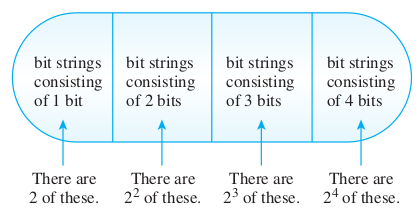
\includegraphics[scale=0.6]{../images/9.3.1.a.png}
\end{figure}

Applying the addition rule to the figure shows that there are \(2 + 2^2 + 2^3 + 2^4 = 30\) bit strings consisting of 
from one through four bits.
\end{proof}

\subsubsection{(b)}
How many bit strings consist of from five through eight digits?

\begin{proof}
By reasoning similar to that of part (a), there are \(2^5 + 2^6 + 2^7 + 2^8 = 480\) bit strings of from five through 
eight bits.
\end{proof}

\subsection{Exercise 2}
\subsubsection{(a)}
How many strings of hexadecimal digits consist of from one through three digits? (Recall that hexadecimal numbers are 
constructed using the 16 digits 0, 1, 2, 3, 4, 5, 6, 7, 8, 9, A, B, C, D, E, F.)

\begin{proof}
\(16^1 + 16^2 + 16^3 = 16 + 256 + 4096 = 4368\)
\end{proof}

\subsubsection{(b)}
How many strings of hexadecimal digits consist of from two through five digits?

\begin{proof}
\(16^2 + 16^3 + 16^4 + 16^5 = 256 + 4096 + 65536 + 1048576 = 1118464\)
\end{proof}

\subsection{Exercise 3}
\subsubsection{(a)}
How many integers from 1 through 999 do not have any repeated digits?

\begin{proof}
The set of integers from 1 through 999 with no repeated digit can be broken into three disjoint subsets: those from 
1 through 9, those from 1 through 99, and those from 100 through 999. Now constructing an integer from 100 through 
999 with no repeated digit can be thought of as a three-step process.

{\cy Step 1:} Choose a digit for the left-most position (where there are 9 choices because 0 cannot be chosen).

{\cy Step 2:} Choose a digit for the middle position (where there are also 9 choices because the digit in the left-most 
position cannot be reused but 0 can be used).

{\cy Step 3:} Choose a digit for the right-most position (where there are 8 choices because neither of the other two 
digits can be reused). 

Thus there are \(9 \cdot 9 \cdot 8\) integers from 100 through 999 with no repeated digit. Similar reasoning shows 
that there are \(9 \cdot 9\) integers from 10 through 99 with no repeated digit. Finally, there are clearly 9 
integers from 1 through 9 with no repeated digit. Hence, by the addition rule, the number of integers from 1 through 
999 with no repeated digit is \(9 + 9 \cdot 9 + 9 \cdot 9 \cdot 8 = 738\).
\end{proof}

\subsubsection{(b)}
How many integers from 1 through 999 have at least one repeated digit?

\begin{proof}
Let 

$x$ = number of integers from 1 through 999 with at least one repeated digit,

$y$ = total number of integers from 1 through 999,

$z$ = number of integers from 1 through 999 with no repeated digits.

Then \(x = y - z = 999 - 738 = 261\)
\end{proof}

\subsubsection{(c)}
What is the probability that an integer chosen at random from 1 through 999 has at least one repeated digit?

\begin{proof}
The probability that an integer chosen at random has at least one repeated digit is \(261/999 \approx 26.1\%\).
\end{proof}

\subsection{Exercise 4}
How many arrangements in a row of no more than three letters can be formed using the letters of the word NETWORK 
(with no repetitions allowed)?

\begin{proof}
Use the multiplication rule to count the elements in each of the three sets containing 1, 2, and 3 letters, 
respectively. Then, because these sets are disjoint, use the addition rule to compute the total number of elements 
in the three sets taken together.

\begin{figure}[ht!]
\centering
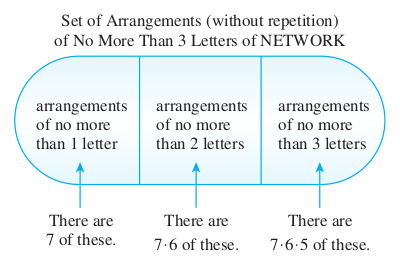
\includegraphics[scale=0.6]{../images/9.3.4.png}
\end{figure}

Applying the addition rule to the figure above shows that there are \(7 + 7 \cdot 6 + 7 \cdot 6 \cdot 5 = 259\) 
arrangements of three letters of the word NETWORK if repetition of letters is not permitted.
\end{proof}

\subsection{Exercise 5}
\subsubsection{(a)}
How many five-digit integers (integers from 10,000 through 99,999) are divisible by 5?

\begin{proof}
Let 

$x$ = number of integers from 10,000 through 99,999 that are divisible by 5,

$y$ = number of integers from 1 through 99,999 that are divisible by 5 = \(100,000 / 5 - 1 = 20,000 - 1 = 19,999\),

$z$ = number of integers from 1 through 9999 that are divisible by 5 = \(10,000 / 5 - 1 = 2000 - 1 = 1999\).

Then \(x = y - z = 19,999 - 1999 = 18,000\).
\end{proof}

\subsubsection{(b)}
What is the probability that a five-digit integer chosen at random is divisible by 5?

\begin{proof}
There are \(99,999 - 10,000 + 1 = 90,000\) five-digit integers. So: \(18,000 / 90,000 = 1/5 = 20\%\).
\end{proof}

\subsection{Exercise 6}
In a certain state, all license plates consist of from four to six symbols chosen from the 26 uppercase letters of the 
Roman alphabet together with the ten digits 0–9.

\subsubsection{(a)}
How many license plates are possible if repetition of symbols is allowed?

\begin{proof}
In this exercise the 26 letters in the alphabet plus the 10 digits give a total of 36 symbols that can be used on a 
license plate.

Imagine constructing a license plate with 4 symbols as a four-step process: {\cy step 1} is to fill in the first symbol, {\cy step 2} is to fill in the second symbol, {\cy step 3} is to fill in the third symbol, and {\cy step 4} is to fill in the fourth symbol. Because any one of the 36 symbols can be used in each step, by the multiplication rule, the number of license plates that use four symbols is \(36^4\). Similarly, the number that use 5 symbols is \(36^5\), and the number that use six symbols is \(36^6\). Thus because license plates can have anywhere from 4 to 6 symbols, the total number of plates with repeated symbols allowed is \(36^4 + 36^5 + 36^6 = 2,238,928,128\).
\end{proof}

\subsubsection{(b)}
How many license plates do not contain any repeated symbols?

\begin{proof}
When repetition is not allowed, the number of license plates that use four symbols is \(36 \cdot 35 \cdot 34 
\cdot 33\). The reason is that in the second step the symbol used in the first step cannot be used, so there are 
only 35 choices for the second step. In the third step, neither of the symbols used in the first two steps can be 
used, and so there are only 34 choices for the third step. And in the fourth step, none of the symbols used in the 
first three steps can be used, and so there are only 33 choices for the fourth step. Similarly, the number of 
license plates that use 5 symbols is \(36 \cdot 35 \cdot 34 \cdot 33 \cdot 32\), and the number that use six symbols is 
\(36 \cdot 35 \cdot 34 \cdot 33 \cdot 32 \cdot 31\). Thus the total number of license plates is \(36 \cdot 35 \cdot 
34 \cdot 33 + 36 \cdot 35 \cdot 34 \cdot 33 \cdot 32 + 36 \cdot 35 \cdot 34 \cdot 33 \cdot 32 \cdot 31 = 
1,449,063,000\).
\end{proof}

\subsubsection{(c)}
How many license plates have at least one repeated symbol?

\begin{proof}
Consider two sets: the set of plates with repetition not allowed and the set of plates that have a repeated symbol. 
Note that these two sets have no elements in common, and that since every license plate either has a repeated symbol 
or does not have a repeated symbol, every license plate considered in part (a) is in one of the two sets. In other 
words, the set of all license plates with repetition allowed is composed of two disjoint subsets: the set of 
plates with repetition not allowed and the set of plates that have a repeated symbol. Thus, by the difference rule, 
the number of license plates with a repeated symbol is the difference between the number of plates with repetition 
allowed minus the number of plates with repetition not allowed: \(2,238,928,128 - 1,449,063,000 = 789,865,128\).
\end{proof}

\subsubsection{(d)}
What is the probability that a license plate chosen at random has at least one repeated symbol?

\begin{proof}
The probability that a license plate chosen at random has at least one repeated symbol is 
\(789,865,128 / 2,238,928,128 \approx 35.3\%\).
\end{proof}

\subsection{Exercise 7}
At a certain company, passwords must be from 3–5 symbols long and composed from the 26 uppercase letters of the 
Roman alphabet, the ten digits 0–9, and the 14 symbols !, @, \#, \$, \%, \^\,, \&, *, (, ), -, +, \{, and \}.

\subsubsection{(a)}
How many passwords are possible if repetition of symbols is allowed?

\begin{proof}
The 26 letters in the alphabet plus the 10 digits plus the 14 special characters give a total of 50 symbols that can 
be used. By the multiplication rule, the number of passwords with 3, 4, and 5 symbols is \(50^3, 50^4\), and 
\(50^5\). Since the sets consisting of these passwords are disjoint, by the addition rule, the number of passwords is 

\(50^3 + 50^4 + 50^5 = 318,875,000\).
\end{proof}

\subsubsection{(b)}
How many passwords contain no repeated symbols?

\begin{proof}
There are \(50 \cdot 49 \cdot 48 = 117600\) passwords of length 3 with no repeated symbols.

There are \(50 \cdot 49 \cdot 48 \cdot 47 = 5527200\) passwords of length 4 with no repeated symbols.

There are \(50 \cdot 49 \cdot 48 \cdot 47 \cdot 46 = 254251200\) passwords of length 5 with no repeated symbols.

So by the addition rule, the total is \(254251200 + 5527200 + 117600 = 259,896,000\).
\end{proof}

\subsubsection{(c)}
How many passwords have at least one repeated symbol?

\begin{proof}
\(318,875,000 - 259,896,000 = 58,979,000\)
\end{proof}

\subsubsection{(d)}
What is the probability that a password chosen at random has at least one repeated symbol?

\begin{proof}
\(58,979,000 / 318,875,000 \approx 18.5\% \)
\end{proof}

\subsection{Exercise 8}
In a certain country license plates consist of zero or one digit followed by four or five uppercase letters from the 
Roman alphabet.

\subsubsection{(a)}
How many different license plates can the country produce?

{\it Hint:} One approach is to divide the license plates into four groups depending on the number of digits and 
letters they contain. Another approach is to consider creating a license plate as a two-step process: step 1: 
either choose one digit or do not choose a digit; and step 2: choose 4 or 5 letters.

\begin{proof}
There are four groups: 1. No digit, 4 letters, 2. One digit, 4 letters, 3. No digit, 5 letters, 4. One digit, 5 
letters.

First group has \(26^4\) possibilities. Second group has \(10 \cdot 26^4\) possibilities.

Third group has \(26^5\) possibilities. Fourth group has \(10 \cdot 26^5\) possibilities.

In total: \(26^4 + 10 \cdot 26^4 + 26^5 + 10 \cdot 26^5 = 11(26^4 + 26^5) = 11 \cdot 26^4 (1 + 26) = 11 \cdot 26^4 
\cdot 27 = 135,721,872\)
\end{proof}

\subsubsection{(b)}
How many license plates have no repeated letter?

\begin{proof}
Choosing 4 non-repeated letters, no digit: \(26 \cdot 25 \cdot 24 \cdot 23 = 358,800\), with one digit: \(10 \cdot 
358,800 = 3,588,000\)

Choosing 5 non-repeated letters, no digit: \(26 \cdot 25 \cdot 24 \cdot 23 \cdot 22 = 7,893,600\), with one digit:
\(10 \cdot 7,893,600 = 78,936,000\)

Total: \(358,800 + 3,588,000 + 7,893,600 + 78,936,000 = 90,776,400\)
\end{proof}

\subsubsection{(c)}
How many license plates have at least one repeated letter?

\begin{proof}
\(135,721,872 - 90,776,400 = 44,945,472\)
\end{proof}

\subsubsection{(d)}
What is the probability that a license plate has a repeated letter?

\begin{proof}
\(44,945,472 / 135,721,872 \approx 33.11\%\)
\end{proof}

\subsection{Exercise 9}
\subsubsection{(a)}
Consider the following algorithm segment:

\begin{tabbing}
{\bf for} \= \(i \coloneqq 1\) {\bf to} 4 \\
          \> {\bf for} \= \(j \coloneqq 1\) {\bf to} $i$ \\
          \>           \> {\it [Statements in body of inner loop.]} \\
          \>           \> {\it [None contain branching statements that lead outside the loop.]} \\
          \> {\bf next} $j$ \\
{\bf next} $i$
\end{tabbing}

How many times will the inner loop be iterated when the algorithm is implemented and run?

\begin{proof}
Each column of the table below corresponds to a pair of values of $i$ and $j$ for which the inner loop will be 
iterated.

\begin{figure}[ht!]
\centering
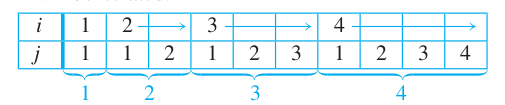
\includegraphics[scale=0.6]{../images/9.3.9.a.png}
\end{figure}

Since there are \(1 + 2 + 3 + 4 = 10\) columns, the inner loop will be iterated ten times.
\end{proof}

\subsubsection{(b)}
Let $n$ be a positive integer, and consider the following algorithm segment:

\begin{tabbing}
{\bf for} \= \(i \coloneqq 1\) {\bf to} $n$ \\
          \> {\bf for} \= \(j \coloneqq 1\) {\bf to} $i$ \\
          \>           \> {\it [Statements in body of inner loop.]} \\
          \>           \> {\it [None contain branching statements that lead outside the loop.]} \\
          \> {\bf next} $j$ \\
{\bf next} $i$
\end{tabbing}

How many times will the inner loop be iterated when the algorithm is implemented and run?

\begin{proof}
\(1 + 2 + \cdots + n = n(n+1)/2\)
\end{proof}

\subsection{Exercise 10}
A calculator has an eight-digit display and a decimal point that is located at the extreme right of the number 
displayed, or at the extreme left, or between any pair of digits. The calculator can also display a minus sign at the 
extreme left of the number. How many distinct numbers can the calculator display? (Note that certain numbers are 
equal, such as 1.9, 1.90, and 01.900, and should, therefore, not be counted twice.)

\begin{proof}
Let's solve this problem for a 1-digit display, then 2-digit, and so on. Also, let's first solve the problem only
for nonnegative numbers.

{\bf 1-digit display:} First let's consider nonnegative numbers. A number $x$ can be in the range \(0 \leq x < 1\)
(if the decimal point is on the left) or in the range \(1 \leq x < 10\) (if the decimal point is on the right).

For the first range there are 10 possibilities: \(.0, .1, .2, .3, .4, .5, .6, .7, .8, .9\);

for the second range we cannot allow the digit to be 0, otherwise \(x < 1\), so there are only 9 possibilities: 
\(1., 2., 3., 4., 5., 6., 7., 8., 9.\);

so we have \(10^1 + (10^1 - 1) = 19\) nonnegative numbers.

{\bf 2-digit display:} First let's consider nonnegative numbers. A number $x$ can be in the range \(0 \leq x < 1\)
(if the decimal point is on the left) or in the range \(1 \leq x < 10\) (if the decimal point is in the middle) or in 
the range \(10 \leq x < 100\) (if the decimal point is on the right).

For the first range there are \(10^2\) possibilities: \(.00, .01, \ldots, .09, .10, .11, \ldots, .99\); 

for the second range we cannot allow the left-most digit to be 0, otherwise \(x < 1\), so there are only 90 
possibilities: \(1.0, 1.1, 1.2, \ldots, 9.9\);

for the third range there are also 90 possibilities: \(10., 11., 12., \ldots, 99.\) because, similarly, the first digit 
cannot be zero; so we have \(10^2 + 10^1 \cdot (10^1 - 1) + 10^1 \cdot (10^1 - 1) = 100 + 90 + 90 = 280\) nonnegative 
numbers.

{\bf 3-digit display:} A number $x$ can be in one of the ranges \(0 \leq x < 1\) or \(1 \leq x < 10\) or \(10 \leq x 
< 100\) or \(100 \leq x < 1000\).

Similar to the above, we have \(10^3 + 10^2 \cdot (10^1 - 1) + 10^2 \cdot (10^1 - 1) + 10^2 \cdot (10^1 - 1) = 
1000 + 900 + 900 + 900 = 3700\) nonnegative numbers.

So the general formula for $n$ digits is: \(10^n + n \cdot 10^{n-1} \cdot 9\). For an $n=8$-digit display, there are
\(10^8 + 8 \cdot 10^7 \cdot 9 = 100,000,000 + 10,000,000 \cdot 72 = 820,000,000\) unique nonnegative numbers.

{\bf Conclusion:} 820,000,000 nonnegative and 820,000,000 nonpositive numbers (obtained by putting the negative sign
in front of them) gives 1,640,000,000 numbers. However 0 and \(-0\) are the same, so it's 1,639,999,999 numbers.
\end{proof}

\subsection{Exercise 11}
\subsubsection{(a)}
How many ways can the letters of the word QUICK be arranged in a row?

\begin{proof}
The answer is the number of permutations of the five letters in QUICK, which equals \(5! = 120\).
\end{proof}

\subsubsection{(b)}
How many ways can the letters of the word QUICK be arranged in a row if the Q and the U must remain next to each other 
in the order QU?

\begin{proof}
Because \boxed{QU} (in order) is to be considered as a single unit, the answer is the number of permutations of 
the four symbols \boxed{QU}, I, C, K. This is \(4! = 24\).
\end{proof}

\subsubsection{(c)}
How many ways can the letters of the word QUICK be arranged in a row if the letters QU must remain together but may be 
in either the order QU or the order UQ?

\begin{proof}
By part (b), there are 4! arrangements of \boxed{QU}, I, C, K. Similarly, there are 4! arrangements of \boxed{QU}, I, 
C, K. Therefore, by the addition rule, there are \(4! + 4! = 48\) arrangements in all.
\end{proof}

\subsection{Exercise 12}
\subsubsection{(a)}
How many ways can the letters of the word THEORY be arranged in a row?

\begin{proof}
\(6! = 720\)
\end{proof}

\subsubsection{(b)}
How many ways can the letters of the word THEORY be arranged in a row if T and H must remain next to each other 
as either TH or HT?

\begin{proof}
\(5! + 5! = 240\)
\end{proof}

\subsection{Exercise 13}
A group of eight people are attending the movies together.

\subsubsection{(a)}
Two of the eight insist on sitting side-by-side. In how many ways can the eight be seated together in a row?

\begin{proof}
Let

$x$ = the number of ways to place eight people in a row keeping $A$ and $B$ together,

$y$ = the number of ways to arrange \boxed{AB}, C, D, E, F, G, H,

$z$ = the number of ways to arrange \boxed{BA}, C, D, E, F, G, H.

Then \(x = y+z = 7!+7! = 5040+5040 = 10080\).
\end{proof}

\subsubsection{(b)}
Two of the people do not like each other and do not want to sit side-by-side. Now how many ways can the eight be seated 
together in a row?

\begin{proof}
Let

$x$ = the number of ways to place eight people in a row keeping $A$ and $B$ apart,

$y$ = the number of ways to place eight people in a row,

$z$ = the number of ways to place eight people in a row keeping $A$ and $B$ together.

By part (a) $z = 10080$. So \(x = y-z = 8!-10080 = 40320-10080 = 30240\).
\end{proof}

\subsection{Exercise 14}
An early compiler recognized variable names according to the following rules: Numeric variable names had to begin 
with a letter, and then the letter could be followed by another letter or a digit or by nothing at all. String 
variable names had to begin with the symbol \$ followed by a letter, which could then be followed by another letter or 
a digit or by nothing at all. How many distinct variable names were recognized by this compiler?

\begin{proof}
the number of variable names = the number of numeric variable names + the number of string variable names = 
\((26 + 26 \cdot 36) + (26 + 26 \cdot 36) = 1924\).
\end{proof}

\subsection{Exercise 15}
Identifiers in a certain database language must begin with a letter, and then the letter may be followed by other 
characters, which can be letters, digits, or underscores (\_). However, 82 keywords (all consisting of 15 or fewer 
characters) are reserved and cannot be used as identifiers. How many identifiers with 30 or fewer characters are 
possible? (Write the answer using summation notation and evaluate it using a formula from Section 5.2.)

\begin{proof}
For the first character there are 26 choices (letters).

For other characters there are 37 choices (letters, digits, or underscore).

So, there are \(26\) length 1 identifiers, \(26 \cdot 37\) length-2 identifiers, ..., and \(26 \cdot 37^{29}\) 
length-3 identifiers. So the number of identifiers with 30 or fewer characters is:
\[
26+26 \cdot 37 + \cdots + 26 \cdot 37^{29} = 26(1+37+37^2+\cdots+37^{29}) = 26 \cdot \frac{37^{30}-1}{37-1}
\]
\end{proof}

\subsection{Exercise 16}
\subsubsection{(a)}
If any seven digits could be used to form a telephone number, how many seven-digit telephone numbers would not 
have any repeated digits?

\begin{proof}
\(10 \cdot 9 \cdot 8 \cdot 7 \cdot 6 \cdot 5 \cdot 4 = 604,800\)
\end{proof}

\subsubsection{(b)}
How many seven-digit telephone numbers would have at least one repeated digit?

\begin{proof}
Let $x$ = the number of phone numbers with at least one repeated digit,

$y$ = the total number of phone numbers,

$z$ = the number of phone numbers with no repeated digits,

then \(x = y - z = 10^7 - 604,800 = 9,395,200\).
\end{proof}

\subsubsection{(c)}
What is the probability that a randomly chosen seven-digit telephone number would have at least one repeated digit?

\begin{proof}
\(9,395,200 / 10,000,000 \approx 93.95\%\)
\end{proof}

\subsection{Exercise 17}
\subsubsection{(a)}
How many strings of four hexadecimal digits do not have any repeated digits?

\begin{proof}
\(16 \cdot 15 \cdot 14 \cdot 13 = 43680\)
\end{proof}

\subsubsection{(b)}
How many strings of four hexadecimal digits have at least one repeated digit?

\begin{proof}
\(16^4 - 43680 = 65536 - 43680 = 21856\)
\end{proof}

\subsubsection{(c)}
What is the probability that a randomly chosen string of four hexadecimal digits has at least one repeated digit?

\begin{proof}
\(21856 / 65536 \approx 33.34\)
\end{proof}

\subsection{Exercise 18}
Just as the difference rule gives rise to a formula for the probability of the complement of an event, so the addition 
and inclusion/exclusion rules give rise to formulas for the probability of the union of mutually disjoint events and 
for a general union of (not necessarily mutually exclusive) events.

\subsubsection{(a)}
Prove that for mutually disjoint events $A$ and $B$, \(P(A \cup B) = P(A) + P(B)\).

\begin{proof}
Let $A$ and $B$ be mutually disjoint events in a sample space $S$. By the addition rule, \(N(A \cup B) = N(A) + 
N(B)\). Therefore, by the equally likely probability formula,
\[
P(A \cup B)=\frac{N(A\cup B)}{N(S)}=\frac{N(A)+N(B)}{N(S)}= \frac{N(A)}{N(S)} + \frac{N(B)}{N(S)} = P(A) + P(B).
\]
\end{proof}

\subsubsection{(b)}
Prove that for any events $A$ and $B$, \(P(A \cup B) = P(A) + P(B) - P(A \cap B)\).

\begin{proof}
Let $A$ and $B$ be any events in a sample space $S$. By the inclusion / exclusion rule, \(N(A \cup B) = N(A) + N(B) -
N(A \cap B)\). Therefore, by the equally likely probability formula,
\[
P(A \cup B) = \frac{N(A \cup B)}{N(S)}=\frac{N(A) + N(B) - N(A \cap B)}{N(S)}= \frac{N(A)}{N(S)} + \frac{N(B)}{N(S)} -
\frac{N(A \cap B)}{N(S)}
\]
\(= P(A) + P(B) - P(A \cap B)\).
\end{proof}

\subsection{Exercise 19}
A combination lock requires three selections of numbers, each from 1 through 39. Suppose the lock is constructed in 
such a way that no number may be used twice in a row but the same number may occur both first and third. For 
example, 20 13 20 would be acceptable, but 20 20 13 would not. How many different combinations are possible?

\begin{proof}
There are 39 choices for the first selection. Then 38 choices for the second selection. Now there are 38 choices
for the third selection: it cannot be the same as the second selection, but it can be the same as the first. So 
by the multiplication rule \(39 \cdot 38 \cdot 38\) possible combinations.
\end{proof}

\subsection{Exercise 20}
\subsubsection{(a)}
How many integers from 1 through 100,000 contain the digit 6 exactly once?

\begin{proof}
Use strings of five digits to represent integers from 1 to 100,000 that contain the digit 6 exactly once. For example, 
use 00306 to represent 306. Strings of six digits are not needed because 100,000 does not contain a 6. Imagine 
constructing a five-digit string that contains exactly one 6 as a five-step operation to fill in five positions with 
five digits: \(\underset{1}{\fbl} \underset{2}{\fbl} \underset{3}{\fbl} \underset{4}{\fbl} \underset{5}{\fbl}\).

{\cy Step 1:} Choose one of the five positions for the 6.

{\cy Step 2:} Choose a digit for the left-most remaining position.

{\cy Step 3:} Choose a digit for the next remaining position to the right.

{\cy Step 4:} Choose a digit for the next remaining position to the right.

{\cy Step 5:} Choose a digit for the right-most position.

Since there are 5 choices for step 1 (any one of the five positions) and 9 choices for each of steps 2–5 (any digit 
except 6), by the multiplication rule, the number of ways to perform this operation is \(5 \cdot 9 \cdot 9 \cdot 9 
\cdot 9 = 32,805\). Hence there are 32,805 integers from 1 to 100,000 that contain the digit 6 exactly once.
\end{proof}

\subsubsection{(b)}
How many integers from 1 through 100,000 contain the digit 6 at least once?

\begin{proof}
Let $x$ = the number of integers from 1 through 100,000,

$y$ = the number of integers from 1 through 100,000, that do not contain the digit 6,

$z$ = the number of integers from 1 through 100,000, that contain the digit 6 at least once.

Then \(z = x - y = 100,000 - (9^5 + 1) = 40950\).
\end{proof}

\subsubsection{(c)}
If an integer is chosen at random from 1 through 100,000, what is the probability that it contains two or more occurrences of the digit 6?

\begin{proof}
Let $x$ = the number of integers from 1 through 100,000, that contain the digit 6 at least once,

$y$ = the number of integers from 1 through 100,000, that contain the digit 6 exactly once,

$z$ = the number of integers from 1 through 100,000, that contain the digit 6 two or more times.

Then \(z = x - y = 40950 - 32805 = 8145\). Then the probability is \(8145/100000 = 8.145\%\)
\end{proof}

\subsection{Exercise 21}
Six new employees, two of whom are married to each other, are to be assigned six desks that are lined up in a row. If 
the assignment of employees to desks is made randomly, what is the probability that the married couple will have 
nonadjacent desks? (Hint: The event that the couple have nonadjacent desks is the complement of the event that they 
have adjacent desks.)

\begin{proof}
There are \(6! = 720\) possible assignments. The number of assignments where the married couple are adjacent is 
\(2 \cdot 5! = 240\) since we can think of the adjacent married couple as one, and with the remaining 4 employees, 
there are 5 people to assign desks, but we can also switch the married couple's positions. So \(720-240 = 480\) 
assignments have the married couple in nonadjacent desks. The probability is \(480/720 = 2/3\).
\end{proof}

\subsection{Exercise 22}
\subsubsection{(a)}
Consider strings of length $n$ over the set \(\{a, b, c, d\}\). How many such strings contain at least one pair of 
adjacent characters that are the same?

\begin{proof}
Let $x$ = the total number of all strings = \(4^n\), 

$y$ = the number of strings that have no pairs of adjacent 
characters that are the same = \(4 \cdot \underbrace{3 \cdot \cdots \cdot 3}_{n-1 \text{ times}} = 4 \cdot 3^{n-1}\),

$z$ = the number of strings contain at least one pair of 
adjacent characters that are the same = \(x - y = 4^n - 4 
\cdot 3^{n-1}\).
\end{proof}

\subsubsection{(b)}
If a string of length ten over \(\{a, b, c, d\}\) is chosen at random, what is the probability that it contains at 
least one pair of adjacent characters that are the same?

\begin{proof}
When $n=10$, the number of all strings is \(4^{10} = 1048576\) and the number of strings that contain at least 
one pair of adjacent characters that are the same is \(4^{10} - 4 \cdot 3^9 = 1048576 - 4 \cdot 19683 = 969844\)
so the probability is \(969844 / 1048576 \approx 92.49\%\).
\end{proof}

\subsection{Exercise 23}
\subsubsection{(a)}
How many integers from 1 through 1,000 are multiples of 4 or multiples of 7?

\begin{proof}
Let $A$ = the set of integers that are multiples of 4 and $B$ = the set of integers that are multiples of 7. Then 
\(A \cap B\) = the set of integers that are multiples of 28. 

Now \(N(A) = 250\) because

\begin{center}
\begin{tabular}{ccccccccccc}
1&2&3&4&5&6&7&8& \(\ldots\) &999&1000 \\
&&&\(\updownarrow\)&&&&\(\updownarrow\)&&&\(\updownarrow\) \\
&&&\(4 \cdot 1\)&&&&\(4 \cdot 2\)& \(\ldots\) &&\(4 \cdot 250\) \\
\end{tabular}
\end{center}

or equivalently, because \(1000 = 4 \cdot 250\). Also \(N(B) = 142\) because

\begin{center}
\begin{tabular}{cccccccccccccc}
1&2&3&4&5&6&7& \(\ldots\) &14& \(\ldots\) &994&995& \(\ldots\) &1000 \\
&&&&&&\(\updownarrow\)&&\(\updownarrow\)&&\(\updownarrow\)&& \\
&&&&&&\(7 \cdot 1\)&&\(7 \cdot 2\)&&\(7 \cdot 142\)&& \\
\end{tabular}
\end{center}

or equivalently because \(1000 = 7 \cdot 142 + 6\). And \(N(A \cap B) = 35\) because

\begin{center}
\begin{tabular}{ccccccccccc}
1&2&3& \(\ldots\) &28& \(\ldots\) &56& \(\ldots\) &980& \(\ldots\) &1000 \\
&&&&\(\updownarrow\)&&\(\updownarrow\)&&\(\updownarrow\)&& \\
&&&&\(28 \cdot 1\)&&\(28 \cdot 2\)&&\(28 \cdot 35\)&& \\
\end{tabular}
\end{center}

or equivalently because \(1000 = 28 \cdot 35 + 20\). So \(N(A \cup B) = 250 + 142 - 35 = 357\).
\end{proof}

\subsubsection{(b)}
Suppose an integer from 1 through 1,000 is chosen at random. Use the result of part (a) to find the probability that the integer is a multiple of 4 or a multiple of 7.

\begin{proof}
\(357/1000 = 35.7\%\)
\end{proof}

\subsubsection{(c)}
How many integers from 1 through 1,000 are neither multiples of 4 nor multiples of 7?

\begin{proof}
\(1000-357 = 643\)
\end{proof}

\subsection{Exercise 24}
\subsubsection{(a)}
How many integers from 1 through 1,000 are multiples of 2 or multiples of 9?

\begin{proof}
\(\floor{1000 / 2} = 500\) multiples of 2, \(\floor{1000 / 9} = 111\) multiples of 9, and \(\floor{1000 / 18} = 55\)
multiples of 18 (which are double-counted). So: \(500 + 111 - 55 = 556\).
\end{proof}

\subsubsection{(b)}
Suppose an integer from 1 through 1,000 is chosen at random. Use the result of part (a) to find the probability that the integer is a multiple of 2 or a multiple of 9.

\begin{proof}
\(556/1000=55.6\%\)
\end{proof}

\subsubsection{(c)}
How many integers from 1 through 1,000 are neither multiples of 2 nor multiples of 9?

\begin{proof}
\(1000-556=444\)
\end{proof}

\subsection{Exercise 25}
{\it Counting Strings:}

\subsubsection{(a)}
Make a list of all bit strings of lengths 0, 1, 2, 3, and 4 that do not contain the bit pattern 111.

\begin{proof}
\(\lambda\), 0, 1, 00, 01, 10, 11, 000, 001, 010, 100, 011, 101, 110, 0000, 0001, 0010, 0011, 0100, 0101, 0110, 1000, 1001, 1010, 1011, 1100, 1101
\end{proof}

\subsubsection{(b)}
For each integer \(n \geq 0\), let \(d_n =\) the number of bit strings of length $n$ that do not contain the bit 
pattern 111. Find \(d_0, d_1, d_2, d_3\), and \(d_4\).

\begin{proof}
\(d_0 = 1, d_1 = 2, d_2 = 4, d_3 = 7, d_4 = 13\)
\end{proof}

\subsubsection{(c)}
Find a recurrence relation for \(d_0, d_1, d_2, \ldots\).

\begin{proof}
Let $k$ be an integer with \(k \geq 3\). Any string of length $k$ that does not contain the bit pattern 111 starts 
either with a 0 or with a 1. If it starts with a 0, this can be followed by any string of \(k - 1\) bits that does 
not contain the pattern 111. There are \(d_{k-1}\) of these. If the string starts with a 1, then the first two 
bits are 10 or 11. If the first two bits are 10, then these can be followed by any string of \(k - 2\) bits that does 
not contain the pattern 111. There are \(d_{k-2}\) of these. If the string starts with a 11, then the third bit 
must be 0 (because the string does not contain 111), and these three bits can be followed by any string of \(k - 3\) 
bits that does not contain the pattern 111. There are \(d_{k-3}\) of these. Therefore, for every integer 
\(k \geq 3, d_k = d_{k-1} + d_{k-2} + d_{k-3}\).
\end{proof}

\subsubsection{(d)}
Use the results of parts (b) and (c) to find the number of bit strings of length 5 that do not contain the pattern 
111.

\begin{proof}
\(d_5 = d_4 + d_3 + d_2 = 13+7+4 = 24\)
\end{proof}

\subsection{Exercise 26}
{\it Counting Strings:} Consider the set of all strings of
$a$’s, $b$’s, and $c$’s.

\subsubsection{(a)}
Make a list of all of these strings of lengths 0, 1, 2, and 3 that do not contain the pattern $aa$.

\begin{proof}
Length 0: \(\lambda\), Length 1: \(a, b, c\), Length 2: \(\Ccancel{aa}, ab, ac, ba, bb, bc, ca, cb, cc\),

Length 3: \(\Ccancel{aaa}, \Ccancel{aab}, \Ccancel{aac}, aba, abb, abc, aca, acb, acc\), 
\(\Ccancel{baa}, bab, bac, bba, bbb, bbc, bca, bcb, bcc\), 
\(\Ccancel{caa}, cab, cac, cba, cbb, cbc, cca, ccb, ccc\).
\end{proof}

\subsubsection{(b)}
For each integer \(n \geq 0\), let \(s_n =\) the number of strings of $a$’s, $b$’s, and $c$’s of length $n$ that do 
not contain the pattern $aa$. Find \(s_0, s_1, s_2\), and \(s_3\).

\begin{proof}
\(s_0 = 1, s_1 = 3, s_2 = 8, s_3 = 22\)
\end{proof}

\subsubsection{(c)}
Find a recurrence relation for \(s_0, s_1, s_2, \ldots\).

\begin{proof}
Let $s$ be a string of length $k$ that does not contain the pattern $aa$. 

If $x$ starts with $b$ or $c$ then it can be followed by any string of length $k-1$ that does not contain the 
pattern $aa$. There are \(s_{k-1}\) of those, so there are \(2s_{k-1}\) such strings which $x$ can be: \(s_{k-1}\) of 
them starting with $b$ and \(s_{k-1}\) of them starting with $c$.

If $x$ starts with $a$ then it can be followed by a $b$ or a $c$ and then a string of length $k-2$ that does not 
contain the pattern $aa$. There are \(s_{k-2}\) of those, so there are \(2s_{k-2}\) such strings that $x$ can be: 
\(s_{k-2}\) of them starting with $ab$ and \(s_{k-2}\) of them starting with $ac$.

So \(s_k = 2s_{k-1} + 2s_{k-2}\).
\end{proof}

\subsubsection{(d)}
Use the results of parts (b) and (c) to find the number of strings of $a$’s, $b$’s, and $c$’s of length four that do 
not contain the pattern $aa$.

\begin{proof}
\(s_4 = 2s_3 + 2s_2 = 2(22+8) = 60\).
\end{proof}

\subsubsection{(e)}
Use the technique described in Section 5.8 to find an explicit formula for \(s_0, s_1, s_2, \ldots\).

\begin{proof}
\(s_k = 2s_{k-1} + 2s_{k-2}\) so the characteristic equation is \(t^2 - 2t-2 = 0\) which has the solutions
\[
\frac{2 \pm \sqrt{(-2)^2 - 4(1)(-2)}}{2} = \frac{2 \pm \sqrt{4+8}}{2} = \frac{2 \pm 2\sqrt{3}}{2} = 1 \pm \sqrt{3}
\]
The general solution has the form \(s_k = A(1+\sqrt{3})^k + B(1-\sqrt{3})^k\). When $k=0$ we have
\[
s_0 = 1 = A(1+\sqrt{3})^0 + B(1-\sqrt{3})^0 = A+B
\]
which gives $B = 1-A$; and when $k=1$ we have 
\[
s_1 = 3 = A(1+\sqrt{3})^1 + B(1-\sqrt{3})^1 = A+B + \sqrt{3}(A-B)
\]
so we get \(3 = 1 + \sqrt{3}(A - (1-A)) = 1+\sqrt{3}(2A-1)\), solving we get \(\frac{2}{\sqrt{3}} = 2A-1\) so 
\(\frac{1}{\sqrt{3}} + \frac{1}{2} = A\). Then \(B = \frac{1}{2} - \frac{1}{\sqrt{3}}\). So
\[
s_n = \left(\frac{1}{2} + \frac{1}{\sqrt{3}}\right)(1+\sqrt{3})^n + \left(\frac{1}{2} - \frac{1}{\sqrt{3}}\right)
(1-\sqrt{3})^n
\]
\end{proof}

\subsection{Exercise 27}
For each integer \(n \geq 0\), let \(a_k\) be the number of bit strings of length $n$ that do not contain the pattern 
101.

\subsubsection{(a)}
Show that \(a_k = a_{k-1} + a_{k-3} + a_{k-4} + \cdots + a_0 + 2\), for every integer \(k \geq 3\).

\begin{proof}
Assume \(k \geq 3\) and $s$ is a string of length $k$ that does not contain the pattern 101.

If $s$ begins with a 0 then it can be followed by a string of length $k-1$ that does not contain the pattern 101.
There are \(a_{k-1}\) of these.

If $s$ begins with a 1 then consider the following. If it begins with:

100 then it can be followed by a string of length $k-3$ that does not contain the pattern 101, and there are 
\(a_{k-3}\) of them,

1100 then it can be followed by a string of length $k-4$ that does not contain the pattern 101, and there are 
\(a_{k-4}\) of them,

11100 then it can be followed by a string of length $k-5$ that does not contain the pattern 101, and there are 
\(a_{k-5}\) of them,

\(\underbrace{11\ldots 1}_{k-3}00\), then it can be followed by a string of length $k-(k-1) = 1$ that does not 
contain the pattern 101, and there are \(a_1\) of them,

\(\underbrace{11\ldots 1}_{k-2}00\), then it can be followed by a string of length $k-k = 0$ that does not 
contain the pattern 101, and there are \(a_0\) of them,

\(\underbrace{11\ldots 1}_{k-1}\), then it can be followed by 1 or 0, and there are \(2\) of them.

So \(a_k= a_{k-1} + a_{k-3} + a_{k-4} + \cdots + a_0 + 2\).
\end{proof}

\subsubsection{(b)}
Use the result of part (a) to show that if \(k \geq 3\), then \(a_k = 2a_{k-1} - a_{k-2} + a_{k-3}\).

\begin{proof}
By part (a) we have \(a_{k-1} = a_{k-2} + a_{k-4} + a_{k-5} + \cdots + a_0 + 2\).

So \(a_{k-1} + a_{k-3} = a_{k-2} + a_{k-3} + a_{k-4} + a_{k-5} + \cdots + a_0 + 2\).

So \(a_{k-1} - a_{k-2} + a_{k-3} = a_{k-3} + a_{k-4} + a_{k-5} + \cdots + a_0 + 2\).

So \(2a_{k-1} - a_{k-2} + a_{k-3} = a_{k-1} + a_{k-3} + a_{k-4} + a_{k-5} + \cdots + a_0 + 2\).

Notice the right-hand side is equal to \(a_k\) by part (a).
\end{proof}

\subsection{Exercise 28}
For each integer \(n \geq 2\) let \(a_n\) be the number of permutations of \(\{1, 2, 3, \ldots, n\}\) in which no 
number is more than one place removed from its “natural” position. Thus \(a_1 = 1\) since the one permutation of 
\(\{1\}\), namely, 1, does not move 1 from its natural position. Also, \(a_2 = 2\) since neither of the two 
permutations of \(\{1, 2\}\), namely, 12 and 21, moves either number more than one place from its natural position.

\subsubsection{(a)}
Find \(a_3\).

\begin{proof}
\(a_3 = 3\) (The three permutations that do not move more than one place from their “natural” positions are 213, 132, 
and 123.)
\end{proof}

\subsubsection{(b)}
Find a recurrence relation for \(a_1, a_2, a_3, \ldots\).

\begin{proof}
Let's try to see a relationship between \(a_2 = 2\) and \(a_3 = 3\). We need to add the new element 3. Since we 
cannot move 3 more than one from its natural position, it can be in position 2 or 3. If it's in position 3, like 
\_\_3, then both of the permutations from \(a_2\) work: 123, 213. If it's in position 2, then 2 must be in position 
3: \_23, so there is only one possibility left: 123.

Let's find $a_4$. There are \(4! = 24\) permutations of \(\{1,2,3,4\}\), but there are only 5 which do not move more
more than one place: 1234, 2134, 1243, 2143, 1324. So \(a_4 = 5\). 

But how is it obtained from \(a_3\)? There are 3 permutations in $a_3$: 123, 132, 213. Now we need to add 
the element 4 to them. 4 can be either in position 3 or position 4. If it's in position 4, like \_\_\_4, then all 
the permutations from $a_3$ work: 1234, 2134, 1324. If 4 is in position 3, then 3 must be in position 4: \_\_43, so now
there are $a_2$ ways to fill the two spots: 1243, 2143.

So we can see that the general form of the recurrence is: \(a_n = a_{n-1} + a_{n-2}\).
\end{proof}

\subsection{Exercise 29}
Refer to Example 9.3.5.

\subsubsection{(a)}
Write the following IP address in dotted decimal form: 11001010 00111000 01101011 11101110

\begin{proof}
\(11001010_2 = 2 + 23 + 26 + 27 = 202\)

\(00111000_2 = 23 + 24 + 25 = 56\)

\(01101011_2 = 1 + 2 + 23 + 25 + 26 = 107\)

\(11101110_2 = 2 + 22 + 23 + 25 + 26 + 27 = 238\)

So the answer is 202.56.107.238.
\end{proof}

\subsubsection{(b)}
How many Class A networks can there be?

\begin{proof}
The network ID for a Class A network consists of 8 bits and begins with 0. If all possible combinations of eight 0’s 
and 1’s that start with a 0 were allowed, there would be 2 choices (0 or 1) for each of the 7 positions from the 
second through the eighth. This would give \(2^7 = 128\) possible ID’s. But because neither 00000000 nor 01111111 is 
allowed, the total is reduced by 2, so there are 126 possible Class A networks.
\end{proof}

\subsubsection{(c)}
What is the dotted decimal form of the IP address for a computer in a Class A network?

\begin{proof}
Let \(w.x.y.z\) be the dotted decimal form of the IP address for a computer in a Class A network. Because the 
network IDs for a Class A network go from 00000001 (= 1) through 01111110 (= 126), $w$ can be any integer from 1 
through 126. In addition, each of \(x, y\), and \(z\) can be any integer from 0 (= 00000000) through 255 (= 
11111111), except that \(x, y\), and \(z\) cannot all be 0 simultaneously and cannot all be 255 simultaneously.
\end{proof}

\subsubsection{(d)}
How many host IDs can there be for a Class A network?

\begin{proof}
Twenty-four positions are allocated for the host ID in a Class A network. If each could be either 0 or 1, there 
would be \(2^{24} = 16,777,216\) possible host IDs. But neither all 0’s nor all 1’s is allowed, which reduces the 
total by 2. Thus there are 16,777,214 possible host IDs in a Class A network.
\end{proof}

\subsubsection{(e)}
How many Class C networks can there be?

\begin{proof}
The network ID for a Class C network consists of 24 bits and begins with 110. There are 2 choices (0 or 1) for each 
of the 21 positions from the fourth through the twenty-fourth. This gives \(2^{21}\) possible ID’s. 
\end{proof}

\subsubsection{(f)}
What is the dotted decimal form of the IP address for a computer in a Class C network?

\begin{proof}
Let \(w.x.y.z\) be the dotted decimal form of the IP address for a computer in a Class C network. The 
network IDs for a Class C network go from 110000000000000000000000 through 110111111111111111111111.

If we break these down into chunks of 8 bits and convert them to binary, we get:

\(11000000_2 = 192_{10}, 00000000_2 = 0_{10}, 00000000_2 = 0_{10}\),

\(11011111_2 = 223_{10}, 11111111_2 = 255_{10}, 11111111_2 = 255_{10}\).

As dotted decimals they range from 192.0 to 223.255. So \(192 \leq w \leq 223\), \(0 \leq x \leq 255\), 
\(0 \leq y \leq 255\), \(0 \leq z \leq 255\).
\end{proof}

\subsubsection{(g)}
How many host IDs can there be for a Class C network?

\begin{proof}
There are only 8 bits for host IDs in a Class C network, but a host ID may not consist of either all 0’s or all 1’s. 
Therefore \(2^8 - 2 = 254\) host IDs.
\end{proof}

\subsubsection{(h)}
How can you tell, by looking at the first of the four numbers in the dotted decimal form of an IP address, what 
kind of network the address is from? Explain.

\begin{proof}
For Class A networks \(0 \leq w \leq 126\), for Class B networks \(128 \leq w \leq 191\), for Class C networks 
\(192 \leq w \leq 223\). So we can tell from this info what kind of network an address is from.
\end{proof}

\subsubsection{(i)}
An IP address is 140.192.32.136. What class of network does it come from?

\begin{proof}
Observe that \(140 = 128 + 8 + 4 = 10001100_2\), which begins with 10. Thus the IP address comes from a Class B 
network. An alternative solution uses the result of Example 9.3.5: Network IDs for Class B networks range from 128 
through 191. Thus, since \(128 \leq 140 \leq 191\), the given IP address is from a Class B network.
\end{proof}

\subsubsection{(j)}
An IP address is 202.56.107.238. What class of network does it come from?

\begin{proof}
For Class C networks we have \(192 \leq w \leq 223\), and 202 is in this range, so it the address belongs to a Class
C network.
\end{proof}

\subsection{Exercise 30}
A row in a classroom has $n$ seats. Let \(s_n\) be the number of ways nonempty sets of students can sit in the row 
so that no student is seated directly adjacent to any other student. (For instance, a row of three seats could contain 
a single student in any of the seats or a pair of students in the two outer seats. Thus \(s_3 = 4\).) Find a 
recurrence relation for \(s_1, s_2, s_3, \ldots\).

\begin{proof}
Let us denote students with a * and empty seats with a . .

$n=1$: The seats . can be filled as *, so \(s_1 = 1\).

$n=2$: The seats .. can be filled as *. or .*, so \(s_2 = 2\).

$n=3$: The seats ... can be filled as *.., .*., ..*, or *.*, so \(s_3 = 4\).

$n=4$: The seats .... can be filled as *..., .*.., ..*., ...*, *.*., *..*, or .*.*, so \(s_4 = 7\).

$n=5$: The seats ..... can be filled as *...., .*..., ..*.., ...*., ....*, *.*.., *..*., *...*, .*.*., .*..*, 
..*.*  or *.*.*, so \(s_5 = 12\).

$n=6$: The seats ...... can be filled as *....., .*...., ..*..., ...*.., ....*., .....*, *.*..., *..*.., *...*., *....*, .*.*.., .*..*., .*...*, ..*.*., ..*..*, ...*.*, *.*.*., *.*..*, *..*.*, or .*.*.*, so \(s_6 = 20\).

So the recurrence is \(s_n = s_{n-1}+s_{n-2}+1\). This makes sense as follows: we can take the $n-1$ seat patterns
and add an empty seat . to the right end (there are \(s_{n-1}\) of them); we can take the $n-2$ seat patterns 
and add a .* at the right end (there are \(s_{n-2}\) of them), and we have \(\underbrace{.....}_{n-1}*\) finally.
\end{proof}

\subsection{Exercise 31}
Assume that birthdays are equally likely to occur in any one of the 12 months of the year.

\subsubsection{(a)}
Given a group of four people, A, B, C, and D, what is the total number of ways in which birth months could be 
associated with A, B, C, and D? (For instance, A and B might have been born in May, C in September, and D in 
February. As another example, A might have been born in January, B in June, C in March, and D in October.)

\begin{proof}
There are 12 possible birth months for A, 12 for B, 12 for C, and 12 for D, so the total is \(12^4 = 20,736\).
\end{proof}

\subsubsection{(b)}
How many ways could birth months be associated with A, B, C, and D so that no two people would share the same birth 
month?

\begin{proof}
If no two people share the same birth month, there are 12 possible birth months for A, 11 for B, 10 for C, and 9 for 
D. Thus the total is \(12 \cdot 11 \cdot 10 \cdot 9 = 11,880\).
\end{proof}

\subsubsection{(c)}
How many ways could birth months be associated with A, B, C, and D so that at least two people would share the same 
birth month?

\begin{proof}
If at least two people share the same birth month, the total number of ways birth months could be associated with A, B, C, and D is \(20,736 - 11,880 = 8,856\).
\end{proof}

\subsubsection{(d)}
What is the probability that at least two people out of A, B, C, and D share the same birth month?

\begin{proof}
The probability that at least two of the four people share the same birth month is \(8,856 / 20,736 \approx 42.7\%\).
\end{proof}

\subsubsection{(e)}
How large must $n$ be so that in any group of $n$ people, the probability that two or more share the same birth month 
is at least 50\%?

\begin{proof}
When there are five people, the probability that at least two share the same birth month is \(\frac{12^5 - 12 \cdot 
11 \cdot 10 \cdot 9 \cdot 8}{12^5} \approx 61.8\%\), and when there are more than five people, the probability is 
even greater. Thus, since the probability for four people is less than 50\%, the group must contain five or more 
people for the probability to be at least 50\% that two or more share the same birth month. 
\end{proof}

\subsection{Exercise 32}
Assuming that all years have 365 days and all birthdays occur with equal probability, how large must $n$ be so that 
in any randomly chosen group of $n$ people, the probability that two or more have the same birthday is at least 1/2? 
(This is called the birthday problem. Many people find the answer surprising.)

\begin{proof}
The probability that two out of $n$ people share the same birthday is
\[
\frac{365^n - 365 \cdot 364 \cdot \cdots \cdot (365-n+1)}{365^n}
\]
We want this to be \(\geq 50\%\). By trying values on the calculator I found that for $n=23$ it's \(\approx 50.73\%\)
and for $n=22$ it's \(\approx 47.57\%\) so $n=23$ is the smallest value.
\end{proof}

\subsection{Exercise 33}
A college conducted a survey to explore the academic interests and achievements of its students. It asked 
students to place checks beside the numbers of all the statements that were true of them. Statement \#1 was “I was 
on the Dean’s list last term,” statement \#2 was “I belong to an academic club, such as the math club or the Spanish 
club,” and statement \#3 was “I am majoring in at least two subjects.” Out of a sample of 100 students, 28 checked \#1, 
26 checked \#2, and 14 checked \#3, 8 checked both \#1 and \#2, 4 checked both \#1 and \#3, 3 checked both \#2 and 
\#3, and 2 checked all three statements.

\subsubsection{(a)}
How many students checked at least one of the statements?

\begin{proof}
The number of students who checked at least one of the statements is \(N(H) + N(C) + N(D) - N(H \cap C) - 
N(H \cap D) - N(C \cap D) + N(H \cap C \cap D) = 28 + 26 + 14 - 8 - 4 - 3 + 2 = 55\).
\end{proof}

\subsubsection{(b)}
How many students checked none of the statements?

\begin{proof}
By the difference rule, the number of students who checked none of the statements is the total number of students 
minus the number who checked at least one statement. This is \(100 - 55 = 45\).
\end{proof}

\subsubsection{(c)}
\begin{figure}[ht!]
\centering
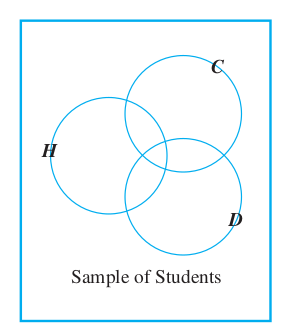
\includegraphics[scale=0.5]{../images/9.3.33.c.1.png}
\end{figure}

Let H be the set of students who checked \#1, C the set of students who checked \#2, and D the set of students who 
checked \#3. Fill in the numbers for all eight regions of the diagram.

\begin{proof}
\begin{figure}[ht!]
\centering
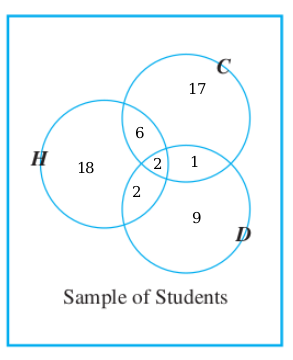
\includegraphics[scale=0.5]{../images/9.3.33.c.2.png}
\end{figure}
\end{proof}

\subsubsection{(d)}
How many students checked \#1 and \#2 but not \#3?

\begin{proof}
The number of students who checked \#1 and \#2 but not \#3 is \(N(H \cap D) - N(H \cap C \cap D) = 8 - 2 = 6\).
\end{proof}

\subsubsection{(e)}
How many students checked \#2 and \#3 but not \#1?

\begin{proof}
The number of students who checked \#2 and \#3 but not \#1 is \(N(C \cap D) - N(H \cap C \cap D) = 3 - 2 = 1\).
\end{proof}

\subsubsection{(f)}
How many students checked \#2 but neither of the other two?

\begin{proof}
The number of students who checked \#2 but not \#1 or \#3 is \(N(C) - N(C \cap (H \cup D)) = 17 - (6+2+1) = 8\).
\end{proof}

\subsection{Exercise 34}
A study was done to determine the efficacy of three different drugs: A, B, and C, in relieving headache pain. 
Over the period covered by the study, 50 subjects were given the chance to use all three drugs. The following 
results were obtained: 

21 reported relief from drug A

21 reported relief from drug B

31 reported relief from drug C

9 reported relief from both drugs A and B

14 reported relief from both drugs A and C

15 reported relief from both drugs B and C

41 reported relief from at least one of the drugs.

Note that some of the 21 subjects who reported relief from drug A may also have reported relief from drugs B or C. A 
similar occurrence may be true for the other data.

\subsubsection{(a)}
How many people got relief from none of the drugs?

\begin{proof}
\(50-41=9\)
\end{proof}

\subsubsection{(b)}
How many people got relief from all three drugs?

\begin{proof}
By the Inclusion-Exclusion Principle,
\[
N(A \cup B \cup C) = N(A) + N(B) + N(C) - N(A \cap B) - N(A \cap C) - N(B \cap C) + N(A \cap B \cap C).
\]
By using the values given in the problem, we get
\[
41 = 21 + 21 + 31 - 9 - 14 - 15 + N(A \cap B \cap C).
\]
Solving we get \(N(A \cap B \cap C) = 6\).
\end{proof}

\subsubsection{(c)}
\begin{figure}[ht!]
\centering
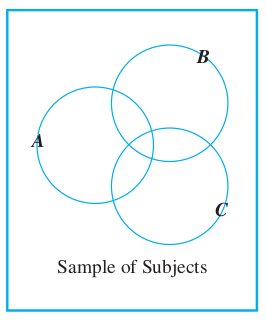
\includegraphics[scale=0.5]{../images/9.3.34.c.1.png}
\end{figure}

Let A be the set of all subjects who got relief from drug A, B the set of all subjects who got relief from drug B, 
and C the set of all subjects who got relief from drug C. Fill in the numbers for all eight regions of the diagram.

\begin{proof}
\begin{figure}[ht!]
\centering
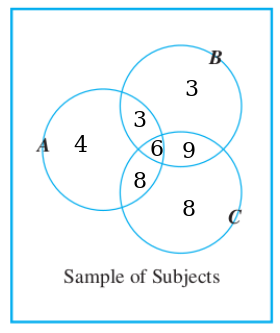
\includegraphics[scale=0.5]{../images/9.3.34.c.2.png}
\end{figure}
\end{proof}

\subsubsection{(d)}
How many subjects got relief from A only?

\begin{proof}
4
\end{proof}

\subsection{Exercise 35}
An interesting use of the inclusion/exclusion rule is to check survey numbers for consistency. For example, suppose 
a public opinion polltaker reports that out of a national sample of 1,200 adults, 675 are married, 682 are from 20 to 
30 years old, 684 are female, 195 are married and are from 20 to 30 years old, 467 are married females, 318 are 
females from 20 to 30 years old, and 165 are married females from 20 to 30 years old. Are the polltaker’s 
figures consistent? Could they have occurred as a result of an actual sample survey?

\begin{proof}
Let \(M\) = the set of married people in the sample,

\(Y\) = the set of people between 20 and 30 in the sample, and

\(F\) = the set of females in the sample.

Then the number of people in the set \(M \cup Y \cup F\) is less than or equal to the size of the sample. And so 

\begin{tabular}{rcl}
1,200 & \(\geq\) & \(N(M \cup Y \cup F)\) \\
& = & \(N(M) + N(Y) + N(F) - N(M \cap Y)\) \\
&   & \(-N(M \cap F) -N(Y \cap F) + N(M \cap Y \cap F)\) \\ 
& = & \(675 + 682 + 684 - 195 - 467 - 318 + 165\) \\
& = & 1,226.
\end{tabular}

This is impossible since \(1,200 < 1,226\), so the polltaker’s figures are inconsistent. They could not have 
occurred as a result of an actual sample survey.
\end{proof}

\subsection{Exercise 36}
Fill in the reasons for each step below. If $A$ and $B$ are sets in a finite universe $U$, then
\begin{center}
\begin{tabular}{rcll}
\(N(A \cap B)\) & = & \(N(U) - N((A \cap B)^c)\) & {\cy (a) \fbl} \\
& = & \(N(U) - N(A^c \cup B^c)\) & {\cy (b) \fbl} \\
& = & \(N(U) - (N(A^c) + N(B^c) - N(A^c \cap B^c))\) & {\cy (c) \fbl}
\end{tabular}
\end{center}
\begin{proof}
(a) because 
\begin{center}
\begin{tabular}{rcll}
\(A \cap B\) & = & \((A \cap B) \cap U\) & by identity law \\
& = & \(U \cap (A \cap B)\) & by commutative law \\
& = & \(U \cap ((A \cap B)^c)^c\) & by double complement law \\
& = & \(U - (A \cap B)^c\) & by set difference law \\
\end{tabular}
\end{center}
and because \(N(U - (A \cap B)^c) = N(U) - N((A \cap B)^c)\).

(b) by De Morgan laws (c) by inclusion-exclusion principle for 2 sets
\end{proof}

{\bf \cy For each of exercises $37-39$, the number of elements in a certain set can be found by computing the 
number in a larger universe that are not in the set and subtracting this from the total in the larger universe. In 
each of these, as was the case for the solution to example 9.3.6(b), De Morgan’s laws and the inclusion / exclusion 
rule can be used.}

\subsection{Exercise 37}
How many positive integers less than 1,000 have no common factors with 1,000?

\begin{proof}
Let $A$ be the set of all positive integers less than 1,000 that are not multiples of 2, and let $B$ be the set of all 
positive integers less than 1,000 that are not multiples of 5. Since the only prime factors of 1,000 are 2 and 5, the 
number of positive integers that have no common factors with 1,000 is \(N(A \cap B)\). Let the universe $U$ be the 
set of all positive integers less than 1,000. Then \(A^c\) is the set of positive integers less than 1,000 that are 
multiples of 2, \(B^c\) is the set of positive integers less than 1,000 that are multiples of 5, and \(A^c \cap 
B^c\) is the set of positive integers less than 1,000 that are multiples of 10. By one of the procedures discussed in 
Section 9.1 or 9.2, it is easily found that \(N(A^c) = 499, N(B^c) = 199\), and \(N(A^c \cap B^c) = 99\). Thus, by the 
inclusion/exclusion rule, \(N(A^c \cup B^c) = N(A^c) + N(B^c) - N(A^c \cap B^c) = 499 + 199 - 99 = 599\). But by 
De Morgan’s law, \(N(A^c \cup B^c) = N((A \cap B)^c)\), and so (*) \(N((A \cap B)^c) = 599\). Now since \((A \cap B)^c 
= U - (A \cap B)\), by the difference rule we have (**) \(N((A \cap B)^c) = N(U) - N(A \cap B)\). Equating the 
right-hand sides of (*) and (**) gives \(N(U) - N(A \cap B) = 599\). And because \(N(U) = 999\), we conclude that \(999 
- N(A \cap B) = 599\), or, equivalently, \(N(A \cap B) = 999 - 599 = 400\). So there are 400 positive integers less 
than 1,000 that have no common factor with 1,000.
\end{proof}

\subsection{Exercise 38}
How many permutations of \(abcde\) are there in which the first character is \(a, b\), or $c$ and the last character is \(c, d\), or $e$?

\begin{proof}
{\bf Case 1: first character is $a$.} For the last character there are 3 choices: \(c, d, e\). Then the middle
3 characters can be permuted in \(3!\) ways. So \(3 \cdot 3! = 3 \cdot 6 = 18\) possibilities.

{\bf Case 2: first character is $b$.} For the last character there are 3 choices: \(c, d, e\). Then the middle
3 characters can be permuted in \(3!\) ways. So \(3 \cdot 3! = 3 \cdot 6 = 18\) possibilities.

{\bf Case 3: first character is $c$.} For the last character there are 2 choices: \(d, e\). Then the middle
3 characters can be permuted in \(3!\) ways. So \(2 \cdot 3! = 2 \cdot 6 = 12\) possibilities.

In total, there are \(18+18+12 = 48\) permutations in which the first character is \(a, b\), or $c$ and the last 
character is \(c, d\), or $e$.
\end{proof}

\subsection{Exercise 39}
How many integers from 1 through 999,999 contain each of the digits 1, 2, and 3 at least once? ({\it Hint:} For each 
\(i = 1, 2\), and 3, let \(A_i\) be the set of all integers from 1 through 999,999 that do not contain the digit $i$.)

\begin{proof}
Let \(A_1, A_2, A_3\) be the sets of all integers from 1 through 999,999 that do not contain the digits 1, 2, 3,
respectively.

\(N(A_1) = 9^6 - 1\) because, excluding the digit 1, there are 9 choices for each digit, for a total of \(9^6\), but
one of them, namely 000,000 corresponds to 0 which is out of the range 1 through 999,999.

Similarly \(N(A_2) = N(A_3) = 9^6-1\).

\(N(A_1 \cap A_2) = 8^6 - 1\) because, excluding the digits 1 and 2, there are 8 choices for each digit, for a total of 
\(8^6\), but one of them, namely 000,000 corresponds to 0 which is out of the range 1 through 999,999.

Similarly \(N(A_1 \cap A_3) = N(A_2 \cap A_3) = 8^6 - 1\).

Finally \(N(A_1 \cap A_2 \cap A_3) = 7^6-1\) by a similar argument to the above arguments. 

Now by the inclusion / exclusion principle, \(N(A_1 \cup A_2 \cup A_3) = N(A_1) + N(A_2) + N(A_3) - N(A_1 \cap A_2) 
- N(A_1 \cap A_3) - N(A_2 \cap A_3) + N(A_1 \cap A_2 \cap A_3) = 3(9^6-1) - 3(8^6-1) + 7^6-1 = 925,539\)

So the number of integers that do not contain at least one of the digits 1,2,3 is 925,539. Then \(999,999 - 925,539 = 
74460\) integers contain all three of the digits 1,2,3.

We can verify this with a computer:
\begin{minted}{scala}
scala> var count = 0
var count: Int = 0
                                                                                                                        
scala> for i <- 1 to 999999 do
     |   if "123".forall(c => i.toString.contains(c)) then
     |     count += 1
     | 
scala> count
val res0: Int = 74460
\end{minted}
\end{proof}

{\bf \cy For 40 and 41, use the definition of the Euler phi function \(\phi\) from Section 7.1, exercises $51-53$.}

\subsection{Exercise 40}
Use the inclusion/exclusion principle to prove the following: If \(n = pq\), where $p$ and $q$ are distinct prime numbers, then \(\phi(n) = (p - 1)(q - 1)\).

{\it Hint:} Let $A$ and $B$ be the sets of all positive integers less than or equal to $n$ that are divisible by 
$p$ and $q$, respectively. Then \(\phi(n) = n - N(A \cup B)\).

\begin{proof}
(following the Hint) 

Notice \(N(A) = q\) since there are $q$ multiples of $p$ from 1 to $n$: \(p, 2p, 3p, \ldots, (q-1)p, qp = n\).
Similarly \(N(B) = p\).

Notice \(N(A \cap B) = 1\) since \(n = pq\) is the only number from 1 through $n$ that is divisible by both $p$ and $q$.

By the inclusion / exclusion principle, \(N(A \cup B) = N(A) + N(B) - N(A \cap B) = q + p - 1\). So \(\phi(n) = n - 
(q+p-1) = pq-q-p+1 = q(p-1) - (p-1) = (p-1)(q-1)\).
\end{proof}

\subsection{Exercise 41}
Use the inclusion/exclusion principle to prove the following: If \(n = pqr\), where \(p, q\), and \(r\) are 
distinct prime numbers, then \(\phi(n) = (p - 1)(q - 1)(r - 1)\).

\begin{proof}
We can use an approach similar to Exercise 40. Let \(P, Q, R\) be the sets of positive integers less than or equal to
$n$ that are divisible by \(p,q,r\) respectively. 

Then \(N(P) = qr, N(Q) = pr, N(R) = pq\) by similar arguments. 

Now \(N(P \cap Q) = r\) because: if an integer is divisible by both $p$ and $q$ then it is divisible by $pq$ since $p$ 
and $q$ are both prime; and there are $r$ multiples of $pq$ from 1 through $n$: \(pq, 2pq, 3pq, \ldots, (r-1)pq, rpq = n\).

By similar arguments \(N(P \cap R) = q\) and \(N(Q \cap R) = p\). Finally \(N(P \cap Q \cap R) = 1\) because \(n=pqr\)
itself is the only integer divisible by all 3 primes.

By the inclusion / exclusion principle, \(N(P \cup Q \cup R) = N(P) + N(Q) + N(R) - N(P \cap Q) -N(P \cap R) - N(Q 
\cap R) + N(P \cap Q \cap R) = qr + pr + pq - r - q - p + 1\).

\(N(P \cup Q \cup R)\) is the number of integers that are divisible by at least one of \(p,q,r\), thus \(\phi(n) = 
n - N(P \cup Q \cup R) = pqr - qr + pr + pq - r - q - p + 1\), which, after factoring, equals \((p-1)(q-1)(r-1)\).
\end{proof}

\subsection{Exercise 42}
A gambler decides to play successive games of blackjack until he loses three times in a row. (Thus the gambler 
could play five games by losing the first, winning the second, and losing the final three or by winning the first 
two and losing the final three. These possibilities can be symbolized as LWLLL and WWLLL.) Let \(g_n\) be the number 
of ways the gambler can play $n$ games.

\subsubsection{(a)}
Find \(g_3, g_4\), and \(g_5\).

\begin{proof}
3 games: LLL so \(g_3 = 1\). \,\,\, 4 games: WLLL so \(g_4 = 1\). 

5 games: LWLLL, WWLLL so \(g_5 = 2\).
\end{proof}

\subsubsection{(b)}
Find \(g_6\).

\begin{proof}
6 games: WWWLLL, LWWLLL, WLWLLL, LLWLLL so \(g_6 = 4\).
\end{proof}

\subsubsection{(c)}
Find a recurrence relation for \(g_3, g_4, g_5, \ldots\).

{\it Hint:} If \(k \geq 6\), any sequence of $k$ games must begin with W, LW, or LLW.

\begin{proof}
By the Hint we can see that for \(k \geq 6, g_k = g_{k-1} + g_{k-2} + g_{k-3}\).
\end{proof}

\subsection{Exercise 43}
A derangement of the set \(\{1, 2, \ldots, n\}\) is a permutation that moves every element of the set away from 
its “natural” position. Thus 21 is a derangement of \(\{1, 2\}\), and 231 and 312 are derangements of \(\{1, 2, 3\}\). 
For each positive integer $n$, let \(d_n\) be the number of derangements of the set \(\{1, 2, \ldots, n\}\).

\subsubsection{(a)}
Find \(d_1, d_2\), and \(d_3\).

\begin{proof}
\(d_1 = 0\) because the only permutation of the set \(\{1\}\) is 1, which cannot move 1 from its natural position.

\(d_2 = 1\) because the only two permutations of the set \(\{1,2\}\) are 12 and 21, and only 21 moves both 1 and 2 
away from their natural positions.

\(d_3 = 2\) because there are 6 permutations of the set \(\{1,2,3\}\): 123, 132, 213, 231, 312, 321; and only 231 
and 312 move every element away from their natural positions.
\end{proof}

\subsubsection{(b)}
Find \(d_4\).

\begin{proof}
There are 24 permutations: 1234, 1243, 1324, 1342, 1423, 1432, 2134, 2143, 2314, 2341, 2413, 2431, 3124, 3142, 3214, 
3241, 3412, 3421, 4123, 4132, 4213, 4231, 4312, 4321.

The only ones that move every element away from their natural positions are: 2143, 2341, 2413, 3142, 3412, 3421, 
4123, 4312, 4321.

So \(d_4 = 9\).
\end{proof}

\subsubsection{(c)}
Find a recurrence relation for \(d_1, d_2, d_3, \ldots\).

{\it Hint:} Divide the set of all derangements into two subsets: one subset consists of all derangements in which 
the number 1 changes places with another number, and the other subset consists of all derangements in which the 
number 1 goes to position \(i \neq 1\) but $i$ does not go to position 1. The answer is \(d_k = (k - 1)d_{k-1} + (k-1)
d_{k-2}\). Can you justify it?

\begin{proof}
(following the Hint) 

Consider a derangement in the first subset. Then 1 switches places with another number $i$. There are $k-1$ other 
numbers that 1 can switch places with. For each one of them, then the remaining \(k-2\) numbers have to also 
derange, and there are \(d_{k-2}\) ways to do that. Thus the number of derangements in the first subset is 
\((k-1)d_{k-2}\).

Consider a derangement in the second subset. Then 1 moves to position $i$ for some number $i$. There are $k-1$ 
choices for this $i$. For each one of these choices, there are \(d_{k-1}\) ways to derange the remaining $k-1$ 
numbers. Why? 

Because number $i$ cannot go to position 1, but it can go to any one of the remaining $k-2$ positions, and similarly 
any other number $j$ (\(j \neq 1, j \neq i\)) can go to $k-2$ positions (any position except $j$ and $i$), so this 
situation is the same as derangements of $k-1$ elements. 

Thus the number of derangements in the second subset is \((k-1)d_{k-1}\). So the total is: 
\(d_k = (k - 1)d_{k-1} + (k - 1)d_{k-2}\).
\end{proof}

\subsection{Exercise 44}
Note that a product \(x_1x_2x_3\) may be parenthesized in two different ways: \((x_1x_2)x_3\) and \(x_1(x_2x_3)\). 
Similarly, there are several different ways to parenthesize \(x_1x_2x_3x_4\). Two such ways are \((x_1x_2)(x_3x_4)\) 
and \(x_1((x_2 x_3)x_4)\). Let \(P_n\) be the number of different ways to parenthesize the product \(x_1x_2 \ldots 
x_n\). Show that if \(P_1 = 1\), then 
\[
P_n = \sum_{k=1}^{n-1} P_k P_{n-k} \text{ for every integer  } n \geq 2. 
\]
(It turns out that the sequence \(P_1, P_2, P_3, \ldots\) is the same as the sequence of Catalan numbers: 
\(P_n = C_{n-1}\) for every integer \(n \geq 1\). See Example 5.6.4.)

\begin{proof}
Consider the product \(x_1x_2 \ldots x_n\). All the different ways to parenthesize it can be classified as 
follows: split it into two products \(x_1\) and \(x_2 \ldots x_n\), or into \(x_1x_2\) and \(x_3 \ldots x_n\),
or into \(x_1x_2x_3\) and \(x_4 \ldots x_n\), \(\ldots\), or into \(x_1x_2 \ldots x_{n-1}\) and \(x_n\).

By the addition rule, $P_n$ is the sum of the number of ways each one of these product pairs can be parenthesized.

For each of the product pairs, by the product rule, the number of ways to parenthesize the product pair is the 
product of the numbers of ways to parenthesize each product.

There are \(P_1\) ways to parenthesize \(x_1\) and \(P_{n-1}\) ways to parenthesize \(x_2 \ldots x_n\), so 
there are \(P_1P_{n-1}\) ways to parenthesize their product.

Similarly there are \(P_2\) ways to parenthesize \(x_1x_2\) and \(P_{n-2}\) ways to parenthesize \(x_3 \ldots x_n\), so 
there are \(P_2P_{n-2}\) ways to parenthesize their product.

And so on. Therefore \(P_n = \sum_{k=1}^{n-1} P_k P_{n-k}\) for every \(n \geq 2\).
\end{proof}

\subsection{Exercise 45}
Use mathematical induction to prove Theorem 9.3.1: ``Suppose a finite set $A$ equals the union of $k$ distinct 
mutually disjoint subsets \(A_1, A_2, \ldots, A_k\). Then \(N(A) = N(A_1) + N(A_2) + \ldots + N(A_k)\).''

\begin{proof}
Let \(P(n)\) be the statement ``if a finite set $A$ equals the union of $n$ distinct mutually disjoint subsets 
\(A_1, A_2, \ldots, A_n\) then \(N(A) = N(A_1) + N(A_2) + \cdots + N(A_n)\).''

{\bf Show that \(P(1)\) is true:} In this case \(A = A_1\) therefore \(N(A) = N(A_1)\), so \(P(1)\) is true.

{\bf Show that for any integer \(k \geq 1\) if \(P(k)\) is true then \(P(k+1)\) is true:} Assume \(P(k)\) is true and 
assume \(A\) is a finite set that equals the union of $k+1$ mutually disjoint subsets \(A_1, \ldots, A_k, A_{k+1}\).
{\it [We want to show \(N(A) = N(A_1) + N(A_2) + \cdots + N(A_{k+1})\)]}.

Let \(A' = A_1 \cup \cdots \cup A_k\). Then \(A'\) is a finite set that equals the union of $k$ mutually disjoint 
subsets \(A_1, \ldots, A_k\). By the inductive hypothesis \(N(A') = N(A_1) + N(A_2) + \cdots + N(A_k)\).

Notice that since \(A_1, \ldots, A_{k+1}\) are mutually disjoint, \(A' = A_1 \cup \cdots \cup A_k\) and \(A_{k+1}\) 
are also disjoint. So \(N(A) = N(A' \cup A_{k+1}) = N(A') + N(A_{k+1})=N(A_1) +N(A_2) + \cdots + N(A_k) + N(A_{k+1})\), 
{\it [as was to be shown.]}
\end{proof}

\subsection{Exercise 46}
Prove the inclusion/exclusion rule for two sets $A$ and $B$ by showing that \(A \cup B\) can be partitioned into 
\(A \cap B\), \(A - (A \cap B)\), and \(B - (A \cap B)\), and then using the addition and difference rules. 
(See the hint for exercise 39 in Section 6.2.)

\begin{proof}
{\bf Claim:} \(A \cup B = (A \cap B) \cup [A - (A \cap B)] \cup [B - (A \cap B)]\) and \((A \cap B), A-(A \cap B)\) 
and \(B-(A \cap B)\) are mutually disjoint sets.

{\it Proof of Claim.} 

{\it First to prove the equality:}

1. Assume \(x \in A \cup B\). 

2. By definition of union, \(x \in A\) or \(x \in B\).

3. {\bf Case 1: \(x \in A\).}

3.1 {\bf Case 1.1: \(x \in B\).} Then by definition of intersection, \(x \in A \cap B\). So by definition of union
\(x \in (A \cap B) \cup [A - (A \cap B)] \cup [B - (A \cap B)]\).

3.2 {\bf Case 1.2: \(x \notin B\).} Then by definition of intersection, \(x \notin A \cap B\). So by definition of 
difference \(x \in A - (A \cap B)\). So by definition of union, \(x \in (A \cap B) \cup [A - (A \cap B)] \cup 
[B - (A \cap B)]\).

4. {\bf Case 2: \(x \in B\).} Similar to Case 1. We conclude \(x \in (A \cap B) \cup [A - (A \cap B)] \cup 
[B - (A \cap B)]\).

5. By 3 and 4, \(x \in (A \cap B) \cup [A - (A \cap B)] \cup [B - (A \cap B)]\).

6. By 1, 5 and definition of subset, \(A \cup B \subseteq (A \cap B) \cup [A - (A \cap B)] \cup [B - (A \cap B)]\).

7. Assume \(x \in (A \cap B) \cup [A - (A \cap B)] \cup 
[B - (A \cap B)]\).

8. By definition of union, \(x \in A \cap B\) or \(x \in A - (A \cap B)\) or \(x \in B - (A \cap B)\).

9. {\bf Case 1: \(x \in A \cap B\).} By definition of intersection \(x \in A\) and \(x \in B\). So by definition
of union, \(x \in A \cup B\).

10. {\bf Case 2: \(x \in A - (A \cap B)\).} By definition of difference, \(x \in A\) and \(x \notin A \cap B\). So by 
definition of union, \(x \in A \cup B\).

11. {\bf Case 3: \(x \in B - (A \cap B)\).} By definition of difference, \(x \in B\) and \(x \notin A \cap B\). So by 
definition of union, \(x \in A \cup B\).

12. By 9, 10 and 11, \(x \in A \cup B\).

13. By 7, 12 and definition of subset, \((A \cap B) \cup [A - (A \cap B)] \cup [B - (A \cap B)] \subseteq A \cup B\).

14. By 6, 13 and definition of set equality \((A \cap B) \cup [A - (A \cap B)] \cup [B - (A \cap B)] = A \cup B\).

{\it Now to prove that the three sets are mutually disjoint:}

Assume \(x \in A \cap B\). We want to show \(x \notin A - (A \cap B)\) and \(x \notin B - (A \cap B)\). 

Argue by contradiction and assume \(x \in A - (A \cap B)\). Then by definition of difference \(x \in A\) and \(x \notin 
A \cap B\), contradicting \(x \in A\cap B\). Similarly we can prove \(x \notin B - (A \cap B)\).

Assume \(x \in A - (A \cap B)\). We want to show \(x \notin A \cap B\) and \(x \notin B - (A \cap B)\). 

By definition of difference, \(x \in A\) and \(x \notin A \cap B\). Then by definition of intersection either 
\(x \notin A\) or \(x \notin B\). The first case \(x \notin A\) contradicts the fact that \(x\in A\), so \(x\notin B\). 
So by definition of intersection \(x \notin A \cap B\) (otherwise \(x \in B\), contradiction) and by definition of 
difference \(x \notin B - (A \cap B)\) either (otherwise \(x \in B\), contradiction).

Assume \(x \in B - (A \cap B)\). We want to show \(x \notin A \cap B\) and \(x \notin A - (A \cap B)\). This proof is 
very similar to the case above.

{\it [end of proof of the Claim.]}

By the claim \(N(A \cup B) = N((A \cap B) \cup [A - (A \cap B)] \cup [B - (A \cap B)])\).

Since these sets are disjoint by the claim, by the addition rule \(N(A \cup B) = N(A \cap B) + N(A - (A \cap B)) + N(B 
- (A \cap B)).\)

By the difference rule \(N(A - (A \cap B)) = N(A) - N(A \cap B)\) and \(N(B - (A \cap B)) = N(B) - N(A \cap B)\).
Substituting these into the equation above, we get
\[
N(A \cup B) = N(A \cap B) + N(A) - N(A \cap B) + N(B) - N(A \cap B) = N(A) + N(B) - N(A \cap B)
\]
{\it [which proves the Inclusion / Exclusion principle for two sets.]}
\end{proof}

\subsection{Exercise 47}
Prove the inclusion/exclusion rule for three sets.

\begin{proof}
Let \(A,B,C\) be any sets. {\it [We want to show that]}
\[
N(A \cup B \cup C) = N(A) + N(B) + N(C) - N(A \cap B) - N(A \cap C) - N(B \cap C) + N(A \cap B \cap C).
\]
By the Inclusion / Exclusion Principle for two sets, applied to the two sets \(A \cup B\) and \(C\),
\[
N((A \cup B) \cup C) = N(A \cup B) + N(C) - N((A \cup B) \cap C) \hspace{2cm} (1)
\]
By the Inclusion / Exclusion Principle for two sets, applied to the two sets \(A\) and \(B\),
\[
N(A \cup B) = N(A) + N(B) - N(A \cap B) \hspace{2cm} (2)
\]
By the distributive law \((A \cup B) \cap C = (A \cap C) \cup (B \cap C)\). By Inclusion / Exclusion again, 
\[
N((A \cap C) \cup (B \cap C)) = N(A \cap C) + N(B \cap C) - N((A \cap C) \cap (B \cap C)) \hspace{1cm} (3)
\]
Notice \((A \cap C) \cap (B \cap C) = A \cap B \cap C\). Substituting this together with (2) and (3) into (1) we get
\(N((A \cup B) \cup C)\)
\begin{center}
\begin{tabular}{cl}
= & \(N(A \cup B) + N(C) - N((A \cup B) \cap C)\) \\
= & \([N(A) + N(B) - N(A \cap B)] + N(C) - N((A \cap C) \cup (B \cap C))\) \\
= & \([N(A) + N(B) - N(A \cap B)] + N(C) - [N(A \cap C) + N(B \cap C) - N(A \cap B \cap C)]\) \\
= & \(N(A) + N(B) + N(C) - N(A \cap B) - N(A \cap C) - N(B \cap C) + N(A \cap B \cap C)\) \\
\end{tabular}
\end{center}
{\it [as was to be shown.]}
\end{proof}

\subsection{Exercise 48}
Use mathematical induction to prove the general inclusion/exclusion rule: If \(A_1, \ldots, A_n\) are finite sets, 
then \(N(A_1 \cup A_2 \cup \cdots \cup A_n)\)
\begin{center}
\begin{tabular}{l}
= \(\dps \sum_{1 \leq i \leq n}N(A_i) - \sum_{1 \leq i < j \leq n} N(A_i \cap A_j) + \sum_{1 \leq i < j < k \leq n} 
N(A_i \cap A_j \cap A_k)\) \\
\(\dps - \cdots + (-1)^{n+1} N(A_1 \cap A_2 \cap \cdots \cap A_n)\) 
\end{tabular}
\end{center}
(The notation \(\sum_{1 \leq i < j \leq n} N(A_i \cap A_j)\) means that quantities of the form \(N(A_i \cap A_j)\) 
are to be added together for all integers $i$ and $j$ with \(1 \leq i < j \leq n\).)

{\it Hint:} Use the associative law for sets from Theorem 6.2.2 and the generalized distributive law for sets from 
exercise 40, Section 6.2.

\begin{proof}
Let \(P(n)\) be the statement: ``if \(A_1, \ldots, A_n\) are finite sets then the equation above is true.''

{\bf Show that \(P(1)\) is true:} When \(n=1\) the equation becomes \(N(A_1) = \sum_{1 \leq i \leq 1} N(A_1)\), with 
all the other sums becoming empty sums, since \(1 \leq i < j \leq 1\) is impossible for integers $i,j$. Both sides are
equal to \(N(A_1)\) therefore $P(1)$ is true.

{\bf Show that for any integer \(n \geq 1\) if \(P(n)\) is true then \(P(n+1)\) is true:} Assume \(n \geq 1\) and 
assume \(P(n)\) is true. Assume \(A_1, \ldots, A_{n+1}\) are finite sets. {\it [We want to prove \(P(n+1)\).]}

Let \(B = \bigcup_{i=1}^n A_i\). Notice \(\bigcup_{i=1}^{n+1}A_i = B \cup A_{n+1}\). Then by the inclusion / exclusion principle for two sets,
\[
N\left(\bigcup_{i=1}^{n+1}A_i\right) = N(B \cup A_{n+1}) = N(B) + N(A_{n+1}) - N(B \cap A_{n+1}) \hspace{2cm} (1)
\]
By the inductive hypothesis
\[
N(B) = \sum_{1 \leq i \leq n} N(A_i) - \sum_{1 \leq i < j \leq n} N(A_i \cap A_j) + \cdots + (-1)^{n+1} N(A_1 \cap A_2 \cap \cdots \cap A_n) \,\,\, (2)
\]
By the generalized distributive law,
\[
B \cap A_{n+1} = (A_1 \cap A_{n+1}) \cup (A_2 \cap A_{n+1}) \cup \cdots \cup (A_k \cap A_{n+1}) = \bigcup_{i=1}^{n} 
(A_i \cap A_{n+1})
\]
By the inductive hypothesis again, \(N(B \cap A_{n+1}) = N\left(\bigcup_{i=1}^{n} (A_i \cap A_{n+1}) \right)\)
\begin{center}
\begin{tabular}{l}
= \(\dps \sum_{1 \leq i \leq n} N(A_i \cap A_{n+1}) - \sum_{1 \leq i < j \leq n} N((A_i \cap A_{n+1}) \cap 
(A_j \cap A_{n+1}))\) \\
\(\dps + \cdots + (-1)^{n+1}N\left(\bigcap_{i=1}^n (A_i \cap A_{n+1})\right)\) \hspace{4cm} (3)
\end{tabular}
\end{center}
Now let's try to substitute and combine all the terms. 

The term \(N(B)\) in (1) will be replaced by the right hand side of (2), and the term \(N(B \cap A_{n+1})\) in (1) will
be replaced by the right hand side of (3). So let's imagine we've done that already, and start combining terms in (1).

The term \(\dps \sum_{1 \leq i \leq n} N(A_i)\) on the right hand side of (2), and the term \(N(A_{n+1})\) in (1), 
can be combined into: \(\dps \sum_{1 \leq i \leq n+1} N(A_i)\).

The term \(\dps\sum_{1 \leq i < j \leq n} N(A_i \cap A_j)\) in (2) and the term \(\dps\sum_{1 \leq i \leq n} N(A_i \cap 
A_{n+1})\) on the right side of (3) can be combined into \(\dps\sum_{1 \leq i < j \leq n+1} N(A_i \cap A_j)\). Why? 
The first sum has all the two-way intersections between all the \(A_i\) from 1 to $n$, and the second sum has all the 
two-way intersections of the \(A_i\) from 1 to $n$ with \(A_{n+1}\). Putting them together we end up with all 
the two-way intersections between all the \(A_i\) from 1 to $n+1$. Both of these sums have negative signs (the second 
sum gets a negative sign from \(N(B \cap A_{n+1})\)).

Notice that the next term in (3) is, by the associative law and the idempotent law for intersection:
\[
\sum_{1 \leq i < j \leq n} N((A_i \cap A_{n+1}) \cap (A_j \cap A_{n+1})) = \sum_{1 \leq i < j \leq n} N(A_i \cap 
A_j \cap A_{n+1})
\]

So, similarly the term \(\dps \sum_{1 \leq i < j < k \leq n} N(A_i \cap A_j \cap A_k)\) in (2) and the term \(\dps 
\sum_{1 \leq i < j \leq n} N(A_i \cap A_j \cap A_{n+1})\) in (3) can be combined into \(\dps \sum_{1 \leq i < j < k 
\leq n+1} N(A_i \cap A_j \cap A_k)\) because the first sum has all the three-way intersections between \(A_i\) from 1 
to $n$, and the second sum has all the three-way intersections of \(A_{n+1}\) with the $A_i$ from 1 to $n$.
Both sums have a positive sign (the second sum has a double negative sign, one from \(N(B \cap A_{n+1})\) in (1) and
another from itself).

All the other $i$-way intersection term sums from (2) and (3) can be combined in a similar way. So we end up with: 
\(\dps N\left(\bigcup_{i=1}^{n+1}A_i\right)\)
\begin{center}
\begin{tabular}{l}
= \(\dps \sum_{1 \leq i \leq n+1}N(A_i) - \sum_{1 \leq i < j \leq n+1} N(A_i \cap A_j) + \sum_{1 \leq i < j < k \leq 
n+1} N(A_i \cap A_j \cap A_k)\) \\
\(\dps - \cdots + (-1)^{n+2} N(A_1 \cap A_2 \cap \cdots \cap A_{n+1})\) 
\end{tabular}
\end{center}
which proves \(P(n+1)\), {\it [as was to be shown.]}
\end{proof}

\subsection{Exercise 49}
A circular disk is cut into $n$ distinct sectors, each shaped like a piece of pie and all meeting at the center 
point of the disk. Each sector is to be painted red, green, yellow, or blue in such a way that no two adjacent sectors 
are painted the same color. Let \(S_n\) be the number of ways to paint the disk.

\subsubsection{(a)}
Find a recurrence relation for \(S_k\) in terms of \(S_{k-1}\) and \(S_{k-2}\) for each integer \(k \geq 4\).

{\it Hint:} Use the solution method described in Section 5.8. The answer is \(S_k = 2S_{k-1} + 3S_{k-2}\) for every 
integer \(k \geq 4\).

\begin{proof}
NOTE: I have to assume, without any extra information, that the disk is FIXED, in other words, rotation, flipping etc.
are considered different ways to paint.

For example, for \(n=3\) consider the clockwise paintings starting from the sector that occupies 12 o'clock: 

RGB and RBG: in both paintings, R is adjacent to G and B, G is adjacent to R and B, B is adjacent to R and G. In 
another way, they are equivalent if we traverse the second disk counter-clockwise.

YBG and BGY: These would be equivalent if rotation is allowed, because it amounts to choosing a different starting point.

{\it On to the problem:}

Consider a disk cut into \(k\) sectors and painted as described in the problem. Number the sectors as \(s_1, s_2, 
\ldots, s_k\). So \(s_k\) and \(s_1\) are adjacent, therefore of different colors. There are two cases: either 
\(s_1\) and \(s_{k-1}\) are painted the same color, or not.

{\bf Case 1: \(s_1\) and \(s_{k-1}\) are painted the same color.} In this case \(s_k\) can be painted one of the 
other 3 colors. Now remove \(s_k\) from the disk. The remaining \(k-1\) sectors can be considered a disk of 
\(k-2\) sectors, by merging \(s_1\) and \(s_{k-1}\) (since they are painted the same color). There are \(S_{k-2}\) 
ways to color this remaining disk. Therefore there are \(3S_{k-2}\) ways to color the original \(k\)-sector disk.

{\bf Case 2: \(s_1\) and \(s_{k-1}\) are painted different colors.} In this case \(s_k\) can be painted with one of 
the remaining 2 colors. Now remove \(s_k\) from the disk. The remaining \(k-1\) sectors form a valid painting by 
making \(s_1\) and \(s_{k-1}\) adjacent (since they are painted with different colors). There are \(S_{k-1}\) ways 
to paint this remaining disk. Therefore there are \(2S_{k-1}\) ways to color the original \(k\)-sector disk.

By the addition rule \(S_k = 2S_{k-1} + 3S_{k-2}\).
\end{proof}

\subsubsection{(b)}
Find an explicit formula for \(S_n\) for \(n \geq 2\).

\begin{proof}
\(S_2 = 12\) because there are 4 colors to paint \(s_1\), 3 colors to paint \(s_2\).

\(S_3 = 24\) because there are 4 colors to paint \(s_1\), 3 colors to paint \(s_2\), and, since \(s_3\) is adjacent to 
both \(s_1\) and \(s_2\), there are 2 colors to paint \(s_3\).

The characteristic equation is \(t^2 - 2t - 3 = 0\) so \((t-3)(t+1) = 0\) which gives \(t = -1, 3\). So the general
form of the solution is \(S_n = A \cdot (-1)^n + B \cdot 3^n\).

Solving \(S_2 = 12 = A(-1)^2 + B \cdot 3^2\) we get \(12 = A + 9B\). Solving \(S_3 = 24 = A(-1)^3 + B \cdot 3^3\) we get \(24 = -A + 27B\). Adding these two equations together gives \(36 = 36B\) so \(B = 1\) and \(A = 3\). 

Thus \(S_n = 3\cdot(-1)^n + 3^n\) for all \(n \geq 2\).
\end{proof}

\section{Exercise Set 9.4}

\subsection{Exercise 1}
\subsubsection{(a)}
If 4 cards are selected from a standard 52-card deck, must at least 2 be of the same suit? Why?

\begin{proof}
No. For instance, the aces of the four different suits could be selected.
\end{proof}

\subsubsection{(b)}
If 5 cards are selected from a standard 52-card deck, must at least 2 be of the same suit? Why?

\begin{proof}
Yes. Let \(x_1,x_2,x_3,x_4,x_5\) be five cards. Consider the function \(S\) that sends each card to its suit.

\begin{figure}[ht!]
\centering
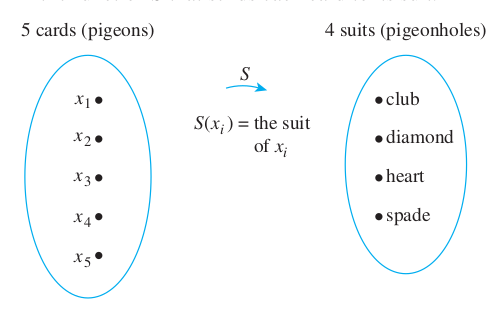
\includegraphics[scale=0.5]{../images/9.4.1.b.png}
\end{figure}

By the pigeonhole principle, \(S\) is not one-to-one: \(S(x_i) = S(x_j)\) for some two cards \(x_i\) and \(x_j\). 
Hence at least two cards have the same suit.
\end{proof}

\subsection{Exercise 2}
\subsubsection{(a)}
If 13 cards are selected from a standard 52-card deck, must at least 2 be of the same denomination? Why?

\begin{proof}
No, for example the 13 selected cards might have these denominations: 2, 3, 4, 5, 6, 7, 8, 9, 10, J, Q, K, A.
\end{proof}

\subsubsection{(b)}
If 20 cards are selected from a standard 52-card deck, must at least 2 be of the same denomination? Why?

\begin{proof}
Yes, since \(20 > 13\) and there are only 13 distinct denominations, by the Pigeonhole Principle at least 2 of 
them must be the same.
\end{proof}

\subsection{Exercise 3}
A small town has only 500 residents. Must there be 2 residents who have the same birthday? Why?

\begin{proof}
Yes. Denote the residents by \(x_1, x_2, \ldots, x_{500}\). Consider the function \(B\) from residents to birthdays 
that sends each resident to his or her birthday:

\begin{figure}[ht!]
\centering
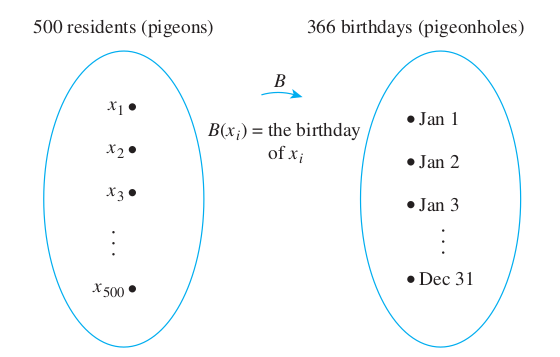
\includegraphics[scale=0.5]{../images/9.4.3.png}
\end{figure}

By the pigeonhole principle, \(B\) is not one-to-one: \(B(x_i) = B(x_j)\) for some two residents \(x_i\) and 
\(x_j\). Hence at least two residents have the same birthday.
\end{proof}

\subsection{Exercise 4}
In a group of 700 people, must there be 2 who have the same first and last initials? Why?

\begin{proof}
There are 26 letters in the Roman Alphabet, so there are \(26 \cdot 26 = 676\) possibilities for a first and last
initials combination. Since \(700 > 676\), by the Pigeonhole Principle at least 2 people must have the same initials.
\end{proof}

\subsection{Exercise 5}
\subsubsection{(a)}
Given any set of four integers, must there be two that have the same remainder when divided by 3? Why?

\begin{proof}
Yes. There are only three possible remainders that can be obtained when an integer is divided by 3: 0, 1, and 2. 
Thus, by the pigeonhole principle, if four integers are each divided by 3, then at least two of them must have the 
same remainder. More formally, call the integers \(n_1, n_2, n_3\), and \(n_4\), and consider the function \(R\) 
that sends each integer to the remainder obtained when that integer is divided by 3:

\begin{figure}[ht!]
\centering
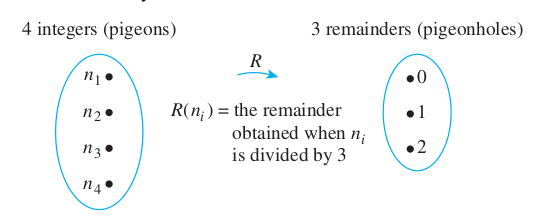
\includegraphics[scale=0.5]{../images/9.4.5.a.png}
\end{figure}

By the pigeonhole principle, \(R\) is not one-to-one: \(R(n_i) = R(n_j)\) for some two integers \(n_i\) and 
\(n_j\). Hence at least two integers must have the same remainder.
\end{proof}

\subsubsection{(b)}
Given any set of three integers, must there be two that have the same remainder when divided by 3? Why?

\begin{proof}
No. For instance, \(\{0, 1, 2\}\) is a set of three integers no two of which have the same remainder when 
divided by 3.
\end{proof}

\subsection{Exercise 6}
\subsubsection{(a)}
Given any set of seven integers, must there be two that have the same remainder when divided by 6? Why?

\begin{proof}
Yes. The possible remainders are 0, 1, 2, 3, 4, 5 and there are 6 possibilities. Since \(7 > 6\), by the Pigeonhole 
Principle at least two of the seven integers must have the same remainder. More formally we can think of \(\mod 6\) as 
a function defined on the set of seven integers: \(M: \{x_1 ,x_2,x_3,x_4 , x_5 , x_6 , x_7\} \to \{0, 1, 2, 3, 4, 5\}\) 
and \(M\) is not one-to-one because the domain has 7 elements while the range only has 6.
\end{proof}

\subsubsection{(b)}
Given any set of seven integers, must there be two that have the same remainder when divided by 8? Why?

\begin{proof}
No, for example \(\{0, 1, 2, 3, 4, 5, 6, 7\}\) is a set of seven integers no two of which have the same remainder.
\end{proof}

\subsection{Exercise 7}
Let \(S = \{3, 4, 5, 6, 7, 8, 9, 10, 11, 12\}\). Suppose six integers are chosen from \(S\). Must there be two 
integers whose sum is 15? Why?

\begin{proof}
Notice that \(3 + 12 = 15\), \(4 + 11 = 15\), \(5 + 10 = 15\), \(6 + 9 = 15\), and \(7 + 8 = 15\). 

We can divide \(S\) into five sets: \(\{3, 12\}\), \(\{4, 11\}\), \(\{5, 10\}\), \(\{6, 9\}\), \(\{7, 8\}\). 

By the Pigeonhole Principle, when 6 integers are chosen from \(S\), two of them will belong to the same set among 
these 5 sets. Therefore when 6 integers are chosen from \(S\) there must be two integers whose sum is 15.
\end{proof}

\subsection{Exercise 8}
Let \(T = \{1, 2, 3, 4, 5, 6, 7, 8, 9\}\). Suppose five integers are chosen from \(T\). Must there be two integers 
whose sum is 10? Why?

\begin{proof}
No, for example \(\{1,2,3,4,5\}\) contains no two integers whose sum is 10.
\end{proof}

\subsection{Exercise 9}
\subsubsection{(a)}
If seven integers are chosen from between 1 and 12 inclusive, must at least one of them be odd? Why?

\begin{proof}
Yes.

{\it Solution 1:} Only six of the numbers from 1 to 12 are even (namely, 2, 4, 6, 8, 10, 12), so at most six even 
numbers can be chosen from between 1 and 12 inclusive. Hence if seven numbers are chosen, at least one must be odd.

{\it Solution 2:} Partition the set of all integers from 1 through 12 into six subsets (the pigeonholes), each 
consisting of an odd and an even number: \(\{1, 2\}\), \(\{3, 4\}\), \(\{5, 6\}\), \(\{7, 8\}\), \(\{9, 10\}\), 
\(\{11, 12\}\). If seven integers (the pigeons) are chosen from among 1 through 12, then, by the pigeonhole principle, 
at least two must be from the same subset. But each subset contains one odd and one even number. Hence at least one of 
the seven numbers is odd.

{\it Solution 3: (a formal version of Solution 2):} Let
\(S = \{x_1, x_2, x_3, x_4, x_5, x_6, x_7\}\) be a set of 
seven numbers chosen from the set \(T = \{1, 2, 3, 4, 5, 6, 7, 8, 9, 10, 11, 12\}\), and let \(P\) be the following 
partition of \(T: \{1, 2\}, \{3, 4\}, \{5, 6\}, \{7, 8\}, \{9, 10\}\), and \(\{11, 12\}\). Since each element of 
\(S\) lies in exactly one subset of the partition, we can define a function \(F\) from \(S\) to \(P\) by letting 
\(F(x_i)\) be the subset that contains \(x_i\).

\begin{figure}[ht!]
\centering
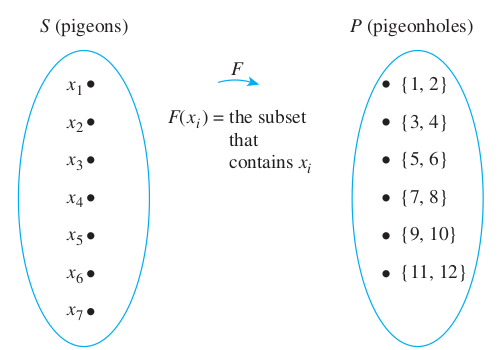
\includegraphics[scale=0.5]{../images/9.4.9.a.png}
\end{figure}

Since \(S\) has 7 elements and \(P\) has 6 elements, by the pigeonhole principle, \(F\) is not one-to-one. Thus two 
distinct numbers of the seven are sent to the same subset, which implies that these two numbers are the two distinct 
elements of the subset. Therefore, since each pair consists of one odd and one even integer, one of the seven numbers 
is odd.
\end{proof}

\subsubsection{(b)}
If ten integers are chosen from between 1 and 20 inclusive, must at least one of them be even? Why?

\begin{proof}
No. For instance, none of the 10 numbers 1, 3, 5, 7,
9, 11, 13, 15, 17, 19 is even.
\end{proof}

\subsection{Exercise 10}
If \(n + 1\) integers are chosen from the set \(\{1, 2, 3, \ldots, 2n\}\), where \(n\) is a positive integer, must at 
least one of them be odd? Why?

\begin{proof}
Yes. There are \(n\) even integers in the set \(\{1, 2, 3, \ldots, 2n\}\), namely, \(2(= 2 \cdot 1), 4(= 2 \cdot 2)\), \(6(= 2 \cdot 3), \ldots, 2n(= 2 \cdot n)\). So the maximum number of even integers that can be chosen is \(n\). Thus 
if \(n + 1\) integers are chosen, at least one of them must be odd.
\end{proof}

\subsection{Exercise 11}
If \(n + 1\) integers are chosen from the set \(\{1, 2, 3, \ldots, 2n\}\), where \(n\) is a positive integer, must at 
least one of them be even? Why?

\begin{proof}
Yes. The set contains \(n\) odd integers: \(1, 3, 5, \ldots, 2n-1\). Since \(n+1 > n\), by the Pigeonhole Principle at least one of the chosen integers must be even.
\end{proof}

\subsection{Exercise 12}
How many cards must you pick from a standard 52-card deck to be sure of getting at least 1 red card? Why?

\begin{proof}
The answer is 27. There are only 26 black cards in a standard 52-card deck, so at most 26 black cards can be 
chosen. Hence if 27 are taken, at least one must be red.
\end{proof}

\subsection{Exercise 13}
Suppose six pairs of similar-looking boots are thrown together in a pile. How many individual boots must you pick 
to be sure of getting a matched pair? Why?

\begin{proof}
6 pairs means 12 boots. So we must pick at least 7 individual boots to get a matching pair. Because the 12 
boots are split into 6 pairs, and since \(7>6\), by the Pigeonhole Principle the 7 picked boots must contain two
boots from one of the pairs.
\end{proof}

\subsection{Exercise 14}
How many integers from 0 through 60 must you pick in order to be sure of getting at least one that is odd? at least 
one that is even?

\begin{proof}
There are 61 integers from 0 through 60. Of these, 31 are even \((0 = 2 \cdot 0, 2 = 2 \cdot 1, 4 = 2 \cdot 2, 
\ldots, 60 = 2 \cdot 30)\) and so 30 are odd. Hence if 32 integers are chosen, at least one must be odd, and if 31 
integers are chosen, at least one must be even.
\end{proof}

\subsection{Exercise 15}
If \(n\) is a positive integer, how many integers from 0
through \(2n\) must you pick in order to be sure of getting 
at least one that is odd? at least one that is even?

\begin{proof}
There are \(2n+1\) integers from 0 through \(2n\). Of these, \(n+1\) are even \((0 = 2 \cdot 0, 2 = 2 \cdot 1, 4 
= 2 \cdot 2, \ldots, 2n = 2 \cdot n)\) and so \(n\) are odd. Hence if \(n+2\) integers are chosen, at least one 
must be odd, and if \(n+1\) integers are chosen, at least one must be even.
\end{proof}

\subsection{Exercise 16}
How many integers from 1 through 100 must you pick in order to be sure of getting one that is divisible by 5?

\begin{proof}
There are 20 that are divisible by 5: \(5 = 5 \cdot 1, \ldots, 100 = 5 \cdot 20\). The remaining 80 integers are
not divisible by 5. So we must pick at least 81 integers.
\end{proof}

\subsection{Exercise 17}
How many integers must you pick in order to be sure that at least two of them have the same remainder when divided by 7?

\begin{proof}
The answer is 8. (There are only seven possible remainders for division by 7: 0, 1, 2, 3, 4, 5, 6. Hence if 8 are 
chosen, at least two must be the same.)
\end{proof}

\subsection{Exercise 18}
How many integers must you pick in order to be sure that at least two of them have the same remainder when divided by 15?

\begin{proof}
The answer is 16, since there are 15 possible remainders modulo 15: \(0, 1, 2, \ldots, 14\).
\end{proof}

\subsection{Exercise 19}
How many integers from 100 through 999 must you pick in order to be sure that at least two of them have a digit in 
common? (For example, 256 and 530 have the digit 5 in common.)

\begin{proof}
The answer is 10. Each integer we pick will use up at least 1 of the 10 possible digits. So the maximum number of 
integers we can pick without any two integers having a digit in common is 9. 
\end{proof}

\subsection{Exercise 20}
\subsubsection{(a)}
If repeated divisions by 20,483 are performed, how many distinct remainders can be obtained?

\begin{proof}
The answer is 20,483 because the possible remainders are \(0, 1, 2, \ldots, 20482\).
\end{proof}

\subsubsection{(b)}
When 5/20483 is written as a decimal, what is the maximum length of the repeating section of the representation?

\begin{proof}
The length of the repeating section of the decimal representation of 5/20483 is less than or equal to 20,482. 
The reason is that 20,482 is the number of nonzero remainders that can be obtained when a number is divided by 
20,483. Thus, in the long-division process of dividing 5 by 20,483, either some remainder is 0 and the decimal 
expansion terminates, or only nonzero remainders are obtained and at some point within the first 20,482 
successive divisions, a nonzero remainder is repeated. At that point the digits in the developing decimal expansion 
begin to repeat because the sequence of successive remainders repeats those previously obtained.
\end{proof}

\subsection{Exercise 21}
When 683/1493 is written as a decimal, what is the maximum length of the repeating section of the representation?

\begin{proof}
The length of the repeating section of the decimal representation of 683/1493 is less than or equal to 1492. 
The reason is that 1492 is the number of nonzero remainders that can be obtained when a number is divided by 1493. 
Thus, in the long-division process of dividing 683 by 1493, either some remainder is 0 and the decimal expansion 
terminates, or only nonzero remainders are obtained and at some point within the first 1492 successive divisions, a 
nonzero remainder is repeated. At that point the digits in the developing decimal expansion begin to repeat because 
the sequence of successive remainders repeats those previously obtained.
\end{proof}

\subsection{Exercise 22}
Is \(0.101001000100001000001 \ldots\) (where each string of 0’s is one longer than the previous one) rational or 
irrational?

\begin{proof}
This number is irrational because the decimal expansion neither terminates nor repeats.
\end{proof}

\subsection{Exercise 23}
Is \(56.556655566655556666 \ldots\)  (where the strings of 5’s and 6’s become longer in each repetition) rational or 
irrational?

\begin{proof}
This number is irrational because the decimal expansion neither terminates nor repeats.
\end{proof}

\subsection{Exercise 24}
Show that within any set of thirteen integers chosen from 2 through 40, there are at least two integers with a common 
divisor greater than 1.

\begin{proof}
Let \(A\) be the set of the thirteen chosen numbers, and let \(B\) be the set of all prime numbers between 1 and 40. 
Note that \(B = \{2, 3, 5, 7, 11, 13, 17, 19, 23, 29, 31, 37\}\). For each \(x\) in \(A\), let \(F(x)\) be the 
smallest prime number that divides \(x\). Since \(A\) has 13 elements and \(B\) has 12 elements, by the pigeonhole 
principle \(F\) is not one-to-one. Thus \(F(x_1) = F(x_2)\) for some \(x_1 \neq x_2\) in \(A\). By definition of \(F\), 
this means that the smallest prime number that divides \(x_1\) equals the smallest prime number that divides 
\(x_2\). Therefore, two numbers in \(A\); namely, \(x_1\) and \(x_2\); have a common divisor greater than 1. 
{\it [Strictly speaking, only integers less than or equal to 20 can divide integers less than or equal to 40. So we 
could have made the set \(B\) even smaller.]}
\end{proof}

\subsection{Exercise 25}
In a group of 30 people, must at least 3 have been born in the same month? Why?

\begin{proof}
This follows from the generalized pigeonhole principle with 30 pigeons, 12 pigeonholes, and \(k = 2\), using the fact that \(30 > 2 \cdot 12\).
\end{proof}

\subsection{Exercise 26}
In a group of 30 people, must at least 4 have been born in the same month? Why?

\begin{proof}
No. For instance, the birthdays of the 30 people could be distributed as follows: three birthdays in each of the six 
months January through June and two birthdays in each of the six months July through December.
\end{proof}

\subsection{Exercise 27}
In a group of 2,000 people, must at least 5 have the same birthday? Why?

\begin{proof}
\(2000 = 365 \cdot 5 + 175\) so \(2000 > 365 \cdot 5\), so yes.
\end{proof}

\subsection{Exercise 28}
A programmer writes 500 lines of computer code in 17 days. Must there have been at least 1 day when the programmer 
wrote 30 or more lines of code? Why?

\begin{proof}
\(17 \cdot 29 = 493 < 500\) so yes.
\end{proof}

\subsection{Exercise 29}
A certain college class has 40 students. All the students in the class are known to be from 17 through 34 years of 
age. You want to make a bet that the class contains at least \(x\) students of the same age. How large can you 
make \(x\) and yet be sure to win your bet?

\begin{proof}
The answer is \(x = 3\). There are 18 years from 17 through 34. Now \(40 > 18 \cdot 2\), so by the generalized 
pigeonhole principle, you can be sure that there are at least \(x = 3\) students of the same age. However, since 
\(18 \cdot 3 > 40\), you cannot be sure of having more than three students with the same age. (For instance, three 
students could be each of the ages 17 through 20, and two could be each of the ages from 21 through 34.) So \(x\) 
cannot be taken to be greater than 3.
\end{proof}

\subsection{Exercise 30}
A penny collection contains twelve 1967 pennies, seven 1968 pennies, and eleven 1971 pennies. If you are to pick some 
pennies without looking at the dates, how many must you pick to be sure of getting at least five pennies from the 
same year?

\begin{proof}
The answer is \(4 \cdot 3 + 1 = 13\). Since there are 3 different years, with \(4 \cdot 3 = 12\) coins, we may get
4 of each year. Then one more penny guarantees that we get at least 5 pennies from the same year.
\end{proof}

\subsection{Exercise 31}
A group of 15 executives are to share 5 assistants. Each executive is assigned exactly 1 assistant, and no assistant 
is assigned to more than 4 executives. Show that at least 3 assistants are assigned to 3 or more executives.

{\it Hint:} Use the same type of reasoning as in Example 9.4.6.

\begin{proof}
Argue by contradiction and suppose not. Suppose that 2 (or fewer) assistants are assigned to 3 or more executives.
In this case what is the maximum number of executives that are assigned an assistant? At most 2 assistants can be 
assigned to at most 4 executives for a maximum of \(2 \cdot 4 = 8\) executives, and the remaining 3 assistants can be
assigned to at most 2 executives, for a maximum of \(3 \cdot 2 = 6\) executives, for a total maximum of \(8+6=14\)
executives, which is a contradiction since there are 15 executives and \(15 > 14\).
\end{proof}

\subsection{Exercise 32}
Let \(A\) be a set of six positive integers each of which is less than 13. Show that there must be two distinct 
subsets of \(A\) whose elements when added up give the same sum. (For example, if \(A = \{5, 12, 10, 1, 3, 4\}\), then 
the elements of the subsets \(S_1 = \{1, 4, 10\}\) and \(S_2 = \{5, 10\}\) both add up to 15.)

{\it Hints:} (1) The number of subsets of the six integers
is \(2^6 = 64\). (2) Since each integer is less than 13, 
the largest possible sum is 57. (Why? How is this sum obtained?)

\begin{proof}
To clarify (2) in the Hint, the largest subset size is 6, and the largest possible 6 elements are 7, 8, 9, 10, 11, 12
which add up to \(7+8+9+10+11+12 = 57\). The smallest possible sum is 0 for the empty subset of \(A\).

Consider a function \(F\) from subsets of \(A\) to the set of positive integers from 0 to 57 defined by \(F(S) = \) 
the sum of all the elements of \(S\). Since the domain has 64 elements, and the co-domain has 58 elements (\(0,\ldots, 
57\)), and  \(64 > 57\), by the Pigeonhole Principle \(F\) is not one-to-one. Therefore \(F(S_1) = F(S_2)\) for two 
distinct subsets \(S_1, S_2\) of \(A\), which means the sums of elements of \(S_1\) and \(S_2\) are equal.
\end{proof}

\subsection{Exercise 33}
Let \(A\) be a set of six positive integers each of which is less than 15. Show that there must be two distinct 
subsets of A whose elements when added up give the same sum. (Thanks to Jonathan Goldstine for this problem.)

{\it Hint:} The power set of \(A\) has \(2^6 = 64\) elements, and so there are 63 nonempty subsets of \(A\). 
Let \(k\) be the smallest number in \(A\). Then the sums over the elements in the nonempty subsets of \(A\) lie in 
the range from \(k\) through \(k + 10 + 11 + 12 + 13 + 14 = k + 60\). How many numbers are in this range?

\begin{proof}
Let \(k\) be the smallest integer in \(A\).

To clarify the Hint, there are 61 numbers in the range from \(k\) through \(k+60\). 

Consider a function \(F\) from the nonempty subsets of \(A\) to the set of positive integers from \(k\) to \(k+60\) 
defined by \(F(S) = \) the sum of all the elements of \(S\). Since the domain has 63 elements, and the co-domain 
has 61 elements (\(k, k+1 \ldots, 60\)), and \(63 > 61\), by the Pigeonhole Principle \(F\) is not one-to-one. 
Therefore \(F(S_1) = F(S_2)\) for two distinct subsets \(S_1, S_2\) of \(A\), which means the sums of elements of 
\(S_1\) and \(S_2\) are equal.
\end{proof}

\subsection{Exercise 34}
Let \(S\) be a set of ten integers chosen from 1 through 50. Show that the set contains at least two different (but 
not necessarily disjoint) subsets of four integers that add up to the same number. (For instance, if the ten numbers 
are \(\{3, 8, 9, 18, 24, 34, 35, 41, 44, 50\}\), the subsets can be taken to be \(\{8, 24, 34, 35\}\) and 
\(\{9, 18, 24, 50\}\). The numbers in both of these add up to 101.)

\begin{proof}
There are \(\binom{10}{4} = \frac{10 \cdot 9 \cdot 8 \cdot 7}{4 \cdot 3 \cdot 2 \cdot 1} = 210\) subsets of \(S\) with
four elements.

The four element subset with the smallest possible sum is \(\{1,2,3,4\}\) which adds up to 10, and the four element
subset with the largest possible sum is \(\{47,48,49,50\}\) which adds up to 194.

Consider a function \(F\) from the four element subsets of \(S\) to the set of positive integers from \(10\) to 
\(194\) defined by \(F(A) = \) the sum of all the elements of \(A\). Since the domain has 210 elements, and the co-
domain has \(194-10+1 = 185\) elements and \(210 > 185\), by the Pigeonhole Principle \(F\) is not one-to-one. 
Therefore \(F(S_1) = F(S_2)\) for two distinct subsets \(S_1, S_2\) of \(S\), which means the sums of elements of 
\(S_1\) and \(S_2\) are equal.
\end{proof}

\subsection{Exercise 35}
Given a set of 52 distinct integers, show that there must be 2 whose sum or difference is divisible by 100.

{\it Hint:} Let \(X\) be the set consisting of the given 52 positive integers, and let \(Y\) be the set containing the 
following elements: \(\{00, 50\}, \{01, 99\}, \{02, 98\}, \ldots, \{48, 52\}, \{49, 51\}\). Define a function \(F\) 
from \(X\) to \(Y\) by the rule \(F(x) =\) the set containing the last two digits of \(x\). Use the pigeonhole 
principle to argue that \(F\) is not one-to-one, and show how the desired conclusion follows.

\begin{proof}
(following the Hint)

The domain of \(F\) has 52 elements, while the co-domain has 50 elements. Since \(52 > 50\), by the Pigeonhole 
Principle, \(F\) is not one-to-one. So there are two distinct integers \(x,y\) such that \(F(x) = F(y)\).

By definition of \(F\), \(x = 100 \cdot m + F(x)\) and \(y = 100 \cdot n + F(y)\) for some integers \(m,n\). 

Since every element of \(Y\) has its elements add up to 100, we have \(F(x) + F(y) = 100\).

So \(x \pm y = 100m \pm 100n + (F(x) + F(y)) = 100(m \pm n) + 100 = 100(m \pm n+1)\). Therefore \(x \pm y\) is 
divisible by 100.
\end{proof}

\subsection{Exercise 36}
Show that if 101 integers are chosen from 1 to 200 inclusive, there must be 2 with the property that one is 
divisible by the other.

{\it Hint:} Write the 101 integers as \(x_1, x_2, x_3, \ldots, x_{101}\), and represent each \(x_i\) as 
\(a_i \cdot 2^{k_i}\) where \(a_i\) is odd and \(k_i \geq 0\). Now \(1 < x_i \leq 200\), and so \(1 \leq a_i \leq 
199\) for every \(i\). Use the fact that there are only 100 odd integers from 1 to 199 inclusive.

\begin{proof}
(following the Hint)

Since there are only 100 odd integers from 1 to 199 inclusive, there exist \(i, j\) such that \(1 \leq i \leq 
101, 1 \leq j \leq 101, i \neq j\) and \(a_i = a_j\). If \(k_i < k_j\) then \(x_j\) is divisible by \(x_i\) because 
\[
x_j = a_j \cdot 2^{k_j} = a_i \cdot 2^{k_j} = a_i \cdot 2^{k_i} \cdot 2^{k_j-k_i} = x_i \cdot 2^{k_j-k_i},
\]
where \(k_j - k_i > 0\) so \(2^{k_j-k_i}\) is an integer. Similarly if \(k_j < k_i\) then \(x_i\) is divisible by
\(x_j\). (Note that \(k_i = k_j\) is not possible since all the \(x_i\)s are distinct, so \(x_i \neq x_j\).)
\end{proof}

\subsection{Exercise 37}
\subsubsection{(a)}
Suppose \(a_1, a_2, \ldots, a_n\) is a sequence of \(n\) integers none of which is divisible by \(n\). Show that at 
least one of the differences \(a_i - a_j\) (for \(i \neq j\)) must be divisible by \(n\).

\begin{proof}
By the quotient-remainder theorem 
\[
a_1 = q_1 \cdot n + r_1, \,\,\,\, a_2 = q_2 \cdot n + r_2,  \ldots, a_n = q_n \cdot n + r_n 
\]
for some integers \(q_1, \ldots, q_n\) and \(r_1, \ldots, r_n\) where \(0 < r_i < n\) for all \(i = 1,\ldots,n\).
Notice that \(r_i \neq 0\) because we are given that none of the \(a_i\) are divisible by \(n\).

Since there are \(n\) integers \(r_1, \ldots, r_n\) from 1 through \(n-1\) and \(n > n-1\), by the Pigeonhole 
Principle two of the \(r_i\)'s are equal; i.e. there exist \(j, k\) such that \(j \neq k\) and \(r_j = r_k\).

So \(a_j - a_k = q_j \cdot n + r_j - (q_k \cdot n + r_k) = n(q_j - q_k) + (r_j - r_k) = n(q_j-q_k)\), therefore
\(a_j-a_k\) is divisible by \(n\).
\end{proof}

\subsubsection{(b)}
Show that every finite sequence \(x_1, x_2, \ldots, x_n\) of \(n\) integers has a consecutive subsequence 
\(x_{i+1}, x_{i+2}, \ldots, x_j\) whose sum is divisible by \(n\). (For instance, the sequence 3, 4, 17, 7, 16 has the 
consecutive subsequence 17, 7, 16 whose sum is divisible by 5.) (From: James E. Schultz and William F. Burger, “An 
Approach to Problem-Solving Using Equivalence Classes Modulo \(n\),” College Mathematics Journal (15), No. 5, 
1984, 401–405.)

{\it Hint:} For each \(k = 1, 2, \ldots, n\), let \(a_k = x_1 + x_2 + \cdots + x_k\). If some \(a_k\) is divisible by 
\(n\), then the problem is solved: the consecutive subsequence is \(x_1, x_2, \ldots, x_k\). If no \(a_k\) is 
divisible by \(n\), then \(a_1, a_2, a_3, \ldots, a_n\) satisfies the hypothesis of part (a). Hence \(a_j - a_i\) 
is divisible by \(n\) for some integers \(i\) and \(j\) with \(j > i\). Write \(a_j - a_i\) in terms of the 
\(x_i\)’s to derive the given conclusion.

\begin{proof}
(following the Hint) For the \(i < j\) as mentioned above,
\[
a_j - a_i = (x_1 + \cdots + x_j) - (x_1 + \cdots x_i) = x_{i+1} + \cdots x_j
\]
is divisible by \(n\), so the desired consecutive subsequence is \(x_{i+1}, \ldots, x_j\).
\end{proof}

\subsection{Exercise 38}
Observe that the sequence 12, 15, 8, 13, 7, 18, 19, 11, 14, 10 has three increasing subsequences of length four: 12, 
15, 18, 19; 12, 13, 18, 19; and 8, 13, 18, 19. It also has one decreasing subsequence of length four: 15, 13, 11, 10. 
Show that in any sequence of \(n^2 + 1\) distinct real numbers, there must be a sequence of length \(n + 1\) that 
is either strictly increasing or strictly decreasing.

{\it Hint:} Let \(a_1, a_2, \ldots, a_{n^2+1}\) be any sequence of \(n^2 + 1\) distinct real numbers, and suppose 
that this sequence contains neither a strictly increasing subsequence of length \(n + 1\) nor a strictly decreasing 
subsequence of length \(n + 1\). Let \(S\) be the set of all ordered pairs of integers \((i, d)\), where \(1 \leq i 
\leq n\) and \(1 \leq d \leq n\). For each term \(a_k\) in the sequence, let \(F(a_k) = (i_k, d_k)\), where \(i_k\) is 
the length of the longest increasing sequence starting at \(a_k\), and \(d_k\) is the length of the longest decreasing 
sequence starting at \(a_k\). Suppose that \(F\) is one-to-one and derive a contradiction.

\begin{proof}
(following the Hint)

The domain of \(F\) has \(n^2+1\) elements \(a_1, \ldots, a_{n^2+1}\) and the co-domain of \(F\) has \(n^2\) elements
(because \(S\) is the Cartesian product of \(\{1, \ldots, n\}\) with itself). By the Pigeonhole Principle \(F\) is 
not one-to-one. So there exist \(j,l\) such that \(1 \leq j < l \leq n\) and \(F(a_j) = F(a_l)\). So \((i_j, d_j)\) 
equals \((i_l, d_l)\). So the lengths of the longest increasing sequences starting at \(a_j\) and \(a_l\) are 
equal, and the lengths of the longest decreasing sequences starting at \(a_j\) and \(a_l\) are equal. Since \(a_j \neq 
a_l\), this is a contradiction: if \(a_j < a_l\) then we can take the longest increasing sequence starting at 
\(a_l\), add \(a_j\) to the beginning of it, and get a new increasing sequence of length \(i_l + 1 = i_j + 1\) 
starting at \(a_j\), which is longer than \(i_j\).
\end{proof}

\subsection{Exercise 39}
What is the largest number of elements that a set of integers from 1 through 100 can have so that no one integer 
in the set is divisible by another? ({\it Hint:} Imagine writing all the integers from 1 through 100 in the form 
\(2^k \cdot m\), where \(k \geq 0\) and \(m\) is odd.)

\begin{proof}
(following the Hint) If \(1 \leq 2^k \cdot m \leq 100\) then \(1 \leq m \leq 99\). There are 50 odd integers \(m\)
from 1 through 99. For any set of 51 integers, since \(51 > 50\), by the Pigeonhole Principle there are two integers 
\(x = 2^j \cdot m_j\) and \(y = 2^k \cdot m_k\) such that \(m_j = m_k\) so either \(x \mid y\) or \(y \mid x\).

Moreover the set \(\{51, 52, \ldots, 99, 100\}\) have no two integers where one divides the other, because 
\(51 \cdot 2 = 102 > 100, 52 \cdot 2 = 104 > 100, \ldots\), so no multiple of any of these integers stay within the 
range from 51 to 100.

So we have an example of a set of integers with 50 elements with no two elements where one divides the other, and we 
have proof that in any 51-element set of integers, there must be two where one divides the other. Thus the largest
number of elements is 50.
\end{proof}

\subsection{Exercise 40}
Suppose \(X\) and \(Y\) are finite sets, \(X\) has more elements than \(Y\), and \(F: X \to Y\) is a function. By 
the pigeonhole principle, there exist elements \(a\) and \(b\) in \(X\) such that \(a \neq b\) and \(F(a) = F(b)\). 
Write a computer algorithm to find such a pair of elements \(a\) and \(b\).

\begin{tcolorbox}[colframe=cyan]
{\bf Input:} \(X\) {\it [a finite set represented by the array]} \(X[1], \ldots, X[n]\). \\
{\bf Algorithm Body:} \\
\(found \coloneqq false, i \coloneqq 0\)
\end{tcolorbox}
\begin{tcolorbox}[colframe=cyan]
\begin{tabbing}
{\bf wh}\={\bf ile} (\(i \leq n-1\) and \(found = false\)) \\
        \> \(j \coloneqq 0\) \\
        \> {\bf wh}\={\bf ile} (\(j \leq n\) and \(found = false\))\\
        \>         \> {\bf if} (\(F(X[i]) = F(X[j])\) and \(X[i] \neq X[j]\)) \\
        \>         \> {\bf then} \(found = true\) \\
        \>         \> \(j \coloneqq j+1\) \\
        \> {\bf end while} \\
        \> \(i \coloneqq i+1\) \\
{\bf end while} \\
{\bf Output:} \(a \coloneqq X[i-1], b \coloneqq X[j-1]\) 
\end{tabbing}
\end{tcolorbox}

\section{Exercise Set 9.5}

\subsection{Exercise 1}

\subsubsection{(a)}

\begin{proof}

\end{proof}

\subsubsection{(b)}

\begin{proof}

\end{proof}

\subsection{Exercise 2}

\subsubsection{(a)}

\begin{proof}

\end{proof}

\subsubsection{(b)}

\begin{proof}

\end{proof}

\subsection{Exercise 3}

\begin{proof}

\end{proof}

\subsection{Exercise 4}

\begin{proof}

\end{proof}

\subsection{Exercise 5}

\subsubsection{(a)}

\begin{proof}

\end{proof}

\subsubsection{(b)}

\begin{proof}

\end{proof}

\subsubsection{(c)}

\begin{proof}

\end{proof}

\subsubsection{(d)}

\begin{proof}

\end{proof}

\subsubsection{(e)}

\begin{proof}

\end{proof}

\subsection{Exercise 6}

\subsubsection{(a)}

\begin{proof}

\end{proof}

\subsubsection{(b)}

\begin{proof}

\end{proof}

\subsubsection{(c)}

\begin{proof}

\end{proof}

\subsubsection{(d)}

\begin{proof}

\end{proof}

\subsubsection{(e)}

\begin{proof}

\end{proof}

\subsection{Exercise 7}

\subsubsection{(a)}

\begin{proof}

\end{proof}

\subsubsection{(b)}

\begin{proof}

\end{proof}

\subsubsection{(c)}

\begin{proof}

\end{proof}

\subsubsection{(d)}

\begin{proof}

\end{proof}

\subsection{Exercise 8}

\subsubsection{(a)}

\begin{proof}

\end{proof}

\subsubsection{(b)}

\begin{proof}

\end{proof}

\subsubsection{(c)}

\begin{proof}

\end{proof}

\subsubsection{(d)}

\begin{proof}

\end{proof}

\subsection{Exercise 9}

\subsubsection{(a)}

\begin{proof}

\end{proof}

\subsubsection{(b)}

\begin{proof}

\end{proof}

\subsection{Exercise 10}

\begin{proof}

\end{proof}

\subsection{Exercise 11}

\subsubsection{(a)}

\begin{proof}

\end{proof}

\subsubsection{(b)}

\begin{proof}

\end{proof}

\subsubsection{(c)}

\begin{proof}

\end{proof}

\subsubsection{(d)}

\begin{proof}

\end{proof}

\subsubsection{(e)}

\begin{proof}

\end{proof}

\subsubsection{(f)}

\begin{proof}

\end{proof}

\subsubsection{(g)}

\begin{proof}

\end{proof}

\subsubsection{(h)}

\begin{proof}

\end{proof}

\subsubsection{(i)}

\begin{proof}

\end{proof}

\subsection{Exercise 12}

\begin{proof}

\end{proof}

\subsection{Exercise 13}

\subsubsection{(a)}

\begin{proof}

\end{proof}

\subsubsection{(b)}

\begin{proof}

\end{proof}

\subsubsection{(c)}

\begin{proof}

\end{proof}

\subsubsection{(d)}

\begin{proof}

\end{proof}

\subsubsection{(e)}

\begin{proof}

\end{proof}

\subsection{Exercise 14}

\subsubsection{(a)}

\begin{proof}

\end{proof}

\subsubsection{(b)}

\begin{proof}

\end{proof}

\subsubsection{(c)}

\begin{proof}

\end{proof}

\subsubsection{(d)}

\begin{proof}

\end{proof}

\subsection{Exercise 15}

\subsubsection{(a)}

\begin{proof}

\end{proof}

\subsubsection{(b)}

\begin{proof}

\end{proof}

\subsubsection{(c)}

\begin{proof}

\end{proof}

\subsubsection{(d)}

\begin{proof}

\end{proof}

\subsection{Exercise 16}

\subsubsection{(a)}

\begin{proof}

\end{proof}

\subsubsection{(b)}

\begin{proof}

\end{proof}

\subsubsection{(c)}

\begin{proof}

\end{proof}

\subsection{Exercise 17}

\subsubsection{(a)}

\begin{proof}

\end{proof}

\subsubsection{(b)}

\begin{proof}

\end{proof}

\subsubsection{(c)}

\begin{proof}

\end{proof}

\subsubsection{(d)}

\begin{proof}

\end{proof}

\subsection{Exercise 18}

\begin{proof}

\end{proof}

\subsection{Exercise 19}

\subsubsection{(a)}

\begin{proof}

\end{proof}

\subsubsection{(b)}

\begin{proof}

\end{proof}

\subsubsection{(c)}

\begin{proof}

\end{proof}

\subsection{Exercise 20}

\subsubsection{(a)}

\begin{proof}

\end{proof}

\subsubsection{(b)}

\begin{proof}

\end{proof}

\subsubsection{(c)}

\begin{proof}

\end{proof}

\subsection{Exercise 21}

\begin{proof}

\end{proof}

\subsection{Exercise 22}

\begin{proof}

\end{proof}

\subsection{Exercise 23}

\begin{proof}

\end{proof}

\subsection{Exercise 24}

\subsubsection{(a)}

\begin{proof}

\end{proof}

\subsubsection{(b)}

\begin{proof}

\end{proof}

\subsubsection{(c)}

\begin{proof}

\end{proof}

\subsubsection{(d)}

\begin{proof}

\end{proof}

\subsection{Exercise 25}

\subsubsection{(a)}

\begin{proof}

\end{proof}

\subsubsection{(b)}

\begin{proof}

\end{proof}

\subsubsection{(c)}

\begin{proof}

\end{proof}

\subsubsection{(d)}

\begin{proof}

\end{proof}

\subsubsection{(e)}

\begin{proof}

\end{proof}

\subsection{Exercise 26}

\subsubsection{(a)}

\begin{proof}

\end{proof}

\subsubsection{(b)}

\begin{proof}

\end{proof}

\subsubsection{(c)}

\begin{proof}

\end{proof}

\subsubsection{(d)}

\begin{proof}

\end{proof}

\subsubsection{(e)}

\begin{proof}

\end{proof}

\subsubsection{(f)}

\begin{proof}

\end{proof}

\subsection{Exercise 27}

\subsubsection{(a)}

\begin{proof}

\end{proof}

\subsubsection{(b)}

\begin{proof}

\end{proof}

\subsubsection{(c)}

\begin{proof}

\end{proof}

\subsubsection{(d)}

\begin{proof}

\end{proof}

\subsection{Exercise 28}

\begin{proof}

\end{proof}

\subsection{Exercise 29}

\begin{proof}

\end{proof}

\subsection{Exercise 30}

\begin{proof}

\end{proof}

\section{Exercise Set 9.6}

\subsection{Exercise 1}

\subsubsection{(a)}

\begin{proof}

\end{proof}

\subsubsection{(b)}

\begin{proof}

\end{proof}

\subsection{Exercise 2}

\subsubsection{(a)}

\begin{proof}

\end{proof}

\subsubsection{(b)}

\begin{proof}

\end{proof}

\subsection{Exercise 3}

\subsubsection{(a)}

\begin{proof}

\end{proof}

\subsubsection{(b)}

\begin{proof}

\end{proof}

\subsubsection{(c)}

\begin{proof}

\end{proof}

\subsection{Exercise 4}

\subsubsection{(a)}

\begin{proof}

\end{proof}

\subsubsection{(b)}

\begin{proof}

\end{proof}

\subsubsection{(c)}

\begin{proof}

\end{proof}

\subsection{Exercise 5}

\begin{proof}

\end{proof}

\subsection{Exercise 6}

\begin{proof}

\end{proof}

\subsection{Exercise 7}

\begin{proof}

\end{proof}

\subsection{Exercise 8}

\begin{proof}

\end{proof}

\subsection{Exercise 9}

\begin{proof}

\end{proof}

\subsection{Exercise 10}

\begin{proof}

\end{proof}

\subsection{Exercise 11}

\begin{proof}

\end{proof}

\subsection{Exercise 12}

\begin{proof}

\end{proof}

\subsection{Exercise 13}

\begin{proof}

\end{proof}

\subsection{Exercise 14}

\begin{proof}

\end{proof}

\subsection{Exercise 15}

\begin{proof}

\end{proof}

\subsection{Exercise 16}

\subsubsection{(a)}

\begin{proof}

\end{proof}

\subsubsection{(b)}

\begin{proof}

\end{proof}

\subsubsection{(c)}

\begin{proof}

\end{proof}

\subsection{Exercise 17}

\subsubsection{(a)}

\begin{proof}

\end{proof}

\subsubsection{(b)}

\begin{proof}

\end{proof}

\subsubsection{(c)}

\begin{proof}

\end{proof}

\subsubsection{(d)}

\begin{proof}

\end{proof}

\subsection{Exercise 18}

\subsubsection{(a)}

\begin{proof}

\end{proof}

\subsubsection{(b)}

\begin{proof}

\end{proof}

\subsubsection{(c)}

\begin{proof}

\end{proof}

\subsubsection{(d)}

\begin{proof}

\end{proof}

\subsection{Exercise 19}

\subsubsection{(a)}

\begin{proof}

\end{proof}

\subsubsection{(b)}

\begin{proof}

\end{proof}

\subsection{Exercise 20}

\subsubsection{(a)}

\begin{proof}

\end{proof}

\subsubsection{(b)}

\begin{proof}

\end{proof}

\subsection{Exercise 21}

\begin{proof}

\end{proof}

\section{Exercise Set 9.7}

\subsection{Exercise 1}

\begin{proof}

\end{proof}

\subsection{Exercise 2}

\begin{proof}

\end{proof}

\subsection{Exercise 3}

\begin{proof}

\end{proof}

\subsection{Exercise 4}

\begin{proof}

\end{proof}

\subsection{Exercise 5}

\begin{proof}

\end{proof}

\subsection{Exercise 6}

\begin{proof}

\end{proof}

\subsection{Exercise 7}

\begin{proof}

\end{proof}

\subsection{Exercise 8}

\begin{proof}

\end{proof}

\subsection{Exercise 9}

\begin{proof}

\end{proof}

\subsection{Exercise 10}

\subsubsection{(a)}

\begin{proof}

\end{proof}

\subsubsection{(b)}

\begin{proof}

\end{proof}

\subsubsection{(c)}

\begin{proof}

\end{proof}

\subsection{Exercise 11}

\begin{proof}

\end{proof}

\subsection{Exercise 12}

\begin{proof}

\end{proof}

\subsection{Exercise 13}

\begin{proof}

\end{proof}

\subsection{Exercise 14}

\begin{proof}

\end{proof}

\subsection{Exercise 15}

\begin{proof}

\end{proof}

\subsection{Exercise 16}

\begin{proof}

\end{proof}

\subsection{Exercise 17}

\begin{proof}

\end{proof}

\subsection{Exercise 18}

\begin{proof}

\end{proof}

\subsection{Exercise 19}

\begin{proof}

\end{proof}

\subsection{Exercise 20}

\begin{proof}

\end{proof}

\subsection{Exercise 21}

\begin{proof}

\end{proof}

\subsection{Exercise 22}

\begin{proof}

\end{proof}

\subsection{Exercise 23}

\begin{proof}

\end{proof}

\subsection{Exercise 24}

\begin{proof}

\end{proof}

\subsection{Exercise 25}

\begin{proof}

\end{proof}

\subsection{Exercise 26}

\begin{proof}

\end{proof}

\subsection{Exercise 27}

\begin{proof}

\end{proof}

\subsection{Exercise 28}

\begin{proof}

\end{proof}

\subsection{Exercise 29}

\begin{proof}

\end{proof}

\subsection{Exercise 30}

\begin{proof}

\end{proof}

\subsection{Exercise 31}

\begin{proof}

\end{proof}

\subsection{Exercise 32}

\begin{proof}

\end{proof}

\subsection{Exercise 33}

\begin{proof}

\end{proof}

\subsection{Exercise 34}

\begin{proof}

\end{proof}

\subsection{Exercise 35}

\begin{proof}

\end{proof}

\subsection{Exercise 36}

\begin{proof}

\end{proof}

\subsection{Exercise 37}

\begin{proof}

\end{proof}

\subsection{Exercise 38}

\begin{proof}

\end{proof}

\subsection{Exercise 39}

\begin{proof}

\end{proof}

\subsection{Exercise 40}

\begin{proof}

\end{proof}

\subsection{Exercise 41}

\begin{proof}

\end{proof}

\subsection{Exercise 42}

\begin{proof}

\end{proof}

\subsection{Exercise 43}

\begin{proof}

\end{proof}

\subsection{Exercise 44}

\begin{proof}

\end{proof}

\subsection{Exercise 45}

\begin{proof}

\end{proof}

\subsection{Exercise 46}

\begin{proof}

\end{proof}

\subsection{Exercise 47}

\begin{proof}

\end{proof}

\subsection{Exercise 48}

\begin{proof}

\end{proof}

\subsection{Exercise 49}

\begin{proof}

\end{proof}

\subsection{Exercise 50}

\begin{proof}

\end{proof}

\subsection{Exercise 51}

\begin{proof}

\end{proof}

\subsection{Exercise 52}

\begin{proof}

\end{proof}

\subsection{Exercise 53}

\begin{proof}

\end{proof}

\subsection{Exercise 54}

\begin{proof}

\end{proof}

\subsection{Exercise 55}

\subsubsection{(a)}

\begin{proof}

\end{proof}

\subsubsection{(b)}

\begin{proof}

\end{proof}

\subsubsection{(c)}

\begin{proof}

\end{proof}

\subsubsection{(d)}

\begin{proof}

\end{proof}

\section{Exercise Set 9.8}

\subsection{Exercise 1}

\begin{proof}

\end{proof}

\subsection{Exercise 2}

\begin{proof}

\end{proof}

\subsection{Exercise 3}

\subsubsection{(a)}

\begin{proof}

\end{proof}

\subsubsection{(b)}

\begin{proof}

\end{proof}

\subsection{Exercise 4}

\begin{proof}

\end{proof}

\subsection{Exercise 5}

\begin{proof}

\end{proof}

\subsection{Exercise 6}

\begin{proof}

\end{proof}

\subsection{Exercise 7}

\subsubsection{(a)}

\begin{proof}

\end{proof}

\subsubsection{(b)}

\begin{proof}

\end{proof}

\subsubsection{(c)}

\begin{proof}

\end{proof}

\subsubsection{(d)}

\begin{proof}

\end{proof}

\subsubsection{(e)}

\begin{proof}

\end{proof}

\subsubsection{(f)}

\begin{proof}

\end{proof}

\subsection{Exercise 8}

\begin{proof}

\end{proof}

\subsection{Exercise 9}

\subsubsection{(a)}

\begin{proof}

\end{proof}

\subsubsection{(b)}

\begin{proof}

\end{proof}

\subsubsection{(c)}

\begin{proof}

\end{proof}

\subsubsection{(d)}

\begin{proof}

\end{proof}

\subsubsection{(e)}

\begin{proof}

\end{proof}

\subsubsection{(f)}

\begin{proof}

\end{proof}

\subsection{Exercise 10}

\begin{proof}

\end{proof}

\subsection{Exercise 11}

\begin{proof}

\end{proof}

\subsection{Exercise 12}

\begin{proof}

\end{proof}

\subsection{Exercise 13}

\begin{proof}

\end{proof}

\subsection{Exercise 14}

\begin{proof}

\end{proof}

\subsection{Exercise 15}

\begin{proof}

\end{proof}

\subsection{Exercise 16}

\begin{proof}

\end{proof}

\subsection{Exercise 17}

\begin{proof}

\end{proof}

\subsection{Exercise 18}

\begin{proof}

\end{proof}

\subsection{Exercise 19}

\begin{proof}

\end{proof}

\subsection{Exercise 20}

\begin{proof}

\end{proof}

\subsection{Exercise 21}

\begin{proof}

\end{proof}

\subsection{Exercise 22}

\begin{proof}

\end{proof}

\subsection{Exercise 23}

\begin{proof}

\end{proof}

\section{Exercise Set 9.9}

\subsection{Exercise 1}

\begin{proof}

\end{proof}

\subsection{Exercise 2}

\begin{proof}

\end{proof}

\subsection{Exercise 3}

\begin{proof}

\end{proof}

\subsection{Exercise 4}

\subsubsection{(a)}

\begin{proof}

\end{proof}

\subsubsection{(b)}

\begin{proof}

\end{proof}

\subsection{Exercise 5}

\begin{proof}

\end{proof}

\subsection{Exercise 6}

\subsubsection{(a)}

\begin{proof}

\end{proof}

\subsubsection{(b)}

\begin{proof}

\end{proof}

\subsubsection{(c)}

\begin{proof}

\end{proof}

\subsection{Exercise 7}

\begin{proof}

\end{proof}

\subsection{Exercise 8}

\subsubsection{(a)}

\begin{proof}

\end{proof}

\subsubsection{(b)}

\begin{proof}

\end{proof}

\subsubsection{(c)}

\begin{proof}

\end{proof}

\subsection{Exercise 9}

\begin{proof}

\end{proof}

\subsection{Exercise 10}

\begin{proof}

\end{proof}

\subsection{Exercise 11}

\subsubsection{(a)}

\begin{proof}

\end{proof}

\subsubsection{(b)}

\begin{proof}

\end{proof}

\subsection{Exercise 12}

\begin{proof}

\end{proof}

\subsection{Exercise 13}

\subsubsection{(a)}

\begin{proof}

\end{proof}

\subsubsection{(b)}

\begin{proof}

\end{proof}

\subsection{Exercise 14}

\subsubsection{(a)}

\begin{proof}

\end{proof}

\subsubsection{(b)}

\begin{proof}

\end{proof}

\subsection{Exercise 15}

\subsubsection{(a)}

\begin{proof}

\end{proof}

\subsubsection{(b)}

\begin{proof}

\end{proof}

\subsubsection{(c)}

\begin{proof}

\end{proof}

\subsubsection{(d)}

\begin{proof}

\end{proof}

\subsection{Exercise 16}

\subsubsection{(a)}

\begin{proof}

\end{proof}

\subsubsection{(b)}

\begin{proof}

\end{proof}

\subsection{Exercise 17}

\begin{proof}

\end{proof}

\subsection{Exercise 18}

\begin{proof}

\end{proof}

\subsection{Exercise 19}

\begin{proof}

\end{proof}

\subsection{Exercise 20}

\begin{proof}

\end{proof}

\subsection{Exercise 21}

\begin{proof}

\end{proof}

\subsection{Exercise 22}

\begin{proof}

\end{proof}

\subsection{Exercise 23}

\subsubsection{(a)}

\begin{proof}

\end{proof}

\subsubsection{(b)}

\begin{proof}

\end{proof}

\subsubsection{(c)}

\begin{proof}

\end{proof}

\subsection{Exercise 24}

\subsubsection{(a)}

\begin{proof}

\end{proof}

\subsubsection{(b)}

\begin{proof}

\end{proof}

\subsection{Exercise 25}

\subsubsection{(a)}

\begin{proof}

\end{proof}

\subsubsection{(b)}

\begin{proof}

\end{proof}

\subsubsection{(c)}

\begin{proof}

\end{proof}

\subsubsection{(d)}

\begin{proof}

\end{proof}

\subsection{Exercise 26}

\begin{proof}

\end{proof}

\subsection{Exercise 27}

\begin{proof}

\end{proof}

\subsection{Exercise 28}

\subsubsection{(a)}

\begin{proof}

\end{proof}

\subsubsection{(b)}

\begin{proof}

\end{proof}

\subsubsection{(c)}

\begin{proof}

\end{proof}

\subsubsection{(d)}

\begin{proof}

\end{proof}

\subsection{Exercise 29}

\subsubsection{(a)}

\begin{proof}

\end{proof}

\subsubsection{(b)}

\begin{proof}

\end{proof}

\subsubsection{(c)}

\begin{proof}

\end{proof}

\subsubsection{(d)}

\begin{proof}

\end{proof}

\subsection{Exercise 30}

\subsubsection{(a)}

\begin{proof}

\end{proof}

\subsubsection{(b)}

\begin{proof}

\end{proof}

\subsubsection{(c)}

\begin{proof}

\end{proof}

\subsubsection{(d)}

\begin{proof}

\end{proof}

\subsection{Exercise 31}

\subsubsection{(a)}

\begin{proof}

\end{proof}

\subsubsection{(b)}

\begin{proof}

\end{proof}

\subsubsection{(c)}

\begin{proof}

\end{proof}

\subsection{Exercise 32}

\subsubsection{(a)}

\begin{proof}

\end{proof}

\subsubsection{(b)}

\begin{proof}

\end{proof}

\subsubsection{(c)}

\begin{proof}

\end{proof}

\subsubsection{(d)}

\begin{proof}

\end{proof}

\subsubsection{(e)}

\begin{proof}

\end{proof}

\subsection{Exercise 33}

\begin{proof}

\end{proof}

\subsection{Exercise 34}

\begin{proof}

\end{proof}

\end{document}
